\documentclass[11pt]{article}
\usepackage[a4paper,margin=18mm]{geometry}
\usepackage[no-math]{fontspec}
\setmainfont{Latin Modern Roman}
\usepackage{amsmath,amssymb,amsthm,xfrac,xspace,hyperref,graphicx,comment}
\excludecomment{DefTralics}
\providecommand{\dpl}{\displaystyle}
\providecommand{\backmatter}{}
\providecommand{\loccit}{\emph{loc. cit.}}

\providecommand{\bibliofont}{\small}
\newcommand{\ie}{i.e.,\xspace}
\newcommand{\eg}{e.g.,\xspace}
\newcommand{\etc}{etc.\xspace}
\newcommand{\cf}{cf.\xspace}
\newcommand{\resp}{resp.\xspace}
\newcommand{\smaller}{\small}
\newcommand{\Subsection}{\subsection}
\newcommand{\Subsubsection}{\subsubsection}
\newcommand{\skpt}{\smallskip}
\emergencystretch=3em
\numberwithin{equation}{section}
% Begin literal retained input author-preamble.tex
\usepackage[scr=rsfs,cal=euler]{mathalfa}
\multlinegap0pt
\hyphenation{redu-ced upper remains}
\newenvironment{enumeratei}
{\bgroup\def\theenumi{\roman{enumi}}\def\theenumii{\arabic{enumii}}\begin{enumerate}}
{\end{enumerate}\egroup}
\let\ts\textstyle
\let\dpl\displaystyle
\newcommand\mto{\mathchoice{\longmapsto}{\mapsto}{\mapsto}{\mapsto}}
\newcommand{\Psfrac}[2]{(\sfrac{#1}{#2})}
\newcommand{\psfrac}[2]{\sfrac{(#1)}{#2}}
\newcommand{\spfrac}[2]{\sfrac{#1}{(#2)}}
\newcommand{\pspfrac}[2]{\sfrac{(#1)}{(#2)}}
\AtBeginDocument{%
\renewcommand{\labelitemi}{$\scriptscriptstyle\bullet$}%
}

\usepackage{mathtools}
%\usepackage{dsfont}

\usepackage{tikz}

\newtheorem{theorem}{Theorem}[section]
\newtheorem{lemma}[theorem]{Lemma}
\newtheorem{proposition}[theorem]{Proposition}
\newtheorem{corollary}[theorem]{Corollary}

\theoremstyle{definition}
\newtheorem{example}[theorem]{Example}
\newtheorem{definition}[theorem]{Definition}
\newtheorem{remark}[theorem]{Remark}

\newcommand{\eqdef}{\ensuremath{\stackrel{\mbox{\upshape\tiny def.}}{=}}}
\newcommand{\norm}[1]{\left\lVert#1\right\rVert}
\newcommand{\Bnorm}[1]{\Bigl\lVert#1\Bigr\rVert}
\newcommand{\inner}[1]{\left\langle#1\right\rangle}
\newcommand\LM[1]{\hbox{\vrule width.5pt \vbox to#1pt{\vfill \hrule width#1pt height.5pt}}}
\newcommand\LL{{\mathchoice {\>\LM7\>}{\>\LM7\>}{\,\LM5\,}{\,\LM{3.35}\,}}}
\newcommand{\mres}{\LL}

\newcommand\A{\mathcal{A}}
\newcommand\E{\mathcal{E}}
\newcommand\G{\mathcal{G}}
\newcommand\cH{\mathcal{H}}
\newcommand\cL{\mathcal{L}}
\newcommand\T{\mathcal{T}}

\newcommand{\RR}{\mathbb{R}}

\DeclareMathOperator*{\argmin}{arg\,min}
\DeclareMathOperator*{\argmax}{arg\,max}
\DeclareMathOperator{\diam}{diam}
\DeclareMathOperator{\dist}{dist}
\DeclareMathOperator{\supp}{supp}
\DeclareMathOperator{\len}{len}
\DeclareMathOperator{\card}{card}
\DeclareMathOperator{\inte}{int}
\DeclareMathOperator{\Id}{Id}
\DeclareMathOperator{\proj}{proj}
\DeclareMathOperator{\conv}{conv}
\newcommand{\cconv}{\overline{\conv}}

\newcommand{\distH}{d_{\mathcal{H}}}

\newcommand{\nuexc}{\nu_{\textup{exc}}}
\newcommand{\nuH}{\nu_{\cH^1}}

\newcommand{\muexc}{\mu_{\textup{exc}}}
\newcommand{\muH}{\mu_{\cH^1}}

\newcommand{\rhoexc}{\rho_{\textup{exc}}}
\newcommand{\rhoH}{\rho_{\cH^1}}

\newcommand{\gammaexc}{\gamma_{\textup{exc}}}
\newcommand{\gammaH}{\gamma_{\cH^1}}
\newcommand{\oB}{\overline{B}}
\newcommand\dd{\mathrm{d}}

\newcommand{\enscond}[2]{\{#1 \mid #2\} }
\newcommand{\Benscond}[2]{\Bigl\{#1 \mid #2\Bigr\} }
\newcommand{\abs}[1]{\left\lvert#1\right\rvert}
\newcommand{\oi}[2]{ \left] #1, #2 \right[ }
\newcommand{\ci}[2]{ \left[ #1, #2 \right] }


% End literal retained input author-preamble.tex

\begin{document}
\begin{center}{\Large Stable item 2312}\end{center}
\paragraph{Source and attribution.}
Antonin Chambolle, Vincent Duval, João Miguel Machado, \emph{One-dimensional approximation of measures in Wasserstein distance}, Journal de l’École polytechnique — Mathématiques 12 (2025), publisher version, DOI 10.5802/jep.286. \href{https://jep.centre-mersenne.org/articles/10.5802/jep.286/}{Publisher article}. Authors' text: \href{https://creativecommons.org/licenses/by/4.0/}{CC BY 4.0}.
\paragraph{Editorial problem boundary.}
Prove only Proposition3.8 in the original stable-ID dimension-at-least-two scope: the printed measure-valued length functional is the narrow lower-semicontinuous envelope of the normalized connected-support length, with exactly the original inequality and equality cases. Retain the probability-measure, compact connected support, Hausdorff-length and admissible-set conventions. Include the complete new measure-valued local Golab argument and connected recovery construction that converts excess measure into finitely many small branches with the prescribed total length. The dimension-one variant and later optimization, regularity and transport results are unselected context.
\paragraph{Difficulty (editorial): H2.}
Ordinary Hausdorff-length lower semicontinuity does not identify the narrow relaxation because weak limits can carry excess mass beyond uniform arclength. The authors combine a localized measure-valued Golab bound with a recovery sequence that realizes every cube excess by tiny nonoverlapping branches while preserving connectedness and exact total length. That new geometric recovery also enforces the measure convergence, supplying the remaining nonroutine relaxation obligation beyond the allowed compactness and rectifiability foundations.
\paragraph{Editorial transcription note.}
Original author language, mathematics and ordering are preserved. Publisher front matter is replaced by this independent article wrapper. Bibliography is recovered from matching cached publisher HTML, including its TeX formulas. No new proof or mathematical repair is supplied. Surrounding original results are retained for conservative context and are not extra selected corpus claims.
\clearpage

% Begin literal retained input author-body.tex
\section{Introduction}\label{section.introduction}
In this paper we study the following 1-dimensional (1D) shape optimization
problem: given a reference probability measure
$\rho_0 \in \mathcal{P}_p(\RR^d)$ (the set of
Borel probability measures $\rho$ with $\int_{\RR^d}|x|^p \dd \rho<+\infty$, $p\ge 1$), we~seek to approximate $\rho_0$ with measures uniformly supported on a one-dimensional connected subset of $\RR^d$.
This approximation is done by means of the following variational problem
\begin{equation}
\label{problem.shape_optimization}
\tag{$P_\Lambda$}
\inf_{\Sigma \in \mathcal{A}}
W_p^p(\rho_0, \nu_{\Sigma}) + \Lambda \cH^1(\Sigma),
\end{equation}
where the measure $\nu_{\Sigma}$ is defined as
\begin{equation}\label{admissible_set}
\nu_{\Sigma} \eqdef \frac{1}{\cH^1(\Sigma)} \cH^1\mres \Sigma, \text{ for } \Sigma \in
\mathcal{A}\eqdef
\biggl\{
\Sigma \subset \RR^d :
\begin{array}{l}
0 < \mathcal{H}^1(\Sigma) < +\infty \\
\text{compact, connected}
\end{array}
\biggr\},
\end{equation}
and $\mathcal{H}^1$ denotes the 1-dimensional Hausdorff measure in $\RR^d$. The term $W_p$ denotes the usual Wasserstein distance on the space of probability measures (see~\cite{santambrogio2015optimal,villani2009optimal}
and Section~\ref{sec:wasserstein}).

One can trace the idea of approximating a probability measure by a 1D set back to the concept of \textit{principal curves} from the seminal paper~\cite{hastie1989principal}, which extends linear regression to regression using general curves, and introduces a variational problem to define such curves.
In this variational sense, a principal curve minimizes the expectation of the distance to the curve, with respect to a probability measure describing a data set (with some regularization to ensure existence). As proposed in~\cite{kegl2000learning}, a length constraint is a simple and intrinsic way to ensure existence. The properties of such minimizers have been studied in detail in \eg \cite{lu2016average,delattre2020principal}.

A further generalization consists in replacing the curve with a more general one-dimensional compact and connected set, yielding the \textit{average distance minimizer problem} introduced in~\cite{buttazzo2003optimal}, and its dual counterpart \textit{maximum distance minimizer problem}~\cite{paolini2004qualitative,lemenant2010presentation}. Such problems were conceived for applications in urban planning, where one seeks to minimize the average distance to a transportation network, giving rise to the need for a larger class of 1D sets allowing for bifurcations.

While the above-mentioned problems only focus on some geometric approximation of the support of the measure, approximating a measure in the sense of weak convergence is sometimes more desirable. In~\cite{lebrat2019optimal,chauffert2017projection}, the authors have proposed optimal transport based methods for the projection of probability measures onto classes of measures supported on simple curves, using the Wasserstein distance as a data term. Potential applications range from 3D printing to image compression and reconstruction.
In~\cite{ehler2021curve}, the data fidelity term is chosen to be a discrepancy, see
also~\cite{neumayer2021optimal}. The advantage of using discrepancies is that approximation rates can be given independently from the dimension, being therefore a good alternative to overcome the curse of dimensionality. The problem we study is an attempt to generalize this class of problems
to the approximation with one-dimensional connected sets.

One difficulty when studying \eqref{problem.shape_optimization} is that the class of measures $\nu_\Sigma$ is not closed in the usual weak topologies considered for the space of probability measures.
While a sequence of sets $(\Sigma_{n})_{n\in \mathbb{N}}$ in $\mathcal{A}$ with uniformly bounded length will have subsequences converging (in the Hausdorff sense) either to a point or a set in $\mathcal{A}$, the corresponding measures $\nu_{\Sigma_n}$ might converge to a measure which is not necessarily uniform on that set: longer parts of $\Sigma_n$ might concentrate in the limit on shorter parts of $\Sigma$, see~Figure~\ref{figure.concentration_sets_measure}.
\begin{figure}[t]
\centering

\resizebox{0.9\linewidth}{!}{%
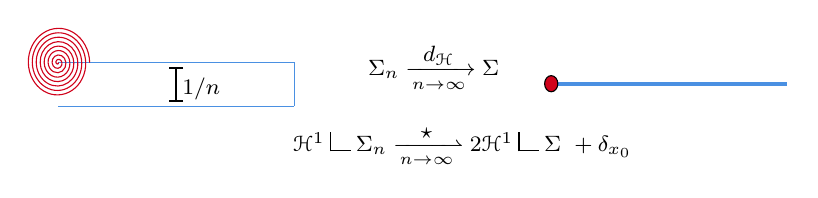
\begin{tikzpicture}[x=0.75pt,y=0.75pt,yscale=-.6,xscale=0.6]
\draw [color={rgb, 255:red, 74; green, 144; blue, 226 } ,draw opacity=1 ] (60.41,81.47) -- (249.96,81.47) ;
\draw [color={rgb, 255:red, 74; green, 144; blue, 226 } ,draw opacity=1 ] (60.41,46.5) -- (249.96,46.5) -- (249.96,81.47) ;
\draw [color={rgb, 255:red, 208; green, 2; blue, 27 } ,draw opacity=1 ] (60.41,46.5) .. controls (60.51,46.5) and (60.59,46.55) .. (60.64,46.65) .. controls (60.7,46.75) and (60.72,46.87) .. (60.68,47.01) .. controls (60.64,47.16) and (60.55,47.3) .. (60.41,47.39) .. controls (60.26,47.5) and (60.08,47.54) .. (59.88,47.53) .. controls (59.66,47.51) and (59.46,47.41) .. (59.27,47.24) .. controls (59.06,47.05) and (58.91,46.8) .. (58.83,46.5) .. controls (58.73,46.16) and (58.73,45.82) .. (58.81,45.46) .. controls (58.9,45.06) and (59.08,44.73) .. (59.36,44.44) .. controls (59.65,44.13) and (60,43.92) .. (60.41,43.83) .. controls (60.86,43.72) and (61.3,43.75) .. (61.74,43.93) .. controls (62.21,44.11) and (62.61,44.43) .. (62.94,44.87) .. controls (63.28,45.33) and (63.5,45.87) .. (63.59,46.5) .. controls (63.68,47.15) and (63.62,47.79) .. (63.39,48.43) .. controls (63.16,49.09) and (62.78,49.65) .. (62.27,50.1) .. controls (61.73,50.57) and (61.11,50.85) .. (60.41,50.95) .. controls (59.69,51.05) and (58.98,50.94) .. (58.3,50.61) .. controls (57.58,50.27) and (56.99,49.74) .. (56.52,49.02) .. controls (56.03,48.27) and (55.74,47.43) .. (55.65,46.5) .. controls (55.56,45.52) and (55.69,44.58) .. (56.06,43.68) .. controls (56.44,42.74) and (57.01,41.96) .. (57.77,41.36) .. controls (58.55,40.73) and (59.44,40.37) .. (60.41,40.26) .. controls (61.42,40.16) and (62.39,40.36) .. (63.33,40.84) .. controls (64.29,41.34) and (65.07,42.09) .. (65.69,43.08) .. controls (66.32,44.1) and (66.68,45.24) .. (66.77,46.5) .. controls (66.86,47.79) and (66.65,49.02) .. (66.15,50.21) .. controls (65.63,51.42) and (64.86,52.41) .. (63.86,53.18) .. controls (62.82,53.97) and (61.68,54.42) .. (60.41,54.51) .. controls (59.12,54.62) and (57.89,54.34) .. (56.71,53.7) .. controls (55.5,53.04) and (54.52,52.07) .. (53.77,50.8) .. controls (52.99,49.51) and (52.56,48.07) .. (52.47,46.5) .. controls (52.38,44.89) and (52.66,43.36) .. (53.31,41.9) .. controls (53.97,40.41) and (54.93,39.2) .. (56.18,38.27) .. controls (57.46,37.33) and (58.87,36.8) .. (60.41,36.7) .. controls (61.99,36.6) and (63.49,36.95) .. (64.91,37.76) .. controls (66.37,38.58) and (67.54,39.76) .. (68.44,41.3) .. controls (69.35,42.88) and (69.86,44.61) .. (69.94,46.5) .. controls (70.04,48.43) and (69.69,50.26) .. (68.9,51.99) .. controls (68.09,53.76) and (66.94,55.18) .. (65.44,56.27) .. controls (63.92,57.38) and (62.24,57.97) .. (60.41,58.08) .. controls (58.55,58.17) and (56.79,57.75) .. (55.12,56.78) .. controls (53.42,55.8) and (52.05,54.41) .. (51.01,52.58) .. controls (49.96,50.74) and (49.39,48.71) .. (49.3,46.5) .. controls (49.2,44.26) and (49.62,42.13) .. (50.56,40.12) .. controls (51.5,38.08) and (52.85,36.43) .. (54.59,35.19) .. controls (56.36,33.92) and (58.3,33.23) .. (60.41,33.14) .. controls (62.56,33.03) and (64.59,33.55) .. (66.5,34.67) .. controls (68.45,35.81) and (70.01,37.43) .. (71.19,39.52) .. controls (72.39,41.64) and (73.03,43.97) .. (73.12,46.5) .. controls (73.21,49.06) and (72.72,51.49) .. (71.65,53.77) .. controls (70.56,56.09) and (69.02,57.95) .. (67.03,59.35) .. controls (65.02,60.77) and (62.81,61.54) .. (60.41,61.64) .. controls (57.99,61.74) and (55.69,61.14) .. (53.53,59.87) .. controls (51.34,58.57) and (49.59,56.74) .. (48.26,54.36) .. controls (46.92,51.96) and (46.21,49.35) .. (46.12,46.5) .. controls (46.03,43.62) and (46.59,40.89) .. (47.8,38.33) .. controls (49.03,35.75) and (50.77,33.66) .. (53,32.1) .. controls (55.26,30.52) and (57.73,29.68) .. (60.41,29.58) .. controls (63.13,29.48) and (65.68,30.14) .. (68.09,31.59) .. controls (70.53,33.04) and (72.48,35.1) .. (73.94,37.74) .. controls (75.42,40.41) and (76.21,43.34) .. (76.3,46.5) .. controls (76.39,49.7) and (75.76,52.71) .. (74.4,55.55) .. controls (73.03,58.42) and (71.1,60.72) .. (68.62,62.44) .. controls (66.11,64.17) and (63.38,65.1) .. (60.41,65.2) .. controls (57.42,65.31) and (54.6,64.55) .. (51.94,62.95) .. controls (49.26,61.34) and (47.12,59.07) .. (45.51,56.15) .. controls (43.89,53.19) and (43.03,49.98) .. (42.94,46.5) .. controls (42.85,42.98) and (43.56,39.66) .. (45.05,36.55) .. controls (46.57,33.41) and (48.69,30.9) .. (51.41,29.02) .. controls (54.17,27.11) and (57.17,26.11) .. (60.41,26.02) .. controls (63.69,25.91) and (66.78,26.74) .. (69.68,28.5) .. controls (72.61,30.27) and (74.94,32.76) .. (76.69,35.96) .. controls (78.46,39.19) and (79.38,42.7) .. (79.47,46.5) .. controls (79.57,50.34) and (78.79,53.95) .. (77.15,57.33) .. controls (75.49,60.75) and (73.18,63.48) .. (70.21,65.52) .. controls (67.21,67.58) and (63.95,68.66) .. (60.41,68.76) .. controls (56.85,68.86) and (53.5,67.95) .. (50.35,66.04) .. controls (47.18,64.11) and (44.65,61.39) .. (42.76,57.93) .. controls (40.85,54.43) and (39.86,50.62) .. (39.77,46.5) .. controls (39.67,42.34) and (40.52,38.44) .. (42.3,34.77) .. controls (44.1,31.08) and (46.61,28.13) .. (49.82,25.93) .. controls (53.07,23.71) and (56.6,22.55) .. (60.41,22.45) .. controls (64.26,22.35) and (67.88,23.34) .. (71.27,25.42) .. controls (74.69,27.52) and (77.41,30.43) .. (79.44,34.18) .. controls (81.49,37.96) and (82.56,42.06) .. (82.65,46.5) .. controls (82.74,50.97) and (81.83,55.18) .. (79.9,59.11) .. controls (77.96,63.08) and (75.26,66.25) .. (71.8,68.61) .. controls (68.31,70.98) and (64.51,72.22) .. (60.41,72.32) .. controls (56.28,72.43) and (52.4,71.36) .. (48.77,69.12) .. controls (45.1,66.86) and (42.18,63.72) .. (40.01,59.71) .. controls (37.82,55.66) and (36.68,51.25) .. (36.59,46.5) .. controls (36.5,41.71) and (37.49,37.2) .. (39.55,32.99) .. controls (41.63,28.75) and (44.53,25.36) .. (48.24,22.85) .. controls (51.97,20.31) and (56.03,18.99) .. (60.41,18.89) .. controls (64.83,18.79) and (68.98,19.94) .. (72.86,22.33) .. controls (76.77,24.75) and (79.88,28.1) .. (82.19,32.4) .. controls (84.53,36.72) and (85.74,41.42) .. (85.83,46.5) ;
\draw (155.19,50.38) -- (155.19,77.59) ;
\draw [shift={(155.19,77.59)}, rotate = 270] [color={rgb, 255:red, 0; green, 0; blue, 0 } ][line width=0.75] (0,5.59) -- (0,-5.59) ;
\draw [shift={(155.19,50.38)}, rotate = 270] [color={rgb, 255:red, 0; green, 0; blue, 0 } ][line width=0.75] (0,5.59) -- (0,-5.59) ;
\draw [color={rgb, 255:red, 74; green, 144; blue, 226 } ,draw opacity=1 ][line width=1.5] (456.45,63.34) -- (646,63.34) ;
\draw [fill={rgb, 255:red, 208; green, 2; blue, 27 } ,fill opacity=1 ] (451.16,63.34) .. controls (451.16,59.76) and (453.53,56.86) .. (456.45,56.86) .. controls (459.38,56.86) and (461.75,59.76) .. (461.75,63.34) .. controls (461.75,66.91) and (459.38,69.81) .. (456.45,69.81) .. controls (453.53,69.81) and (451.16,66.91) .. (451.16,63.34) -- cycle ;

\draw (307.25,28.47) node [anchor=north west][inner sep=0.75pt] [font=\footnotesize] {$\Sigma _{n}\xrightarrow[n\rightarrow\infty ]{\ts\distH} \Sigma $};
\draw (247.12,94.89) node [anchor=north west][inner sep=0.75pt] [font=\footnotesize] {$\cH^{1} \mres \Sigma_{n}\xrightharpoonup[n \rightarrow \infty ]{\ts\star } 2\cH^{1} \mres \Sigma \ +\delta _{x_{0}}$};
\draw (158.07,56.44) node [anchor=north west][inner sep=0.75pt] [font=\footnotesize] {$1/n$};
\end{tikzpicture}
}
\caption{Concentration effects for the weak convergence of measures. Here $\Sigma_n$ is made of two lines getting closer and a spiral converging to a point. In the Hausdorff limit we obtain a segment with shorter length, and a singular limiting measure.}\label{figure.concentration_sets_measure}
\vspace*{-.1\baselineskip}
\end{figure}

Hence, minimizing sequences converge in general to a measure which is
not of the form $\nu_\Sigma$, and we need to determine a relaxation of our energy in a topology for which the Wasserstein distance is lower semi-continuous, such as the narrow convergence.
The relaxed energy takes the form
\begin{equation}\label{problem.shape_optimization_relaxed}
\tag{$\overline{P}_\Lambda$}
\inf_{
\substack{
\nu \in \mathcal{P}_p(\RR^d)
}
}
W_p^p(\rho_0, \nu) + \Lambda \mathcal{L}(\nu),
\end{equation}
where the length functional $\mathcal{L}$, defined in Section~\ref{subsec.deflength}, generalizes the notion of length of the support of a measure, see for instance Example~\ref{example.densities_rectifiable_set}. We~will show later on, in Proposition~\ref{proposition.length_functional_is_lsc},
that $\mathcal{L}$ is the lower semi-continuous relaxation, for the narrow topology, of the functional $\ell$ given by $\cH^1(\Sigma)$ for measures
of the form $\nu_\Sigma$, and $+\infty$ else, see~\eqref{eq:defl}. We~also find that $\mathcal{L}(\nu) < \infty$ if and only if $\supp \nu \in \mathcal{A}$ or $\nu$ is a Dirac mass. The following theorem gathers the various results proved throughout this paper.

\begin{theorem}\label{theorem.the_big_one}
Let $\rho_0 \in \mathcal{P}_p(\RR^d)$, $\Lambda>0$. Then~\eqref{problem.shape_optimization_relaxed} admits a solution $\nu$, and there exists $\Lambda_\star \ge 0$ such that if $\Lambda>\Lambda_\star$, $\nu$ is a Dirac mass. For $\Lambda<\Lambda_\star$, $\nu$ is supported by a set $\Sigma \in \mathcal{A}$ and the following properties hold.
\begin{enumerate}
\item\label{theorem.the_big_one1}
If $\rho_0$ is absolutely continuous with respect to $\cH^1$, or has a $L^\infty$ density with respect to $\cH^1$, then so does $\nu$.
\item\label{theorem.the_big_one2}
If $\rho_0$ does not give mass to $1D$-rectifiable sets, then $\nu=\nu_\Sigma$ and therefore is a solution to the original problem \eqref{problem.shape_optimization}.
\item\label{theorem.the_big_one3}
If $\rho_0 \in L^{\spfrac{d}{d-1}}(\RR^d)$, then $\Sigma$ is Ahlfors regular, \ie there is $r_0$ depending on $d,p,\rho_0$ and $\mathcal{L}(\nu)$ and $C$ depending only on $d,p$ such that for any $x \in \Sigma$ and $r \le r_0$ it holds that
\[
r \le \cH^1(\Sigma \cap B_r(x))\le Cr.
\]
\end{enumerate}
\end{theorem}

The paper is organized as follows: in Section~\ref{section.preliminary_properties} we recall a few tools from optimal transport and geometric measure theory. Next, in Section \ref{section.the_problem} we go through the definition of the length functional and its properties as well as the relaxed problem and the existence of a solution. In Section \ref{section.geometric_properties_transport_map} we discuss
the existence of $\Lambda_\star$.
In Section~\ref{section.solutions_are_absolutely_continuous}
(Theorem~\ref{theorem.solutions_are_absolutely_continuous}) we prove point~\eqref{theorem.the_big_one1} from Theorem \ref{theorem.the_big_one}, while the existence is proved in Section~\ref{section.blowup} (Theorem~\ref{theorem.inR2_density_is_1}),
and the Ahlfors regularity is studied in Section~\ref{section.ahlfors_regularity}.

\section{Preliminaries}\label{section.preliminary_properties}
We start by introducing notions of convergence for sets and measures which will be useful to study problem \eqref{problem.shape_optimization} as well as the relaxed one \eqref{problem.shape_optimization_relaxed}. Next we describe some instrumental properties of the objects we shall use throughout the paper, namely the rectifiable sets and measures.

\Subsection{Convergence of sets and measures}

\subsubsection{Hausdorff and Kuratowski convergence}\label{subsection.Hausdorff_Kuratoski}
We recall some useful definitions of convergence for sets, see for instance~\cite[Chap.\,4]{rockafellar2009variational}, \cite[Chap.\,6]{ambrosio2000functions}.

The Hausdorff distance between two sets $A$, $B$ is defined
as:
\begin{equation}
\label{hausdorff.distance}
\distH(A,B) \eqdef \max\bigl\{\ts
\sup_{a \in A} \dist(a, B),\, \sup_{b \in B} \dist(b, A)
\bigr\},
\end{equation}
where $\dist(\cdot, A)$ denotes the distance function to the set $A$.
A sequence $\left(A_n\right)_{n \in \mathbb{N}}$ of closed subsets of $\RR^d$ converges in the Hausdorff sense to $A$ if $\lim_{n\to\infty} \distH(A_n, A)=0$, and we write $A_n \xrightarrow[n \to \infty]{\distH} A$.
One can prove that this notion of convergence is equivalent to uniform convergence of the distance functions. Since the latter are $1$-Lipschitz, as~a consequence of Arzelà-Ascoli's theorem it follows that if the sequence is contained in a compact set, one can always extract a convergent subsequence. This compactness result is known as \emph{Blaschke's theorem}, see~\cite[Th.\,6.1]{ambrosio2000functions}.

A sequence of closed sets $C_n$ converges in the sense of Kuratowski to $C$, and we write $C_n \xrightarrow[n \to \infty]{K} C$, whenever the two properties hold:
\begin{enumerate}
\item Given a sequence $x_n \in C_n$, all its cluster points are contained in $C$.
\item For all points $x\in C$ there exists a sequence $x_n \in C_n$, converging to $x$.
\end{enumerate}
Again, one can show that $C_n\to C$ in the sense of Kuratowski
if and only if $\dist(x,C_n)\to\dist(x,C)$ (possibly infinite if $C=\emptyset$) locally uniformly (see~\cite[Cor.\,4.7]{rockafellar2009variational}). In addition, the Bolzano-Weierstrass property holds for the Kuratowski convergence as well, \ie any sequence of closed sets has a subsequence which converges, possibly to the empty set.

It is classical that Hausdorff and Kuratowski convergences coincide on sequences on uniformly bounded compact sets, the next lemma describes a more subtle relationship. We~prove it in Appendix~\ref{appendix.kuratowski_convergence}.
\begin{lemma}\label{lemma.localized_Kuratowski}
Let $(C_n)_{n \in \mathbb{N}}$ be a sequence of closed sets in $\RR^d$, converging to $C$ in the sense of Kuratowski.
Then, for any $x \in \RR^d$,
\[
C_n\cap\overline{B_R(x)}
\xrightarrow[n \to \infty]{\distH}
C\cap\overline{B_R(x)},
\]
for every radius $R>0$ such that $\overline{C\cap B_R(x)} = C\cap \overline{B}_R(x)$. Moreover, that condition holds for all $R>0$ except in a countable set.
\end{lemma}

\subsubsection{Convergence of measures}
Given a Borel set $X\subset \RR^d$, we~denote by $\mathcal{M}(X)$ (\resp $\mathcal{M}_+(X)$) the collection of the finite (\resp finite positive) Radon measures on~$X$.
The space of Borel probability measures on $X$ is denoted by $\mathcal{P}(X)$, and $\mathcal{P}_p(X)$ refers to its subset of probability measures with finite $p$-moment ($p\ge 1$).

Following~\cite{ambrosio2000functions}, we~say that a sequence $\left(\mu_n\right)_{n \in \mathbb{N}}$ of Radon measures on $\RR^d$ locally weakly-$\star$ converges to some Radon measure $\mu$, if, for every continuous function with compact support $\phi \in C_c(\RR^d)$,
\begin{equation}\label{eqRadonweakstar}
\int_{\RR^d} \phi \dd \mu_n
\xrightarrow[n \to \infty]{}
\int_{\RR^d} \phi \dd \mu.
\end{equation}
Any sequence $(\mu_n)_{n\in\mathbb{N}}$ of Radon measures such that $\sup_{n\in\mathbb{N}} \abs{\mu_n}(K)<+\infty$ for every compact set $K\subset \RR^d$ has a locally weakly-$\star$ convergent subsequence.

If $\left\{\mu_n\right\}_{n \in \mathbb{N}}\subset \mathcal{M}(\RR^d)$ is a sequence of \emph{finite} Radon measures and~\eqref{eqRadonweakstar} holds for every bounded continuous function $\phi\in C_b(\RR^d)$, we~say that $\mu_n$ narrowly converges to $\mu$, and we write $\mu_n \xrightharpoonup[n \to \infty]{} \mu$. When $(\mu_n)_{n\in\mathbb{N}}$ is a sequence of probability measures, that convergence is often referred to as the \emph{weak convergence} of probability measures.

If $X$ is compact, any sequence of probability measures $\{\mu_n\}_{n\in\mathbb{N}}\subset \mathcal{P}(X)$ has a weakly convergent subsequence.
More generally, if $X$ is not compact, compactness for the narrow convergence requires the assumptions of Prokhorov's theorem,
see~\hbox{\cite[Th.\,2.8]{ambrosio2021lectures}}.

\subsubsection{Optimal transport and the Wasserstein distance}
\label{sec:wasserstein}

The Wasserstein distan\-ces~$W_p$ are defined through the value function of an optimal transport problem, see~\cite{ambrosio2008gradient,santambrogio2015optimal,villani2009optimal} for details. Given two probability measures $\mu, \nu \in \mathcal{P}_p(\RR^d)$, we~set
\begin{equation}\label{wasserstein_distance}
W_p^p(\mu, \nu)
\eqdef
\min_{\gamma \in \Pi(\mu, \nu)}
\int_{\RR^d\times \RR^d} |x - y|^p\dd\gamma,
\end{equation}
where
$\Pi(\mu, \nu) \eqdef
\left\{
\gamma \in \mathcal{P}\left(\RR^d\times \RR^d\right) :
\,
{\pi_{0}}_\sharp\gamma = \mu, \
{\pi_{1}}_\sharp\gamma = \nu
\right\}
$
is the space of transport couplings, and $\pi_i$ denote the projections, \ie $\pi_0(x,y) = x$ and $\pi_1(x,y) = y$. Whenever~$\mu$ does not have atoms, the value of \eqref{wasserstein_distance} coincides with
\begin{equation}\label{wasserstein_distance.monge}
\inf_{
\substack{
T_{\sharp}\mu = \nu
}
}
\int_{\RR^d} |x - T(x)|^p\dd \mu,
\end{equation}
where the inf is taken over all measurable maps $T$ such that $T_\sharp\mu(A) = \nu(A) = \mu(T^{-1}(A))$ for any Borel set $A$.

The optimal transport problem can be analogously defined for any pair of positive $\mu, \nu$ in $\mathcal{M}_+(\RR^d)$. In this case, the Wasserstein distance becomes a 1-homogeneous functional and is finite if and only if the measures have finite $p$-moments and the same total mass $\mu(\RR^d) = \nu(\RR^d)$.

The Wasserstein distance is l.s.c.~with respect to the narrow convergence, and continuous in a compact domain, \cite[Lem.\,4.3]{villani2009optimal}.

\newcommand{\Golab}{Go\l\k{a}b}
\subsection{\Golab's theorem}
We now study the lower semicontinuity of~\eqref{problem.shape_optimization}.
``\Golab's theorem''~\cite{Golab} shows that along sequences of connected sets, the length is lower semi-continuous with respect to the Hausdorff convergence~\cite[Chap.\,10]{morel2012variational}.
It is of course also true if the sequence has a uniformly bounded number of connected components.

The issue is that the compactness of Hausdorff convergence is not transferred to the weak convergence of measures of the form $\cH^1\mres \Sigma$ which may concentrate in the limit.
In general, one can prove the following:
\begin{theorem}[Density version of \Golab's theorem]\label{theorem.Golab_localversion}
Let ${(\Sigma_n)}_{n \in \mathbb{N}}$ be a sequence of closed and connected subsets of $\RR^d$ converging in the sense of Kuratowski to some closed set $\Sigma$ and having locally uniformly finite length, \ie for all $R > 0$
\[
\sup_{n \in \mathbb{N}} \cH^1(\Sigma_n \cap B_R(x_0)) < +\infty.
\]
Define the measures $\mu_n \eqdef \cH^1\mres \Sigma_n$, and let $\mu$ be a local weak-$\star$ cluster point of this sequence. Then $\supp\mu \subset \Sigma$ and it holds that
\[
\mu \ge \cH^1\mres \Sigma,
\]
in the sense of measures.
\end{theorem}
Such a result is hidden in the proof in~\cite{ambrosio2004topics} of the usual thesis of \Golab's theorem, see also~\cite{paolini2013existence}. Yet in this variant, we~consider a Kuratowski convergence and do not restrict the sets to be uniformly bounded, or have bounded lengths.
This is useful for the proof of Theorem~\ref{theorem.Gamma_convergence} where we consider sequences of blow-ups of sets. The proof of Theorem~\ref{theorem.Golab_localversion} is given in Appendix~\ref{appendix.kuratowski_convergence}.

\subsection{Rectifiable sets and measures}
We now introduce
the notions of \emph{rectifiable sets} and \emph{rectifiable measure}, which will be crucial for understanding the fine
properties of the elements of $\mathcal{A}$.
\begin{definition}
Let $M \subset \RR^d$ be a Borel set and $k \in \mathbb{N}$, we~say that $M$ is countably $\cH^k$-rectifiable, or shortly $k$ rectifiable, if there are countably many Lipschitz functions $f_i: \RR^k \to \RR^d$ such that
\[
\cH^k\Bigl(
M \setminus \bigcup_{i \in \mathbb{N}} f_i(\RR^k)
\Bigr)
= 0.
\]
A Radon measure $\mu$ is said to be $k$-rectifiable if it is supported over a $k$-rectifiable set and $\mu \ll \cH^k$.
\end{definition}

In the simple case $M = f(E)$, for $E \subset \RR^k$, one can define the tangent space at a point of differentiability of $f$ as
\[
\nabla f(z)(\RR^k), \quad\text{for $x = f(z)$}.
\]
This is a parametric definition that can be extended to $k$-rectifiable sets. It turns out the parametric notion of tangentiability can be expressed in terms of measure theory. Given a Borel set $M$, we~set the measure $\mu = \cH^k\mres M$, and we consider the family of blow-up measures
\begin{equation}\label{blowup_measure_operator}
\mu_r \eqdef r^{-k} \Phi^{x,r}_\sharp \mu = \cH^k\mres \Bigl(\frac{M - x}{r}\Bigr), \quad\text{for }
\Phi^{x,r}\eqdef \frac{\text{id} - x}{r}.
\end{equation}

If $M$ is countably $\cH^k$-rectifiable, and $\cH^k(M\cap K)<+\infty$ for every compact set~$K$, we~say that $M$ is locally $\cH^k$-rectifiable, and then the blow-up theorem, see~\cite[Th.\,10.2]{maggi2012sets}, states that for $\cH^k$-a.e.\ $x \in M$ this family of measures converges in the weak-$\star$ topology to a measure of the form $\cH^k \mres \pi_x$, for a unique $k$-plane $\pi_x \in \text{G}(k,d)$, the Grassmannian of $k$-planes of $\RR^d$.

More generally define the $k$-density, whenever the limit exists, of a Radon measure~$\mu$ as
\begin{equation}\label{eq.k_density}
\theta_k(\mu,x) \eqdef \lim_{r \to 0^+}
\frac{\mu(B_r(x))}{\omega_k r^k}\quad \text{ and }\quad
\theta_k(M,x) \eqdef \theta_k(\cH^k\mres M, x),
\end{equation}
where $\omega_k$ is the volume of the unit $k$-dimensional ball, see~\cite{ambrosio2000functions,maggi2012sets}. A direct consequence of the blow-up theorem is that $\cH^k$-a.e.~point of a $k$-rectifiable set has $k$-density $1$. Analogously for a $k$-rectifiable measure $\mu$ it holds that $\mu = \theta_k(\mu, x) \cH^k\mres M$.

The equivalence between all notions was completed with the work of Preiss and the notion of a tangent space to a measure, see for instance the monograph~\cite{delellis2006lecture}. It~implies that a measure (\resp a set) which has almost everywhere a finite and non zero $k$-density is $k$-rectifiable. In particular, one has the following theorem.

\begin{theorem}\label{theorem.rectifiability_tangentiability}
Let $\mu$ be a Radon measure over $\RR^d$, the following are equivalent.
\begin{enumeratei}
\item\label{theorem.rectifiability_tangentiabilityi}
$\mu$ is $k$-rectifiable.
\item\label{theorem.rectifiability_tangentiabilityii}
For $\cH^k$-a.e. $x \in \supp \mu$, the limit in~\eqref{eq.k_density} exists and
\[
r^{-k}\Phi^{x,r}_\sharp \mu \xrightharpoonup[r \to 0]{\ts\star} 
\theta_k(\mu,x)\cH^k\mres \pi_x,
\]
for a unique $k$-plane $\pi_x \in \text{G}(k,d)$.
\item\label{theorem.rectifiability_tangentiabilityiii}
For $\cH^k$-a.e. $x \in \supp \mu$, the $k$-density of $\mu$ in \eqref{eq.k_density} exists, is finite and positive.
\end{enumeratei}
\end{theorem}

In the previous theorem, if we take $\mu = \cH^k\mres M$ where $M$ is a countably $\cH^k$\nobreakdash-rectifiable set we define the \emph{approximate tangent space} of $M$ at $x$ as $T_x M \eqdef \pi_x$, where $\pi_x$ is the unique $k$-plane from point \eqref{theorem.rectifiability_tangentiabilityii}.

\begin{definition}\label{definiton.rectifiability_point}
Let $M\subset \RR^d$ be a $k$-rectifiable set. We~say that $x \in M$ is a rectifiability point when the locally weakly-$\star$ convergence of point \eqref{theorem.rectifiability_tangentiabilityii} from Theorem~\ref{theorem.rectifiability_tangentiability} holds, with $\mu = \cH^k\mres M$ and $\theta_k(\mu,x)=1$.
\end{definition}

Now we pass to our case of interest, of compact connected sets $\Sigma$ with finite length, $\mathcal{H}^1(\Sigma) < +\infty$, in view of~\eqref{admissible_set}. From~\cite[Prop.\,30.1 \& Cor.\,30.2]{david2006singular} or~\cite[Th.\,4.4]{alberti2017structure}, any compact connected set with finite length is also path-connected, \ie any pair of its points can be joined by a continuous arc. Such sets are also known to be $1$-rectifiable, see~\cite[Th.\,4.4.8]{ambrosio2004topics}, and hence they enjoy the properties of Theorem \ref{theorem.rectifiability_tangentiability}. In the next lemma, we~show that the blow-up of some $\Sigma \in \mathcal{A}$ around a rectifiability point is precisely its approximate tangent space.

\begin{lemma}\label{lemma.blowup_domain_measure}
Given $\Sigma \in \mathcal{A}$, then for $\cH^1$-a.e.\ $y \in \Sigma$, it holds that
\[
\frac{\Sigma - y}{r} \xrightarrow[r \to 0^+]{\ts K} T_y\Sigma
\quad \text{and} \quad
\frac{\Sigma - y}{r}\cap \overline{B_R(0)} \xrightarrow[r \to 0^+]{\ts\distH} T_y\Sigma\cap \overline{B_R(0)}, \text{ for all $R>0$.}
\]
\end{lemma}

\begin{proof}
First we take a rectifiability point $y \in \Sigma$ with tangent space $T_y\Sigma$,
by Theorem~\ref{theorem.rectifiability_tangentiability} such points cover $\cH^1$-a.a.~of $\Sigma$.
In particular, point \eqref{theorem.rectifiability_tangentiabilityii} of the theorem shows that
\[
\cH^1\mres((\Sigma-y)/r)\xrightharpoonup[r \to 0]{\star} \cH^1\mres T_y\Sigma.
\]
Let $T$ be the (Kuratowski) limit of a subsequence $(\Sigma-y)/r_k$.
Clearly, the limit measure $\cH^1\mres T_y\Sigma$ is supported by $T$, hence $T_y\Sigma\subset T$.
Thanks
to Lemma~\ref{lemma.localized_Kuratowski} and Theorem~\ref{theorem.Golab_localversion}, for
almost all $R>0$,
\begin{equation}
\cH^1(T\cap B_R) \le \liminf_{k\to\infty} \cH^1\Bigl(\frac{\Sigma-y}{r_k}\cap B_R\Bigr)
= \cH^1(T_y\Sigma\cap B_R),\label{eq.blowup_domain_measure}
\end{equation}
which shows that up to a $\cH^1$-negligible set, $T=T_y\Sigma$.

Notice that, if there is some $x \in T\setminus T_y\Sigma$, we~may consider some ball $B_s(x)$ which does not intersect $T_y\Sigma$. Since $T$ is the limit of connected sets, $x$ must be path-connected in $T$ to some point in $(B_s(x))^c$, so~that $\cH^1(T\cap B_s(x))\ge s$. This contradicts~\eqref{eq.blowup_domain_measure}. Hence $T=T_y\Sigma$, and is independent of the subsequence, and we deduce that $(\Sigma-y)/r\stackrel{K}{\to} T_y\Sigma$. The convergence in the Hausdorff distance follows from Lemma~\ref{lemma.localized_Kuratowski}.
\end{proof}

\section{The length functional and the relaxed problem}\label{section.the_problem}
If a minimizing sequence $\Sigma_n$ converges to some set $\Sigma$, we~cannot expect weak cluster points of the measures $\nu_{\Sigma_n}$ to have the form $\nu_\Sigma$, see Figure~\ref{figure.concentration_sets_measure}. Hence the objective of \eqref{problem.shape_optimization} is not lower semi-continuous for the narrow convergence, and, in this section, we~introduce a relaxation for \eqref{problem.shape_optimization}. First, we~define a functional which extends the length of the support and we discuss some of its properties, then we use it to define the relaxed problem.

\subsection{Definition and elementary properties}\label{subsec.deflength}
Recalling that $\mathcal{A}$ is the collection of the compact connected sets $\Sigma \subset \RR^d$ with $0<\cH^1(\Sigma)<+\infty$, we~consider
\begin{equation}\label{eq:defl}
\ell : \mathcal{P}(\RR^d) \ni \nu \mto
\begin{cases}
\cH^1(\Sigma) & \text{if $\nu=\dfrac{1}{\cH^1(\Sigma)}\,\cH^1\mres \Sigma$ for some $\Sigma \in \mathcal{A}$},\\
+\infty& \text{otherwise,}
\end{cases}
\end{equation}
so that \eqref{problem.shape_optimization} becomes $\inf_\nu W_p^p(\rho_0, \nu) + \Lambda\ell(\nu)$. As discussed above, $\ell$ is not l.s.c., hence we introduce the following relaxation, which we call the \emph{length functional}. For any $\nu \in \mathcal{P}(\RR^d)$, we~define
\begin{equation}
\mathcal{L}(\nu)
\eqdef
\begin{cases}
\inf \enscond{\alpha \ge 0}{\alpha \nu \ge \cH^1\mres \supp \nu} & \mbox{if $\supp \nu$ is connected,}\\
+\infty & \mbox{otherwise,}
\end{cases}\label{lengthalpha}
\end{equation}
with the convention that $\inf \emptyset \eqdef +\infty$. Notice that, since $\nu$ is a probability measure, $\mathcal{L}(\nu)\geq \cH^1(\supp \nu)$, and that $\mathcal{L}(\nu)=0$ if and only if $\nu = \delta_x$ for some $x \in \RR^d$. As~a~result, $0<\mathcal{L}(\nu) < \infty$ if and only if $\supp \nu \in \mathcal{A}$. Moreover, for any $\Sigma \in \mathcal{A}$ and $ \nu_\Sigma\eqdef\Psfrac{1}{\cH^1(\Sigma)} \cH^1\mres \Sigma$, we~have $\mathcal{L}(\nu_\Sigma) = \cH^1(\Sigma)=\ell(\nu_\Sigma)$.

\begin{remark}
Definition~\eqref{lengthalpha} also makes sense for any positive measure $\mu \in \mathcal{M}_+(\RR^d)$. In that case, thanks to Theorem~\ref{theorem.Golab_localversion}, it may be easily shown to be
lower semi-continuous with respect to the weak convergence,
defining $\mathcal{L}(0)=0$ (see also Section~\ref{sec.length_functional_is_lsc}).
Yet then, of course, even for uniformly distributed measures such as $\nu = \theta\cH^1\mres \Sigma$ for some $\theta> 0$, its value does not coincide with the length of the support anymore (it rather is $\cH^1(\Sigma)/\nu(\RR^d)$).
\end{remark}

In Section~\ref{sec.length_functional_is_lsc} below, we~prove that $\mathcal{L}$ is the lower semi-continuous envelope of~$\ell$ for the narrow topology of probability measures. Before that, let us discuss some alternative formulations for $\mathcal{L}$. Following~\cite[\S 2.4]{ambrosio2000functions}, we~consider the upper derivative,
\begin{equation}
\forall x \in \supp\nu,\quad D^+_\nu(\cH^1\mres \supp\nu)(x) \eqdef \limsup_{r\to 0^+} \frac{\cH^1(B_r(x)\cap \supp \nu)}{\nu(B_r(x))}.
\end{equation}

\begin{proposition}[Alternative definitions of $\mathcal{L}$]
Let $\nu \in \mathcal{P}(\RR^d)$ be such that $\supp \nu$ is connected. Then
\begin{align}
\mathcal{L}(\nu) &=\sup \Benscond{\frac{\cH^1(U \cap \supp \nu)}{\nu(U)}}{U \,\text{open},\, U\cap \supp \nu\neq \emptyset}\label{lengthopen}\\
&=\sup \Benscond{\frac{\cH^1(B_r(x)\cap \supp \nu)}{\nu(B_r(x))}}{r>0,\, x \in \supp \nu} \label{lengthball}\\
&= \norm{D^+_\nu(\cH^1\mres \supp\nu)}_{\infty},\label{lengthderiv}
\end{align}
where $\norm{\cdot}_\infty$ denotes the supremum norm over $\supp \nu$.
\end{proposition}

\begin{proof}
It is immediate that
\begin{equation*}
\left(\mbox{R.H.S. of \eqref{lengthalpha}}\right)\geq \left(\mbox{R.H.S. of \eqref{lengthopen}}\right)\geq \left(\mbox{R.H.S. of \eqref{lengthball}}\right)\geq(\mbox{R.H.S. of \eqref{lengthderiv}}).
\end{equation*}
Now, assume that $\norm{D^+_\nu(\cH^1\mres \supp\nu)}_{\infty}<+\infty$ and let $\alpha > \norm{D^+_\nu(\cH^1\mres \supp\nu)}_{\infty}$. For every compact set $K \subset \RR^d$ and every $x \in K\cap \left(\supp \nu\right)$, there is some $r(x)>0$ such that $\cH^1\left(B_r(x)\cap \left(\supp \nu\right)\right)\leq \alpha \nu(B_r(x))$. We~may extract from the covering $(B_{r(x)}(x))_{x \in K\cap \left(\supp\nu\right)}$ with open sets a finite covering $(B_{r_i}(x_i))_{i=1}^{N}$ of $K\cap \left(\supp \nu\right)$. As a result
\begin{equation*}
\cH^1(K\cap \left(\supp\nu\right))\leq \sum_{i=1}^{N} \alpha \nu(B_{r_i}(x_i))\leq N\alpha<+\infty,
\end{equation*}
so that $\cH^1\mres\left(\supp\nu\right)$ is a Radon measure. We~may thus apply~\cite[Prop.\,2.21]{ambrosio2000functions} to deduce
\begin{equation*}
\left(\mbox{R.H.S. of \eqref{lengthderiv}}\right)\geq(\mbox{R.H.S. of \eqref{lengthalpha}}).
\end{equation*}
If $\norm{D^+_\nu(\cH^1\mres \supp\nu)}_{\infty}=+\infty$, the inequality holds trivially, which completes the proof.
\end{proof}

The length functional inherits some of the properties of the $\cH^1$ measure.
\begin{proposition}\label{prop.length.lipschitz}
Let $f\colon \RR^d\rightarrow \RR^d$, be a $k$-Lipschitz function, with $k>0$. Then
\begin{equation}
\forall \nu \in \mathcal{P}(\RR^d),\quad \cL(f_\sharp\nu)\leq k \cL(\nu). \label{eq.lipschitzlength}
\end{equation}
\end{proposition}

\begin{proof}
If $\cL(\nu)=+\infty$, there is nothing to prove. Otherwise, $\supp \nu$ is compact, and $\supp(f_\sharp \nu)= f(\supp \nu)$.
Moreover, for any open set $U \subset \RR^d$, since $f^{-1}(U)$ is open,
\begin{equation*}
U\cap \left(\supp f_\sharp \nu\right)\neq \emptyset \iff \nu(f^{-1}(U))>0 \iff f^{-1}(U)\cap \left(\supp \nu\right)\neq \emptyset.
\end{equation*}

Now, let $U$ be an open set which intersects $\supp(f_\sharp \nu)$. Using that
\begin{equation*}
U\cap f(\supp \nu) \subset f\bigl(f^{-1}(U)\cap \supp \nu\bigr),
\end{equation*}
we get
\begin{align*}
\frac{\cH^1\left(U\cap \supp (f_\sharp \nu)\right)}{f_\sharp\nu(U)}= \frac{\cH^1\left(U\cap f(\supp \nu))\right)}{\nu(f^{-1}(U))}
&\leq \frac{\cH^1\left(f\left(f^{-1}(U)\cap \supp \nu\right)\right)}{\nu(f^{-1}(U))}\\
&\leq k\frac{\cH^1\left(f^{-1}(U)\cap \supp \nu\right)}{\nu(f^{-1}(U))}\\
&\leq k\mathcal{L}(\nu),
\end{align*}
since $f^{-1}(U)$ is an open set which intersects $\supp \nu$.
Taking the supremum over all $U$ yields the claimed inequality.
\end{proof}

It is also possible to express the length-functional using the Besicovitch differentiation theorem~\cite[Th.\,2.22]{ambrosio2000functions}. Assume that $\cH^1(\supp \nu)<+\infty$ (otherwise $\mathcal{L}(\nu)=+\infty$). Then, the measure $\cH^1\mres \supp\nu$ is Radon, and the limit
\begin{align}
D_\nu(\cH^1\mres \supp\nu)(x)&\eqdef \lim_{r \to 0^+} \frac{\cH^1(B_r(x)\cap \supp \nu)}{\nu(B_r(x))} \\ \bigg(\mbox{\resp} D_{\cH^1\mres \supp\nu}(\nu)(x)&\eqdef \lim_{r \to 0^+}\frac{\nu(B_r(x))}{\cH^1(B_r(x)\cap \supp \nu)}\bigg)
\end{align}
exists for $\nu$-a.e.\ $x$ (\resp $\cH^1\mres \supp\nu$-a.e.\ $x$).
\begin{proposition}[Alternative definitions, II]\label{prop.length.besico}
Let $\nu \in \mathcal{P}(\RR^d)$ such that $\supp \nu$ is connected and $\cH^1(\supp \nu)<+\infty$. Then
\begin{align}
\mathcal{L}(\nu) &=
\begin{cases}
\Bnorm{\dfrac{\dd(\cH^1\mres \supp\nu)}{\dd \nu}}_{L^{\infty}_\nu} & \mbox{if $\left(\cH^1\mres \supp \nu\right) \ll \nu$,}\\
+\infty &\mbox{otherwise.}
\end{cases}\label{length_besico1}\\
&=
\begin{cases}
0 & \mbox{if $\supp \nu$ is a singleton,}\\
\Bnorm{\Bigl(\dfrac{\dd \nu}{\dd(\cH^1\mres \supp\nu)}\Bigr)^{-1}}_{L^{\infty}_{\cH^1\mres \supp\nu}} & \mbox{otherwise}.
\end{cases}\label{length_besico2}
\end{align}
\end{proposition}
Notice that in Proposition~\ref{prop.length.besico}, both ``norms'' may take the value $+\infty$, and in \eqref{length_besico2}, we~adopt the convention that $1/0=+\infty$.

\begin{proof}[Proof of Proposition \ref{prop.length.besico}]
First, we~prove \eqref{length_besico1}. If $\left(\cH^1\mres \supp \nu\right) \ll \nu$ then the Lebesgue-Besicovitch differentiation theorem ensures that
\begin{equation*}
\cH^1\mres \supp \nu = \Bigl(\frac{\dd \left(\cH^1\mres \supp\nu\right)}{\dd \nu}\Bigr)\nu \leq \Bnorm{\frac{\dd \left(\cH^1\mres \supp\nu\right)}{\dd \nu}}_{L^{\infty}_\nu}\nu.
\end{equation*}
Therefore,
\begin{equation*}
\mathcal{L}(\nu)\leq \Bnorm{\frac{\dd \left(\cH^1\mres \supp\nu\right)}{\dd \nu}}_{L^{\infty}_\nu} \leq \norm{D^+_\nu(\cH^1\mres \supp\nu)}_{\infty}=\mathcal{L}(\nu).
\end{equation*}
If $\left(\cH^1\mres \supp \nu\right)$ is not absolutely continuous with respect to $\nu$, there is no $\alpha>0$ such that $\alpha \nu \geq \cH^1\mres \supp\nu$, and $\mathcal{L}(\nu)=+\infty$.

Now, we~prove \eqref{length_besico2}. The case where $\supp \nu$ is a singleton is already known. We~\hbox{assume} now that $\cH^1(\supp \nu)>0$, and using the Besicovitch differentiation theorem~\cite[Th.\,2.22]{ambrosio2000functions}, we~decompose
\begin{equation}
\nu = \theta\cH^1\mres \supp \nu + \nu^s,\label{eq-besico-decompo}
\end{equation}
where
\[
\theta(x)\eqdef \frac{\dd \nu}{\dd \left(\cH^1\mres \supp\nu\right)}(x)= \lim_{r \to 0^+} \frac{\nu(B_r(x))}{\cH^1(B_r(x)\cap \supp \nu)} =\left(D^+_\nu(\cH^1\mres \supp\nu)(x)\right)^{-1}
\]
for $\left(\cH^1\mres \supp\nu\right)$-a.e.\ $x$. From the last equality, we~get
\begin{equation*}
\norm{\theta^{-1}}_{L^{\infty}_{\cH^1\mres \supp\nu}} \leq \norm{D^+_\nu(\cH^1\mres \supp\nu)(x)}_\infty =\mathcal{L}(\nu).
\end{equation*}
To prove the converse inequality, we~assume $\norm{\theta^{-1}}_{L^{\infty}_{\cH^1\mres \supp\nu}}<+\infty$ (otherwise there is nothing to prove). Using~\eqref{eq-besico-decompo}, we~note that
\begin{equation*}
\Bigl(\norm{\theta^{-1}}_{L^{\infty}_{\cH^1\mres \supp\nu}}\Bigr)\nu \ge \cH^1\mres \supp\nu,
\end{equation*}
so that $\mathcal{L}(\nu)\le \norm{\theta^{-1}}_{L^{\infty}_{\cH^1\mres \supp\nu}}$.
\end{proof}

We may now examine a few examples.
\begin{example}\label{example.diracs_dense_sequence}
Let $\nu=\sum_{n=1}^{\infty} 2^{-n}\delta_{q_n}$, where $(q_{n})_{n\ge 1}$ is a dense sequence in $\ci{0}{1}$. The support being the set of points $x$ such that $\nu(B_r(x)) > 0$ for all $r>0$, one has $\supp \nu = [0,1]$ which is connected. However, using \eqref{lengthalpha}, we~see that $\mathcal{L}(\nu)=+\infty$.
\end{example}

\begin{example}[Densities on a $(\cH^1,1)$-rectifiable set]\label{example.densities_rectifiable_set}
Let $\Sigma \subseteq \RR^d$ be a closed connected set with $0<\cH^1(\Sigma)<+\infty$, $\theta\colon \Sigma \rightarrow \RR_+$ a Borel function such that $ \int_\Sigma \theta\dd \cH^1 < 1$, and let $\nu = \theta \cH^1\mres \Sigma + \nu^s$ be a probability measure, where $\supp \nu^s \subset \Sigma$ and the measures $\nu^s$ and $\cH^1\mres\Sigma$ are mutually singular.
Then $\mathcal{L}(\nu)= \norm{1/\theta}_{L^\infty_{\cH^1\mres \Sigma}}$: the length functional ignores the singular part.
\end{example}

\begin{example}[Parametrized Lipschitz curves]\label{example.parametrized_curve}
Let $\gamma\colon \ci{0}{1}\rightarrow \RR^d$ be a non-constant Lipschitz curve, and let $\nu$ such that for all $f \in C_b(\RR^d)$,
\[
\langle f, \nu\rangle \eqdef \frac{1}{\len(\gamma)}\biggl(\int_0^1f(\gamma(t))\abs{\dot\gamma(t)}\dd t\biggr),
\]
where $\len(\gamma)\eqdef \int_0^1 \abs{\dot\gamma(t)}\dd t$ is the length of the curve.
By the area formula~\cite[Th.\,3.2.5]{federer2014geometric},
\begin{equation*}
\dd\nu(y)= \frac{1}{\len(\gamma)} \card(\gamma^{(-1)}(y))\dd\left( \cH^1\mres \Sigma\right)(y),
\end{equation*}
where $\Sigma=\gamma(\ci{0}{1})$. As a result,
\begin{equation}
\mathcal{L}(\nu) = \frac{\len(\gamma)}{\mathrm{ess}\mbox{-}\min_{y \in\Sigma}\left(\card(\gamma^{(-1)}(y))\right)},
\end{equation}
where the minimum is an \emph{essential minimum} with respect to $\cH^1\mres \Sigma$.
\end{example}

\subsection{Lower semi-continuity of the length functional}
\label{sec.length_functional_is_lsc}
Now, we~prove that $\mathcal{L}$ is the lower semi-continuous envelope of $\ell$ for the narrow convergence.

\begin{proposition}
\label{proposition.length_functional_is_lsc}
The functional $\mathcal{L}$ is the lower semi-continuous envelope of $\ell$ for the narrow topology. Moreover, for every $\nu$ such that $\mathcal{L}(\nu)<+\infty$,
\begin{equation}\label{lenghtineq}
\cH^1(\supp \nu)\leq \mathcal{L}(\nu),
\end{equation}
with equality if and only if either $\nu=\delta_x$ for some $x \in \RR^d$ (if $\cH^1(\supp\nu)=0$), or~$\cH^1(\supp\nu)>0$ and $ \nu=\Psfrac{1}{\cH^1(\supp \nu)}\cH^1\mres \supp \nu$, \ie $\nu = \nu_\Sigma$ for some $\Sigma \in \mathcal{A}$, as defined in~\eqref{admissible_set}.
\end{proposition}

\begin{proof}[Proof of Proposition \ref{proposition.length_functional_is_lsc}]
The inequality \eqref{lenghtineq} is clear from the definition of \eqref{lengthalpha}, so~we study the equality case.

If $\nu=\delta_x$ or $\nu=\Psfrac{1}{\cH^1(\supp \nu)}\cH^1\mres \supp \nu$ with $\cH^1(\supp\nu)>0$, one readily checks that $\mathcal{L}(\nu)=\cH^1(\supp \nu)$.
Conversely, if \eqref{lenghtineq} is an equality, for every Borel set $B$,
\begin{align*}
0 &= \mathcal{L}(\nu)-\cH^1(\supp\nu) \\
&= \underbrace{\left(\mathcal{L}(\nu)\nu(B)-\cH^1(B\cap \supp\nu)\right)}_{\geq 0}+ \underbrace{\left(\mathcal{L}(\nu)\nu(B^\complement)-\cH^1(B^\complement\cap \supp\nu)\right)}_{\geq 0},
\end{align*}
so that both terms must be zero. If $\mathcal{L}(\nu)>0$, we~deduce
\begin{equation*}
\forall B\subset \RR^d\ \mbox{Borel},\quad \nu(B) = \frac{\cH^1(B\cap \supp\nu)}{\mathcal{L}(\nu)}= \frac{\cH^1(B\cap \supp\nu)}{\cH^1(\supp \nu)}.
\end{equation*}
If $\mathcal{L}(\nu)=0$, $\cH^1(\supp\nu)=0$ and since $\supp \nu$ is connected, $\nu$ is a Dirac mass.

Next we prove that $\mathcal{L}$ is sequentially lower semi-continuous. We~consider $(\nu_{n})_{n\in \mathbb{N}}$ such that $\nu_n \xrightharpoonup[n \to \infty]{} \nu \in \mathcal{P}(\RR^d)$ and we show that $\alpha \eqdef \liminf_{n \to \infty} \mathcal{L}(\nu_n) \geq \mathcal{L}(\nu)$. If~$\alpha\!=\!+\infty$, we~have nothing to prove. Otherwise, up to the extraction of a subsequence, we~may assume that $\lim_{n \to \infty} \mathcal{L}(\nu_n)=\alpha$ and that $\mathcal{L}(\nu_n)<+\infty$ for all $n \in \mathbb{N}$.

Defining the sequence of compact and connected sets $\Sigma_n \eqdef \supp \nu_n$, it holds that $\cH^1(\Sigma_n) \le \mathcal{L}(\nu_n)$, so~that
\[
\sup_{n\geq N} \cH^1(\Sigma_n) \leq \alpha +1 <+\infty
\]
for $N$ large enough. Hence, for all $n\ge N$, $\diam(\Sigma_n)\leq \alpha +1$. In addition, let $x\in \supp \nu$. Since $0<\nu(B_1(x))\leq \liminf_{n\to \infty}\nu_n(B_1(x))$, for all $n$ large enough $\left(\supp \nu_n\right)\cap B_1(x)\neq \emptyset$, thus $\supp \nu_n \subset \overline{B_{\alpha+2}(x)}$.

Therefore, we~may apply Blaschke's theorem and assume,
up to extracting a subsequence, that $\Sigma_n \xrightarrow[n \to \infty]{\distH} \Sigma$. From the weak convergence of measures one has $\supp \nu \subset \Sigma$. Let us show that $\supp \nu = \Sigma$. If $\Sigma$ is a singleton $\{x_0\}$, we~have $\nu = \delta_{x_0}$. Otherwise, Theorem~\ref{theorem.Golab_localversion} implies that $\Sigma \in \mathcal{A}$ and furthermore, as $\mathcal{L}(\nu_n) \nu_n \ge \cH^1\mres \Sigma_n$, that
\begin{equation}
\label{nu_greater_H1}
\alpha \nu \ge \cH^1\mres \Sigma.
\end{equation}
Hence, as $\Sigma$ is connected, for all $z \!\in\! \Sigma$ it holds $\nu(B_r(z)) \!>\! 0$, confirming that $\supp \nu \!=\! \Sigma$. Finally from \eqref{nu_greater_H1} we get that
\[
\liminf_{n \to \infty} \mathcal{L}(\nu_n)
=
\alpha
\ge
\mathcal{L}(\nu),
\]
proving that $\mathcal{L}$ is l.s.c.

As a result, we~have proved that $\mathcal{L}$ is l.s.c. and that $\mathcal{L}\equiv \ell$ on the effective domain of $\ell$. To show that $\mathcal{L}$ is the l.s.c. envelope of $\ell$, we~prove that it is above any l.s.c. functional $\G \le \ell$. Let $\nu \in \mathcal{P}(\RR^d)$. If $\mathcal{L}(\nu)=+\infty$, we~have $\G(\nu)\leq \mathcal{L}(\nu)$. If $\mathcal{L}(\nu)<+\infty$, using Lemma~\ref{lemma.approximation_lemma} below, we~can find a sequence $\nu_{\Sigma_n} \xrightharpoonup[n \to \infty]{} \nu$ such that $\cH^1(\Sigma_n) \rightarrow \mathcal{L}(\nu)$. The lower semi-continuity of $\G$ yields
\begin{equation*}
\G(\nu) \le \liminf_{n \to \infty} \G(\nu_{\Sigma_n })
\le \liminf_{n \to \infty} \ell(\nu_{\Sigma_n })
= \liminf_{n \to \infty} \cH^1(\Sigma_n)
= \mathcal{L}(\nu).\qedhere
\end{equation*}
\end{proof}

The proof of Proposition~\ref{proposition.length_functional_is_lsc} relies on the following approximation lemma.

\begin{lemma}
\label{lemma.approximation_lemma}
Let $\nu \!\in\! \mathcal{P}(\RR^d)$ such that $\mathcal{L}(\nu) \!<\! \infty$. There exists a sequence $\left(\Sigma_n\right)_{n \in \mathbb{N}} \!\subset\! \mathcal{A}$ such that
\begin{itemize}
\item $\Sigma_n \xrightarrow[n \to \infty]{\distH} \supp \nu$,
\item $\nu_{\Sigma_n} \xrightharpoonup[n \to \infty]{} \nu$ and $W_p(\nu_{\Sigma_n}, \nu) \xrightarrow[n \to \infty]{} 0$ for any $p \ge 1$, where $\nu_{\Sigma_n}$ is defined as in~\eqref{admissible_set}.
\end{itemize}
We also have $\cH^1(\Sigma_n) \xrightarrow[n \to \infty]{} \mathcal{L}(\nu)$ and if, in addition $\mathcal{L}(\nu) > 0$, we~can take $\cH^1(\Sigma_n) = \mathcal{L}(\nu)$ for all $n \in \mathbb{N}$.
\end{lemma}

\begin{proof}
To simplify the notation, we~set $\alpha = \mathcal{L}(\nu)$ and $\Sigma = \supp\nu$.
For $\alpha=0$ (that is, $\nu=\delta_{x_0}$ for some $x_0$), we~consider
\[
\Sigma_n = x_0 + \ci{0}{1/n}\times \{0\}^{d-1},
\]
which provides the desired approximation, with $\cH^1(\Sigma_n) = 1/n \to 0 = \mathcal{L}(\delta_{x_0})$.

For $\alpha>0$, we~start by covering the space with cubes of the form
\[
Q_{z,n} \eqdef \frac{1}{n}( z + [0,1)^d), \ \text{ for $z \in \mathbb{Z}^d$}.
\]
For some fixed $n$, let $\left(Q_{i,n}\right)_{i \in I_n}$ be the collection of the cubes such that $\nu\left(Q_{z,n}\right) > 0$, since the set $\Sigma$ is compact, $I_n$ is finite for a given $n$. We~define the quantities
\[
m_{i,n} \eqdef \alpha \nu(Q_{i,n}) - \cH^1(\Sigma \cap Q_{i,n}) \le \alpha,
\]
as the excess mass of $\nu$ in the cube $Q_{i,n}$ (note that $m_{i,n}\geq 0$ in view of \eqref{lengthalpha}). Our strategy is to modify $\nu\mres Q_{i,n}$ by adding segments with uniform measure inside the cube and having a total length equal to the excess mass $m_{i,n}$.

If $\Sigma \cap \inte Q_{i,n} \neq \emptyset$, take $x_i$ in this intersection, so~that $B_{\delta_i}(x_i) \subset Q_{i,n}$ for some $\delta_i > 0$. Then, set
$
N_{i,n} \eqdef\lceil \sfrac{m_{i,n}}{\delta_i}\rceil,
$
and choose $\delta_{i,j}\ge 0$ for $j = 1, \dots, N_{i,n}$ such that
\[
\sum_{j = 1}^{N_{i,n}} \delta_{i,j} = m_{i,n}, \quad\text{and}\quad 0 \le \delta_{i,j} < \delta_i.
\]
Since $\cH^1(\Sigma\cap Q_{i,n})<+\infty$, it is possible to choose $N_{i,n}$ vectors $v_{i,j} \in \mathbb{S}^{d-1}$ such that the segments $S_{i,j} \eqdef [x_i, x_i + \delta_{i,j}v_{i,j}]$ are contained in $\inte Q_{i,n}$ and satisfy $\cH^1(\Sigma \cap S_{i,j}) = 0$ , for $j = 1, \dots, N_{i,n}$.

If $\Sigma \cap \inte Q_{i,n} = \emptyset$, as the cubes have positive mass, it means that $\nu$ is concentrated on the boundary of the cube, in which case we take $x_i \in \Sigma \cap \partial Q_i$ and any family of segments entering the cube will suffice.

Next, we~define the measures
\[
\nu_{\Sigma_n}
\eqdef
\frac{1}{\cH^1(\Sigma_n)} \cH^1\mres \Sigma_n
\quad \text{ for }
\Sigma_n \eqdef \Sigma \cup \bigcup_{ i \in I_n}\bigcup_{j = 1}^{N_{i,n}} S_{i,j}.
\]
From the construction, the Hausdorff distance between $\Sigma$ and $\Sigma_n$ is at most the diagonal of the cube $[0,1/n)^d$, so~that
\[
\distH(\Sigma, \Sigma_n) \le \frac{\sqrt{d}}{n} \xrightarrow[n \to \infty]{} 0,
\]
and the total length of $\Sigma_n$ is given by
\begin{align*}
\cH^1(\Sigma_n)
&=
\sum_{i \in I_n} \cH^1(\Sigma \cap Q_{i,n})
+
\sum_{i \in I_n}\sum_{j = 1}^{N_{i,n}}\cH^1(S_{i,j})\\
&=
\sum_{i \in I_n}
\cH^1(\Sigma \cap Q_{i,n}) + m_{i,n}
=
\alpha
\sum_{i \in I_n}
\nu(Q_{i,n}) = \alpha.
\end{align*}
Each $\Sigma_n\in \A$ since it is connected and compact (as a finite union of compact sets).

To finish the proof, it remains to show that $\nu_{\Sigma_n} \xrightharpoonup[n \to \infty]{} \nu$. By construction, there exists a compact set $K \subset \RR^d$ such that $(\supp \nu)\cup \bigcup_{n\geq 1} \left(\supp \nu_{\Sigma_n}\right) \subset K$. Then any function $\phi \in C_b(\RR^d)$ is uniformly continuous on $K$, and we denote by $\omega$ its modulus of continuity.
Observing that $\nu_{\Sigma_n}(Q_{i,n}) = \nu(Q_{i,n})$, we~note that
\begin{align*}
\left|
\int_{\RR^d}\phi\dd\nu_{\Sigma_n}
-
\int_{\RR^d}\phi\dd\nu
\right|
&\le
\sum_{i \in I_n}
\biggl|
\int_{Q_{i,n}}\phi\dd\nu_{\Sigma_n} - \int_{Q_{i,n}}\phi\dd\nu
\biggr|\\
&\le
\sum_{i \in I_n} \omega(\diam Q_{i,n})\nu(Q_{i,n})
\le
\omega(\sqrt{d}/{n}) \xrightarrow[n \to \infty]{} 0.
\end{align*}

Hence $\nu_{\Sigma_n} \xrightharpoonup[n \to \infty]{} \nu$. But as the support of all such measures is contained in the compact $K$ and the Wasserstein distance metrizes the weak convergence in $\mathcal{P}_p(K)$, see~\cite[Th.\,5.10]{santambrogio2015optimal}, it holds that $W_p(\nu_{\Sigma_n}, \nu) \xrightarrow[n \to \infty]{} 0$.
\end{proof}

\begin{remark}
The conclusions of Proposition~\ref{proposition.length_functional_is_lsc} and Lemma~\ref{lemma.approximation_lemma} still hold when replacing the narrow topology with the local weak-$\star$ topology.
\end{remark}

\subsection{A relaxed problem with existence of solutions}
The relaxed problem~\eqref{problem.shape_optimization_relaxed} introduced on page~\pageref{problem.shape_optimization_relaxed} is defined by replacing $\ell$ in the original problem with its l.s.c.~envelope $\mathcal{L}$. We~define the energy $\E(\nu) \eqdef W_p^p(\rho_0, \nu) + \Lambda \mathcal{L}(\nu)$, and with a slight abuse of notation, we~sometimes write $\mathcal{E}(\Sigma) = \mathcal{E}(\nu_{\Sigma})$ for $\Sigma \in \A$.
The main point of considering this relaxed problem is that the existence of solutions for~\eqref{problem.shape_optimization_relaxed} follows from the direct method of the calculus of variations.

\begin{theorem}\label{theorem.existence_relaxed_problem}
The relaxed problem \eqref{problem.shape_optimization_relaxed} admits a solution. In addition, $\mathcal{E}$ is the l.s.c.~envelope of $W_p^p(\rho_0, \cdot) + \Lambda \ell$, and:
\[
\inf \eqref{problem.shape_optimization} =
\min \eqref{problem.shape_optimization_relaxed}.
\]
\end{theorem}

\begin{proof}
Let $\left(\nu_n\right)_{n \in \mathbb{N}}$ be a minimizing sequence for $\mathcal{E}$. Since $\left(\sup_n W_p^p(\rho_0, \nu_n)\right)<+\infty$, the moments of order $p$ of $\nu_n$ are uniformly bounded (see for instance~\cite[Th.\,5.11]{santambrogio2015optimal}), and we may then extract a (not relabeled) subsequence converging to some $\nu \in \mathcal{P}(\RR^d)$ in the narrow topology (by Prokhorov's theorem). From Proposition~\ref{proposition.length_functional_is_lsc} and the fact that the Wasserstein distance is lower semi-continuous, the functional $\mathcal{E}$ is l.s.c.~and we have that
\[
\mathcal{E}(\nu) \le \liminf_{n \to \infty} \mathcal{E}(\nu_n) = \inf \eqref{problem.shape_optimization_relaxed}.
\]
The measure $\nu$ is a minimizer of \eqref{problem.shape_optimization_relaxed}.

To show that $\E$ is the l.s.c.~envelope of the original energy one may argue as in the proof of Proposition~\ref{proposition.length_functional_is_lsc}. Consider any l.s.c.~functional $\G$ such that
\begin{equation*}
\forall \nu \in \mathcal{P}(\RR^d),\quad \G(\nu)\leq W_p^p(\rho_0,\nu) +\Lambda \ell(\nu).
\end{equation*}
For every $\nu$ with $\mathcal{L}(\nu)<+\infty$, we~use Lemma~\ref{lemma.approximation_lemma} to build a sequence $(\nu_n)_{n \in \mathbb{N}}$ such that $W_p^p(\rho_0,\nu_{\Sigma_n}) \to W_p^p(\rho_0,\nu)$. Indeed, as $\nu_{\Sigma_n}$ converges to $\nu$ for the Wasserstein distance, the triangle inequality gives
\[
\left|
W_p(\rho_0, \nu_{\Sigma_n}) - W_p(\rho_0, \nu)
\right|
\le
W_p(\nu_{\Sigma_n}, \nu) \xrightarrow[n \to \infty]{} 0.
\]
Hence for any $\nu \in \mathcal{P}_p(\RR^d)$ it holds that
\begin{equation*}
\G(\nu)\leq \liminf_{n \to \infty} \left(W_p^p(\rho_0,\nu_{\Sigma_n})
+
\Lambda \ell(\nu_{\Sigma_n})\right)= W_p^p(\rho_0,\nu) +\Lambda \mathcal{L}(\nu)=\E(\nu),
\end{equation*}
and we conclude that $\mathcal{E}$ is the l.s.c.~envelope.
\end{proof}

\section{On the support of optimal measures}\label{section.geometric_properties_transport_map}
Our goal for this section is to answer the question of ``how small'' $\Lambda$ must be in Theorem \ref{theorem.the_big_one}. For this, in Theorem~\ref{theorem.when_sols_are_diracs} we study when solutions of the relaxed problem \eqref{problem.shape_optimization_relaxed} are Dirac masses. Keeping this in mind, the rest of this section can be skipped and the reader can move on to the main results of the paper.

The following notation will be useful: a point $x_0$ is said to be a \emph{$p$-mean} of $\rho_0$ if
\[
x_0 \in
\argmin_{y \in \RR^d} \int_{\RR^d}|x - y|^p\dd \rho_0(x)
=
\argmin_{y \in \RR^d} W_p(\rho_0, \delta_y).
\]
A 2-mean is just the mean of $\rho_0$, that is, $m_{\rho_0} \eqdef \int_{\RR^d}x \dd \rho_0(x)$. For $p>1$, the $p$-mean is uniquely defined, but for $p=1$ the collection of $1$-means is a closed convex set which is not reduced to a singleton in general.

\begin{theorem}\label{theorem.when_sols_are_diracs}
For a fixed measure $\rho_0 \in \mathcal{P}_p(\RR^d)$ there exists a critical parameter $\Lambda_\star \in [0, \infty)$ such that
\begin{itemize}
\item for $\Lambda < \Lambda_\star$ no solution of~\eqref{problem.shape_optimization}
is a Dirac measure;
\item for $\Lambda > \Lambda_\star$ it holds that
$\argmin\eqref{problem.shape_optimization}$
is the set of $p$-means of $\rho_0$.
\end{itemize}
Moreover, $\Lambda_\star=0$ if and only if $\rho_0$ is a Dirac mass.
\end{theorem}

We start by studying the support of the optimal measure, showing that it is contained in the convex hull of the support of $\rho_0$. In the sequel the proof of Theorem \ref{theorem.when_sols_are_diracs} will be divided in several steps. We~end the section with an example of $\rho_0$ composed of $2$ Dirac masses.

\subsection{Elementary properties of the support}
Given a set $A \subset \RR^d$ we denote by $\cconv A$ its closed convex hull.
\begin{lemma}\label{lem.convexhull}
Let $\nu \in\mathcal{P}(\RR^d)$ be a solution to \eqref{problem.shape_optimization_relaxed}. Then the following properties hold
\begin{enumerate}
\item
$\cH^1(\supp \nu)\leq \Psfrac{1}{\Lambda}W^p_p(\rho_0,\delta_{m_{\rho_0}})$, where $m_{\rho_0}$ is any $p$-mean of $\rho_0$. In particular, $\Sigma$ is contained in a ball of diameter $d_0\eqdef \Psfrac{1}{\Lambda}W^p_p(\rho_0,\delta_{m_{\rho_0}})$.
\item
$\supp \nu \subset \cconv\left(\supp \rho_0\right)
\cap B\big({m_{\rho_0}},2W_p(\rho_0,\delta_{m_{\rho_0}})
+ \Psfrac{2}{\Lambda}W_p^p(\rho_0,\delta_{m_{\rho_0}})\big)$.
\end{enumerate}
\end{lemma}

\begin{proof}
For the first point, let $\Sigma$ denote the support of $\nu$. Since $\nu$ has finite energy we have that $\mathcal{L}(\nu) \geq \cH^1(\Sigma)$. Thus, since it is also optimal
\begin{equation}\label{eq:estimsigma}
\Lambda \cH^1(\Sigma)
\leq
W^p_p(\rho_0,\nu)+\Lambda \mathcal{L}(\nu) \le
W^p_p(\rho_0,\delta_{m_{\rho_0}})+\Lambda \cL(\delta_{m_{\rho_0}}) = W^p_p(\rho_0,\delta_{m_{\rho_0}}).
\end{equation}

For the second point, let $C\eqdef \cconv\left(\supp \rho_0\right)$. It is a nonempty closed convex set, therefore the projection onto $C$ is well-defined and 1-Lipschitz. We~denote it by $f$. By~Proposition~\ref{prop.length.lipschitz}, it holds that $\cL(\nu)\geq \cL(f_\sharp \nu)$. Moreover, for every $(x,y)\in C\times \RR^d$,
\begin{equation*}
\abs{x-y}^2 =\abs{x-f(y)}^2 + \abs{f(y)-y}^2 +2\underbrace{\left\langle{x-f(y)},{f(y)-y}\right\rangle}_{\geq 0}\geq \abs{x-f(y)}^2
\end{equation*}
with equality if and only if $y \in C$. As a result, if $\gamma$ is an optimal transport plan for $(\rho_0,\nu)$,
\begin{align*}
W_p^p(\rho_0,\nu)= \int \abs{x-y}^p\dd \gamma(x,y) &\geq \int \abs{x-f(y)}^p\dd \gamma(x,y) \\
&=\int \abs{x-y}^p\dd\left((\text{id},f)_\sharp \gamma\right)(x,y) \geq W_p^p(\rho_0,f_\sharp\nu),
\end{align*}
with strict inequality unless $y \in C$ for $\gamma$-a.e.\ $(x,y)$ (hence $\nu$-a.e.\ $y$).

But $\nu$ is a solution to \eqref{problem.shape_optimization_relaxed}, therefore the inequality
\begin{equation*}
W_p^p(\rho_0,\nu)+ \Lambda \cL(\nu)\geq W_p^p(\rho_0,f_\sharp\nu)+ \Lambda \cL(f_\sharp \nu)
\end{equation*}
cannot be strict. We~deduce that $y \in C$ for $\nu$-a.e.\ $y$, and $C$ being closed, that $\Sigma \subset C$.

Additionally, from~\eqref{eq:estimsigma}, we~have
$W_p(\nu,\delta_{m_{\rho_0}})\le 2 W_p(\rho_0,\delta_{m_{\rho_0}})$ and
in particular there are points $y\in \Sigma$ such that
$|y-m_{\rho_0}|\le 2 W_p(\rho_0,\delta_{m_{\rho_0}})$. Combined
with the first point, we~obtain that $\Sigma\subset
B\big({m_{\rho_0}},2W_p(\rho_0,\delta_{m_{\rho_0}})
+ \Psfrac{2}{\Lambda}W_p^p(\rho_0,\delta_{m_{\rho_0}})\big)$.
\end{proof}

\begin{example}
Let $\rho_0= \delta_{x_0}$ for some $x_0 \in \RR^d$. Then both
conditions from Lemma~\ref{lem.convexhull} are sharp and
characterize for all $\Lambda>0$ the unique solution $\delta_{x_0}$
of~\eqref{problem.shape_optimization_relaxed}.
\end{example}

\subsection{When solutions are Dirac masses}
Now, we~discuss whether or not Dirac masses are solutions in the case where $\rho_0$ is not a Dirac measure. We~start with the following lemma.

\begin{lemma}\label{lemma.trashold_lambda}
Let $\Lambda > 0$ such that $\delta_{x_0} \in \argmin\eqref{problem.shape_optimization}$,
for $\Lambda' > \Lambda$ it holds
\begin{itemize}
\item for $p > 1$ that $\delta_{x_0}$ is the unique solution
of $(P_{\Lambda'})$,
\item for $p = 1$ that $\argmin\, (P_{\Lambda'})$
consists of only Dirac masses.
\end{itemize}
\end{lemma}

\begin{proof}
If $\delta_{x_0} \in \argmin \eqref{problem.shape_optimization}$, for any $p \ge 1$, and for any measure $\nu$ with $\mathcal{L}(\nu) > 0$ it holds that
\begin{align*}
W_p^p(\rho_0, \delta_{x_0})
\le
W_p^p(\rho_0, \nu) + \Lambda \mathcal{L}(\nu)
<
W_p^p(\rho_0, \nu) + \Lambda' \mathcal{L}(\nu),
\end{align*}
and hence $\nu$ cannot be a minimizer of $(P_{\Lambda'})$. Then for any $p \ge 1$ it holds that $\argmin (P_{\Lambda'})$ consists of Dirac measures. Whenever $p > 1$, the function $y \mto W_p^p(\rho_0, \delta_y)$ is strictly convex and hence $\argmin (P_{\Lambda'})$ is a singleton.
\end{proof}

This simple lemma allows for the definition of the critical value $\Lambda_\star$ as follows:
\begin{equation}
\Lambda_\star
\eqdef
\inf
\bigl\{
\Lambda \ge 0:
\argmin \eqref{problem.shape_optimization}
\subset
\left(
\delta_{x}\right)_{x \in \RR^d}
\bigr\}.
\end{equation}
As stated in Theorem~\ref{theorem.when_sols_are_diracs}, $\Lambda_\star > 0$ whenever $\rho_0$ is not a single Dirac mass, which is a direct consequence of the convergence of solutions to $\rho_0$ when $\Lambda$ goes to $0$.

\begin{lemma}\label{lemma.cvLambdazero}
For every $\rho_0 \in \mathcal{P}_p(\RR^d)$, and $\Lambda>0$, let $\nu_\Lambda$ be any solution to \eqref{problem.shape_optimization_relaxed}. Then
\begin{equation*}
\nu_\Lambda\xrightharpoonup[\Lambda \to 0^+]{} \rho_0.
\end{equation*}
In particular, $\Lambda_\star>0$ unless $\rho_0$ is a Dirac mass.
\end{lemma}

\begin{proof}
If $\cL(\rho_0)<+\infty$, it suffices to notice that
\begin{equation*}
W_p^p(\rho_0, \nu_\Lambda)\leq W_p^p(\rho_0, \nu_\Lambda) + \Lambda \mathcal{L}(\nu_\Lambda) \leq W_p^p(\rho_0, \rho_0) + \Lambda \mathcal{L}(\rho_0) = \Lambda \mathcal{L}(\rho_0)\xrightarrow[\Lambda\to 0^+]{} 0.
\end{equation*}
However, we~need to handle the case where $\cL(\rho_0)=+\infty$.

Let $\varepsilon>0$. By the density of discrete measures in the Wasserstein space, there exists a probability measure of the form $\mu =\sum_{i=1}^{N} a_i \delta_{x_i}$ such that $W_p^p(\rho_0,\mu)\leq \varepsilon$. We~may assume that $N\geq 2$. By connecting all the points $\{x_{i}\}_{1\leq i\leq N}$, we~obtain a compact connected set $\Sigma$ with $0<\cH^1(\Sigma)<+\infty$. For every $\theta \in \oi{0}{1}$,
we then define
\begin{equation*}
\tilde{\rho}_0\eqdef \frac{\theta}{\cH^1(\Sigma)} \cH^1 \mres\Sigma + (1-\theta)\mu
= \theta \nu_\Sigma + (1-\theta)\mu.
\end{equation*}
and we note that
$\cL(\tilde{\rho}_0)\le \sfrac{\cH^1(\Sigma)}{\theta}<+\infty$.

By the optimality of $\nu_{\Lambda}$,
\begin{equation*}
W_p^p(\rho_0,\nu_{\Lambda})\le \Lambda \cL(\nu_{\Lambda})+ W_p^p(\rho_0,\nu_{\Lambda})\le \Lambda \cL(\tilde{\rho}_0)+ W_p^p(\rho_0,\tilde{\rho}_0).
\end{equation*}

Taking the upper limit as $\Lambda\to 0^+$, and using the convexity of the Wasserstein distance yields
\begin{equation*}
\limsup_{\Lambda \to 0^+} W_p^p(\rho_0,\nu_\Lambda)
\le W_p^p(\rho_0,\tilde{\rho}_0) \le
\theta W_p^p\left(\rho_0,\nu_\Sigma\right) +
(1-\theta) W_p^p(\rho_0,\mu).
\end{equation*}
Letting $\theta\to 0^+$ we obtain $\limsup_{\Lambda \to 0^+} W_p^p(\rho_0,\nu_\Lambda)\leq \varepsilon$. Since $\varepsilon$ is arbitrary, the claim follows.

For the last statement, we~note that $\supp \rho_0$ must
be included in the Kuratowski limits of $\supp \nu_\Lambda$ as $\Lambda\to 0$,
so that if $\rho_0$ is not a Dirac mass, neither is $\nu_\Lambda$ for $\Lambda>0$ small enough.
\end{proof}

Next, we~show that for $\Lambda$ large enough, the solution becomes a Dirac measure.

\begin{proposition}\label{proposition.critical_lambda_upper_bound}
For every $\rho_0 \in \mathcal{P}_p(\RR^d)$, $\Lambda_\star<+\infty$.
\end{proposition}

\begin{proof}
Choose $\nu \in \argmin \eqref{problem.shape_optimization_relaxed}$, let $\Sigma\eqdef \supp \nu$ and $y_0\in\Sigma$.
Let
\[
r\eqdef \min\enscond{r'\geq 0}{\Sigma \subset B(y_0,r')}.
\]
Since
$\Sigma$ is connected one has $r\leq \cH^1(\Sigma)<+\infty$.
The convexity of the $p$-norm yields
\begin{equation*}
\forall x,y \in \RR^d, \quad \abs{x-y}^p \geq \abs{x-y_0}^p -p\abs{x-y_0}^{p-1}\abs{y-y_0}.
\end{equation*}
As a result, if $\gamma$ is an optimal transport plan for $(\rho_0,\nu)$,
\begin{align*}
\E(\nu)&= \int_{\RR^d\times \RR^d}\abs{x-y}^p\dd \gamma(x,y)+\Lambda \cL(\nu)\\
&\geq \int_{\RR^d\times \RR^d}\abs{x-y_0}^p\dd \gamma(x,y) - p\int_{\RR^d\times \RR^d}\abs{x-y_0}^{p-1}\abs{y-y_0}\dd \gamma(x,y)+\Lambda \cH^1(\Sigma)\\
&\geq \E(\delta_{y_0})+ r \biggl(\Lambda - p\int_{\RR^d}\abs{x-y_0}^{p-1}\dd \rho_0(x) \biggr).
\end{align*}
By optimality of $\nu$, we~have $\E(\nu)\leq\E(\delta_{y_0})$, so~that $r=0$ and $\nu$ is a Dirac mass as~soon~as
\[
\left(\Lambda - p\int_{\RR^d}\abs{x-y_0}^{p-1}\dd \rho_0(x)\right)>0.
\]

On the other hand as soon as $r>0$, this expression
must be negative, and it follows that
\[
\Lambda_\star \le p\int_{\RR^d}\abs{x-y_0}^{p-1}\dd \rho_0(x).
\]
Note that this bound depends on $\nu$ (through $\Sigma$) and
therefore also on $\Lambda$.
Yet, as observed in the proof of
Lemma~\ref{lem.convexhull}, point (2), we~can choose $y_0\in\Sigma$
with $|y_0-m_{\rho_0}|\le 2W_p(\delta_{m_{\rho_0}},\rho_0)$. It follows that
\[
\Lambda_\star \le \max_{y_0
\in B(m_{\rho_0},2W_p(\delta_{m_{\rho_0}},\rho_0))}
\biggl(p\int_{\RR^d}\abs{x-y_0}^{p-1}\dd \rho_0(x) \biggr),
\]
which is a (pessimistic) a priori bound depending only on $\rho_0$.
\end{proof}

\begin{remark}
In some cases, it is possible to provide sharper bounds on $\Lambda_\star$:
\begin{itemize}
\item If $p=1$, we~see that $\Lambda_\star\leq 1$.
\item If $p=2$, it can be shown by a simple translation argument that $\nu$ and $\rho_0$ have the same barycenter. Then, one may adapt the above argument to get $\Lambda_\star \leq 2\int\abs{x-m_{\rho_0}}\dd \rho_0(x)$, where $m_{\rho_0}=\int x\dd \rho_0(x)$.
\end{itemize}
\end{remark}

\subsection{The example of an input with two Dirac masses}
In this subsection we consider the case $p=2$. Let $x_{-1}=(-1,0,\ldots, 0)$, $x_{1}=(1,0,\ldots,0) \in \RR^d$, and let $\rho_0=\frac{1}{2}\left(\delta_{x_{-1}}+\delta_{x_{1}}\right)$. By Lemma~\ref{lem.convexhull}, we~know that the solutions to \eqref{problem.shape_optimization_relaxed} are supported on line segments which are contained in $\ci{x_{-1}}{x_1}$. We~may thus reduce the problem to the one-dimensional setting, with $x_{-1}=-1$, $x_{1}=1$. The solution to that problem is given by the following proposition.

\begin{proposition}
For $p=2$ and $\rho_0=\frac{1}{2}\left(\delta_{-1}+\delta_{1}\right)$, the unique solution to \eqref{problem.shape_optimization_relaxed} is given by
\begin{align}
\nu_\Lambda = \begin{cases}
\sqrt{\frac{3\Lambda}{2}}\cH^1\mres\ci{-1}{1} + \left(\frac{1}{2}-\sqrt{\frac{3\Lambda}{2}}\right)(\delta_{-1}+\delta_1) & \mbox{if $0<\Lambda<\sfrac{1}{6}$},\\
\frac{1}{3(1-2\Lambda)}\cH^1\mres\ci{-\frac{3}{2}(1-2\Lambda)}{\frac{3}{2}(1-2\Lambda)} &\mbox{if $\sfrac{1}{6}\le \Lambda <\sfrac{1}{2}$},\\
\delta_0 & \mbox{if $\Lambda\geq \sfrac{1}{2}$}.
\end{cases} \label{eq:}
\end{align}
\end{proposition}

\begin{proof}
We fix $\Lambda>0$ and denote $\nu$ a solution.
Let $\alpha=\mathcal{L}(\nu)$.
If $\alpha=0$, $\nu$ is a Dirac mass. If $\alpha>0$,
we know that the support of $\nu$ is a connected subset of
$\cconv{\{-1,1\}}=[-1,1]$, so~that $\supp\nu = [a,b]$ for $-1\le a < b\le 1$.
In addition, letting $c\in [a,b]$ such that
$\nu([a,c[)\le 1/2$ and $\nu([a,c])\ge 1/2$, one can check that
if some mass is sent from $\{-1\}$ to $]c,b]$, then exchanging it
with the same amount of mass sent from $\{+1\}$ to $[a,c[$ we reduce
the Wasserstein distance. Hence one may assume that the mass
coming from $\{-1\}$ is sent to a measure $\nu^-$ supported on $[a,c]$
while the mass from $\{+1\}$ is sent to a measure $\nu^+$ supported
on $[c,b]$, with $\nu^-+\nu^+=\nu$. Observing that $\nu\ge \frac{1}{\alpha}\cH^1\mres [a,b]$
(we are in the case $\alpha>0$),
we introduce the non-negative excess measures:
\[
\nuexc^- = \nu^- - \frac{1}{\alpha}\cH^1\mres [a,c],\quad
\nuexc^+ = \nu^+ - \frac{1}{\alpha}\cH^1\mres [c,b],
\]
and $\nuexc = \nuexc^-+\nuexc^+$. Once more, we~see that the Wasserstein
distance is reduced if all the mass sent from $\{-1\}$ to $\nuexc^-$
is sent to the point $\{a\}$, closest to $\{-1\}$. Hence, we~may assume
that $\nuexc^-= x\delta_a$, for $x\ge 0$, and similarly,
$\nuexc^+ = y\delta_b$, for $y\ge 0$. Eventually, we~easily see that
if $a>-1$ and $x>0$, then we can extend the segment $[a,b]$ towards $\{-1\}$,
adding a small piece $[a-\delta,\delta]$ for $\delta\le
\min \{\alpha x, a+1\}$, send a fraction $\delta/\alpha$ of
the measure $x\delta_{a}$ rather to $\frac{1}{\alpha}\cH^1\mres [a-\delta,a]$,
and reduce again the Wasserstein distance without changing $\mathcal{L}(\nu)$. We~deduce that $x=0$ if $a>-1$, similarly $y=0$ if $b<1$.

\newcommand{\noop}[1]{}
\noop{
Since the solutions are supported on a line segment in $\ci{-1}{1}$, they are of the form $\nu=\delta_{a}$ or
$ \nu = \frac{1}{\alpha}\cH^1\mres\ci{a}{b}+\nuexc$,
with $\alpha=\cL(\nu)$ and $\supp \nuexc \subset \ci{a}{b}\subset \ci{-1}{1}$.

Since solutions are supported on a line segment in $\ci{-1}{1}$, we~use the ansatz and assume them to be of the form
\[
\nu = \frac{1}{\alpha}\cH^1\mres\ci{a}{b}
\text{ or }
\nu = \frac{1}{\alpha}\cH^1\mres\ci{-1}{1} + c\delta_{-1} +d\delta_1.
\]
Indeed if the $[a,b]$ does not coincide with $[-1,1]$ and there is any mass left after we form the uniform measure over the segment $[a,b]$, we~enlarge a bit the segment. If $a$ or $b$ coincide with $-1,1$, we~can just leave any residual mass concentrated at the Dirac delta with no transportation cost, see for instance Lemma~\ref{lemma.minimal_distance2Sigma} below.}

Recalling that for $p=2$, $\nu$ must have the same center of mass as $\rho_0$, we~deduce that $\nu$ must be equal to
\begin{align*}
\nu_{0,0} &\eqdef\delta_0,\\
\mbox{or }\quad
\nu_{b,2b}&\eqdef \frac{1}{2b}\cH^1\mres\ci{-b}{b}\quad\mbox{for some $b \in \oi{0}{1}$},\\
\mbox{or}\quad \nu_{1,\alpha} &= \frac{1}{\alpha}\cH^1\mres\ci{-1}{1} + \Bigl(\frac{1}{2}-\frac{1}{\alpha}\Bigr)\left(\delta_{-1}+\delta_{1}\right)\quad \mbox{for some $\alpha\geq 2$.}
\end{align*}
Let $\E(\nu)= \Lambda \cL(\nu)+W_2^2(\rho_0,\nu)$ denote the energy to minimize. We~have $\E(\nu_{0,0})=1 = \lim_{b \to 0^+} \E(\nu_{b,2b})$, and
\begin{align*}
\E(\nu_{b,2b})&= 2\Lambda b + 2 \int_0^b (1-x)^2\frac{\dd x}{2b} = \frac{b^2}{3}+ (2\Lambda-1)b+1,\\
\mbox{with}\quad \frac{\dd}{\dd b}\E(\nu_{b,2b}) &= \frac{2b}{3}+2\Lambda-1,\\
\E(\nu_{1,\alpha})&= \Lambda \alpha + 2\int_0^1(1-x)^2\frac{\dd x}{\alpha}+0 = \Lambda \alpha +\frac{2}{3\alpha},\\
\mbox{with}\quad \frac{\dd}{\dd \alpha}\E(\nu_{1,\alpha}) &= \Lambda - \frac{2}{3\alpha^2}.
\end{align*}

\begin{itemize}
\item
For $0<\Lambda<\sfrac{1}{6}$, we~check that $\nu_{1,\alpha^*}$, for $\alpha^*\eqdef \sqrt{\sfrac{2}{3\Lambda}}$, is the unique solution.

\item
For $\sfrac{1}{6}\le \Lambda < \sfrac{1}{2}$, we~get that $\nu_{b^*,2b^*}$ is the unique solution, with $b^*\eqdef \frac{3}{2}(1-2\Lambda)$.

\item
For $\Lambda \geq \sfrac{1}{2}$, the functions $\alpha\mto \E(\nu_{1,\alpha})$ and $b\mto \E(\nu_{b,2b})$ are strictly increasing on $[2,+\infty[$ and $]0,1]$ respectively. Therefore $\nu_{0,0}$ is the unique solution to \eqref{problem.shape_optimization_relaxed}.\qedhere
\end{itemize}
\end{proof}

\section{Solutions are rectifiable measures}\label{section.solutions_are_absolutely_continuous}
Our goal here is to show that whenever $\rho_0 \ll \cH^1$, any solution $\nu$ is a rectifiable measure
of the form
\[
\nu = \theta \cH^1\mres \Sigma, \ \text{ for $\theta \in L^1(\Sigma; \cH^1)$}.
\]
To this end, we~introduce the excess measure $\nuexc$ as the positive measure given by the mass of $\nu$ that exceeds the density constraints. We~first show that this measure solves a family of localized problems. This is used to prove the absolute continuity with respect to $\cH^1\mres\Sigma$, that is, point~\eqref{theorem.the_big_one1} of Theorem~\ref{theorem.the_big_one}.

\subsection{The excess measure}
Let $\nu$ be a minimizer of \eqref{problem.shape_optimization_relaxed} with support
$\Sigma$ not reduced to a singleton. From the definition of the length functional we have:
\[
\mathcal{L}(\nu) < \infty \text{ if and only if there is $\alpha \ge 0$ such that } \alpha\nu \ge \cH^1\mres \Sigma.
\]
Setting $\alpha \eqdef \mathcal{L}(\nu)>0$, we~define the following decomposition
\begin{equation}\label{nuexceed}
\nu = \nuH + \nuexc,\quad
\text{where $\nuH \eqdef \alpha^{-1}\cH^1\mres \Sigma$ and $\nuexc \eqdef \nu - \nuH$}.
\end{equation}
The part $\nuH$ is the measure which saturates the density constraint, and the support of the \emph{excess measure} $\nuexc$ is where the constraint is inactive.

In the sequel, we~fix an optimal transport plan $\gamma$, for the problem defining $W_p^p(\rho_0, \nu)$, and we define an analogous (non-unique) decomposition of $\gamma$ and $\rho_0$ by disintegrating $\gamma$ with respect to the second marginal. From the disintegration theorem~\cite[Th.\,2.28]{ambrosio2000functions}, there exists a $\nu$-measurable family $\{\gamma_{y}\}_{y\in \RR^d} \subset \mathcal{P}(\RR^d)$, such that $\gamma= \gamma_y\otimes\nu$, that is\vspace*{-3pt}
\begin{equation}\label{disintegration_formula}
\int_{\RR^d \times \Sigma}
\psi(x, y)\dd \gamma(x,y)
=
\int_\Sigma
\left(
\int_{\RR^d} \psi(x,y)\dd \gamma_y(x)
\right)\dd\nu(y), \text{ for all $\psi \in L^1(\gamma)$}.
\end{equation}

We define a decomposition $\gamma = \gammaH + \gammaexc$ as
\begin{equation}\label{gammaexceed}
\gammaH(A\times B)\eqdef
\int_{\Sigma \cap B}
\gamma_y(A)
\dd\nuH(y),
\quad
\gammaexc(A\times B)\eqdef
\int_{\Sigma \cap B}
\gamma_y(A)
\dd\nuexc(y).
\end{equation}
The decomposition $\rho_0 = \rhoH + \rhoexc$ can be defined as the marginals of $\gammaH$ and $\gammaexc$
\begin{equation}\label{rhoexceed}
\rhoH \eqdef {(\pi_{0})}_\sharp \gammaH,
\quad
\rhoexc \eqdef {(\pi_{0})}_\sharp \gammaexc.
\end{equation}

This way $\gammaH \in \Pi(\rhoH, \nuH)$, $\gammaexc \in \Pi(\rhoexc, \nuexc)$ and they are optimal transport plans between their respective marginals. Indeed if we find a better transport plan for either problem we can construct a better plan for the original problem, contradicting the minimality of $\gamma$. We~therefore also have a decomposition between the Wasserstein distances\vspace*{-3pt}
\begin{equation}\label{rhoexc_decomposition_wasserstein}
W_p^p\left(\rho_0, \nu\right)
=
W_p^p\left(\rhoH, \nuH\right)
+
W_p^p(\rhoexc, \nuexc).
\end{equation}

Let us point out that, although the decomposition of $\nu$ is natural, there are many ways to decompose $\gamma$ and $\rho_0$, for instance by choosing another disintegration family. In~the sequel we show that for any such decomposition the excess must be concentrated on the graph of the operator given by the (multivalued) projection onto $\Sigma$
\begin{equation}\label{projection_operator}
\Pi_\Sigma(x) \eqdef \argmin_{y \in \Sigma} |x - y|^2.
\end{equation}

Note that $\Pi_\Sigma$ is a multivalued operator which is included in the subgradient of the convex conjugate of the function:
$y\mto |y|^2/2$ if $y\in \Sigma$ and $+\infty$ else.
\begin{lemma}\label{lemma.minimal_distance2Sigma}
Let $\nu$ be a minimizer of \eqref{problem.shape_optimization_relaxed} and $\gamma$ an optimal transport plan from~$\rho_0$ to~$\nu$. Then, for any decomposition
$
\gamma =
\gammaH+ \gammaexc,
\text{ s.t. }
{(\pi_{1})}_\sharp \gammaexc = \nuexc,
$
it holds that\vspace*{-3pt}
\begin{equation}
\supp \gammaexc \subset \mathrm{graph}(\Pi_\Sigma).\label{eqgammaexcproj}
\end{equation}
In addition, for any $\pi_\Sigma$ measurable selection of $x\mto \Pi_\Sigma(x)$, the measure\vspace*{-3pt}
\[
\nuH + {(\pi_{\Sigma})}_\sharp\rhoexc
\]
is optimal for \eqref{problem.shape_optimization_relaxed}.
\end{lemma}

\begin{proof}
Consider the problem\vspace*{-3pt}
\begin{align}
\label{problem.coupling_optimization_relaxed}
\tag{$\overline{Q}_\Lambda$}
\inf_{
\substack{
\gamma \in \mathcal{P}_p(\RR^d\times \RR^d)\\
{(\pi_{0})}_\sharp\gamma = \rho_0,
}
}
\int_{{\RR^d\times \RR^d}}\abs{x-y}^p\dd \gamma(x,y) + \Lambda \mathcal{L}({(\pi_{1})}_\sharp\gamma),
\end{align}
which is a reformulation of~\eqref{problem.shape_optimization_relaxed} in
terms of the transport plan $\gamma$ from $\rho_0$ to $\nu$.

Now, let $(\gammaH,\gammaexc)$ be any suitable decomposition of $\gamma$ and let $\pi_\Sigma$ be a measurable selection of $\Pi_\Sigma$. We~set $\rhoexc\eqdef {(\pi_{0})}_\sharp\gammaexc$ and define $\tilde{\gamma} = \gammaH + (\text{id},\pi_\Sigma)_{\sharp}\rhoexc$. Then,
since still ${\pi_1}_\sharp \tilde{\gamma}\ge \nu_{\cH^1}$,
it holds that $\mathcal{L}({\pi_{1}}_\sharp\tilde{\gamma})\leq \mathcal{L}(\nu)$ and
\begin{multline*}
\int_{{\RR^d\times \RR^d}}
\abs{x-y}^p\dd \tilde{\gamma}
= \int_{{\RR^d\times \RR^d}}
\abs{x-y}^p\dd \gammaH
+
\int_{\RR^d}
\abs{x-\pi_{\Sigma}(x)}^p\dd\rhoexc \\
\leq \int_{{\RR^d\times \RR^d}}\abs{x-y}^p\dd \gammaH+ \int_{\RR^d\times \Sigma}\abs{x-y}^p\dd\gammaexc = \int_{{\RR^d\times \RR^d}}\abs{x-y}^p\dd {\gamma}.
\end{multline*}
Since $\gamma$ is a minimizer of~\eqref{problem.coupling_optimization_relaxed}, we~must have an equality, in particular it holds that
\begin{equation*}
\int_{\RR^d\times \RR^d}\left( \abs{x-y}^p-\abs{x-\pi_{\Sigma}(x)}^p\right)\dd\gammaexc = 0.
\end{equation*}
Since $\gamma$-a.e.~$(x,y)$ is in $\RR^d\times \Sigma$, the integrand is nonnegative and must vanish $\gammaexc$-a.e.\ Hence $(x,y) \in \mathrm{Graph}(\Pi_\Sigma)$ for $\gammaexc$-a.e.\ $(x,y)$ and \eqref{eqgammaexcproj} follows since $\mathrm{Graph}(\Pi_\Sigma)$ is closed.

As a consequence, the measure $\nuH + {\pi_{\Sigma}}_\sharp\rhoexc$ reaches the minimum for \eqref{problem.shape_optimization_relaxed} and is optimal.
\end{proof}

\subsection{Solutions are absolutely continuous}
Now we prove
that the solutions to the relaxed problem \eqref{problem.shape_optimization_relaxed} are absolutely continuous with respect to $\cH^1\mres\Sigma$. The proof is based on the construction of a localized variational problem.

\begin{lemma}\label{lemma.auxiliary_problem}
Let $\nu$ be an optimal solution for the relaxed problem~\eqref{problem.shape_optimization_relaxed} and set $\alpha = \mathcal{L}(\nu)$. Let $\mathcal{S} = \mathcal{S}_0\times \mathcal{S}_1 \subset \RR^d\times \RR^d$ be a Borel set and define the transport plan
\[
\gamma_{\mathcal{S}} \eqdef \gammaexc \mres \mathcal{S}_0\times \mathcal{S}_1
\]
along with its marginals
\[
\rho_{\mathcal{S}} \eqdef {\pi_{0}}_\sharp\gamma_\mathcal{S}
\le \rhoexc \mres \mathcal{S}_0,
\quad \nu_{\mathcal{S}} \eqdef {\pi_{1}}_\sharp\gamma_{\mathcal{S}}.
\]

Then the measure $\nu_{\mathcal{S}}$ solves the following variational problem
\begin{equation}
\inf
\left\{
W_p^p\left(
\rho_{\mathcal{S}}, \nu'
\right) :
\begin{array}{c}
\text{there exists $\Gamma$ such that}\\
\nu' \in \mathcal{M}_+(\Sigma \cup \Gamma),\\
\nu' \ge \alpha^{-1}\mathcal{H}^1\mres \left(\Gamma\setminus \Sigma\right), \\
\Sigma \cup \Gamma \in \mathcal{A}, \
\nu'(\RR^d) = \nu_{\mathcal{S}}(\RR^d)
\end{array}
\right\}.
\end{equation}

More generally, let $\left(\sigma_{\mathcal{S},t}\right)_{t \in [0,1]}$ be the constant speed geodesic between $\rho_{\mathcal{S}}$ and $\nu_{\mathcal{S}}$ defined through $\sigma_{\mathcal{S},t} \eqdef {\pi_{(1-t)}}_\sharp\gamma_{\mathcal{S}}$, where $\pi_t(x,y) \eqdef (1-t)x + ty$. Then for any $t \in [0,1]$, the measure $\nu_{\mathcal{S}}$ minimizes the variational problem
\begin{equation}\label{auxiliary_problem_sigma}
\inf
\left\{
W_p^p\left(
\sigma_{\mathcal{S}, t}, \nu'
\right) :
\begin{array}{c}
\text{there exists $\Gamma$ such that}\\
\nu' \in \mathcal{M}_+(\Sigma \cup \Gamma),\\
\nu' \ge \alpha^{-1}\mathcal{H}^1\mres \left(\Gamma\setminus \Sigma\right), \\
\Sigma \cup \Gamma \in \mathcal{A}, \
\nu'(\RR^d) = \nu_{\mathcal{S}}(\RR^d)
\end{array}
\right\}.
\end{equation}
\end{lemma}

\begin{proof} See Appendix~\ref{appendix.localized_variational_problem}.
\end{proof}
We now craft a specific set $\mathcal{S}$ to apply the lemma.
Given $\delta>0$, we~define the
set
\begin{equation} \label{set_D_delta}
D_{\delta} \eqdef
\bigl\{
x \in \supp\rhoexc :
\delta \le \dist(x, \Sigma) \le \delta^{-1}
\bigr\},
\end{equation}
And for a fixed point $y_0 \in \Sigma$, and $\delta,r>0$ consider the new transport plan
\begin{equation}\label{gamma_delta}
\gamma_{\delta, r} \eqdef \gammaexc \mres D_{\delta}\times B_r(y_0)
\end{equation}
along with its marginals\vspace*{-3pt}
\begin{equation}\label{nu_delta}
\rho_{\delta, r} \eqdef {\pi_{0}}_\sharp\gamma_{\delta,r} \le \rhoexc \mres D_{\delta},
\quad
\nu_{\delta, r} \eqdef {\pi_{1}}_\sharp\gamma_{\delta, r}.
\end{equation}
From Lemma~\ref{lemma.auxiliary_problem} it holds that
\begin{equation}\label{auxiliary_problem}
\nu_{\delta, r}
\in
\argmin
\left\{
W_p^p\left(
\rho_{\delta, r}, \nu'
\right) :
\begin{array}{c}
\text{there exists $\Gamma$ such that}\\
\nu' \in \mathcal{M}_+(\Sigma \cup \Gamma),\\
\nu' \ge \alpha^{-1}\mathcal{H}^1\mres (\Gamma\setminus\Sigma), \\
\Sigma \cup \Gamma \in \mathcal{A}, \
\nu'(\RR^d) = \nu_{\delta, r}(\RR^d)
\end{array}
\right\}.
\end{equation}
We also introduce\vspace*{-3pt}
\begin{equation}\label{measure_nu_delta}
\gamma_\delta\eqdef\gammaexc\mres D_{\delta}\times\Sigma
\text{ and }
\nu_\delta \eqdef {\pi_1}_\sharp \gamma_\delta,
\end{equation}
so that by definition, $\nu_{\delta, r} = \nu_\delta \mres B_r(y_0)$ and $\nuexc$ can be further decomposed as
$
\nuexc = \nu_\delta + {\pi_{1}}_\sharp\left(\gammaexc \mres D_\delta^c \times \RR^d\right).
$
As $D_\delta$ is a nested sequence of sets, $(\nu_\delta)_{\delta > 0}$ is a monotone sequence and taking the limit as $\delta \to 0$ we have
\begin{equation}\label{nuexc.further_decomposition}
\nuexc = \sup_{\delta > 0} \nu_\delta + \rhoexc\mres \Sigma,
\end{equation}
the second limit being $\rhoexc\mres \Sigma$ because
of Lemma~\ref{lemma.minimal_distance2Sigma} and
since the only projection of a point in $\Sigma$ is itself.

In the next Theorem~\ref{theorem.solutions_are_absolutely_continuous} we show that the measures $\nu_\delta$ have a uniformly
bounded density with respect to $\cH^1$. So when $\rho_0$ is absolutely continuous with respect to~$\cH^1$,~\eqref{nuexc.further_decomposition}
shows that any optimal $\nu \ll \cH^1$.
The argument consists in crafting a competitor for the
localized problem \eqref{auxiliary_problem}, built as a measure supported on a curve with controlled length, defined over small sphere, centered at an arbitrary point of the support of $\nu_\delta$. Letting the radius of this sphere go to zero, and comparing the energy of this competitor and the optimal measure, gives a uniform bound on the density.
This strategy is illustrated in Figure~\ref{figure.L_infty_bounds}.

\begin{lemma}\label{lemma.curve_on_B2}
Let $B_2$ be the ball on $\RR^d$ centered at the origin. There exists a connected set $\Gamma_d \subset \partial B_2$ with $\cH^1(\Gamma_d) < +\infty$ and such that\vspace*{-3pt}
\[
\dist(x, \Gamma_d) \le |x - y| - \sfrac{1}{2}
\]
for any $x \not\in B_2$ and for all $y \in B_1$.
\end{lemma}

\begin{proof}
We start by covering the sphere $\partial B_2$ with finitely many balls $\left(B_{1/2}(x_i)\right)_{i = 1}^{N_d}$, each having radius $1/2$. The number of balls $N_d$ being dependent on the dimension. In the sequel we define $\Gamma_d$ with geodesics on $\partial B_2$ connecting the centers $\left(x_i\right)_{i = 1}^{N_d}$.

As we have finitely many points, we~will also have finitely many curves and hence $\cH^1(\Gamma_d)$ must be a dimensional constant. We~can even choose the connected set $\Gamma_d$ with minimal length,
which is a solution to Steiner's problem on the spheres and has a tree structure,
so that we can bound $\cH^1(\Gamma_d) \le (N_d - 1)D_d$, where $D_d$ is the diameter of $\partial B_2$ in its Riemannian metric.

To prove the desired property, take $x \not\in B_2$ and $y \in B_1$. Let $\{\hat y\} = [x,y]\cap \partial B_2$. Then $\hat y \in B_{1/2}(x_i)$ for some $x_i$
while $|x-\hat y|=|x-y|-|\hat y-y|\le |x-y|-1$, and it follows:
\[
\dist(x, \Gamma_d)
\le |x - x_i|
\le |x - \hat y| + |\hat y - x_i|
\le |x - y| - \sfrac{1}{2},
\]
which gives the desired construction.
\end{proof}

\begin{figure}[t]
\centering

\tikzset{every picture/.style={line width=0.75pt}}
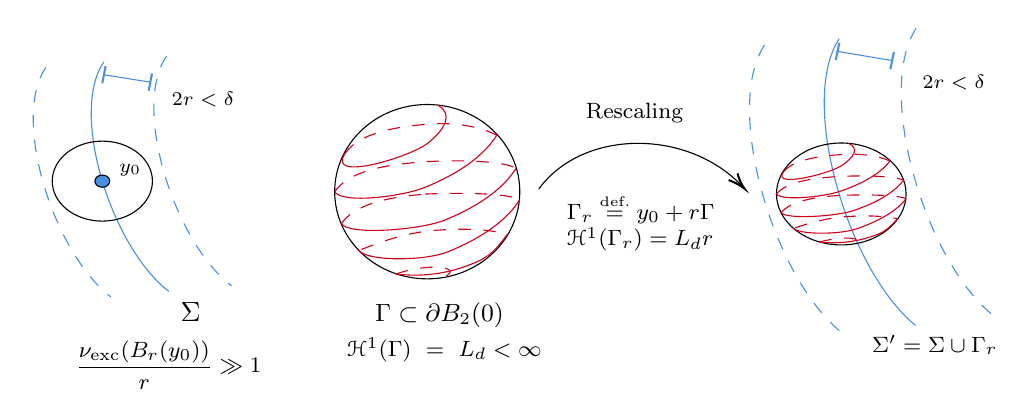
\begin{tikzpicture}[x=0.7pt,y=0.75pt,yscale=-0.75,xscale=0.85]

\draw (219,112.4) .. controls (219,81.47) and (244.16,56.4) .. (275.2,56.4) .. controls (306.24,56.4) and (331.4,81.47) .. (331.4,112.4) .. controls (331.4,143.33) and (306.24,168.4) .. (275.2,168.4) .. controls (244.16,168.4) and (219,143.33) .. (219,112.4) -- cycle ;
\draw [color={rgb, 255:red, 208; green, 2; blue, 27 } ,draw opacity=1 ] (225.29,87.89) .. controls (213.5,106.78) and (265.37,89.98) .. (275.71,81.12) .. controls (286.05,72.26) and (291.21,62.36) .. (281.62,56.85) ;
\draw [color={rgb, 255:red, 208; green, 2; blue, 27 } ,draw opacity=1 ] [dash pattern={on 4.5pt off 4.5pt}] (225.29,87.89) .. controls (234.89,73.04) and (261.53,70.34) .. (275.94,68.99) .. controls (290.35,67.64) and (307.38,70.34) .. (317.43,76.19) ;
\draw [color={rgb, 255:red, 208; green, 2; blue, 27 } ,draw opacity=1 ] (219,112.4) .. controls (223.1,120.27) and (259.79,115.77) .. (274.2,109.48) .. controls (288.61,103.18) and (307.38,92.83) .. (317.43,76.19) ;
\draw [color={rgb, 255:red, 208; green, 2; blue, 27 } ,draw opacity=1 ] [dash pattern={on 4.5pt off 4.5pt}] (219,112.4) .. controls (227.5,99.27) and (249.33,95.64) .. (264.23,94.05) .. controls (266.17,93.84) and (267.99,93.66) .. (269.65,93.51) .. controls (284.06,92.16) and (319.17,91.48) .. (329.22,97.33) ;
\draw [color={rgb, 255:red, 208; green, 2; blue, 27 } ,draw opacity=1 ] (223.1,132.87) .. controls (227.21,140.74) and (271.58,136.91) .. (285.99,130.62) .. controls (300.4,124.32) and (319.17,113.97) .. (329.22,97.33) ;
\draw [color={rgb, 255:red, 208; green, 2; blue, 27 } ,draw opacity=1 ] [dash pattern={on 4.5pt off 4.5pt}] (223.1,132.87) .. controls (231.6,119.73) and (253.43,116.11) .. (268.33,114.51) .. controls (283.23,112.92) and (272.1,114.13) .. (273.76,113.97) .. controls (275.42,113.82) and (321.36,111.73) .. (331.4,117.57) ;
\draw [color={rgb, 255:red, 208; green, 2; blue, 27 } ,draw opacity=1 ] (233.15,149.51) .. controls (237.25,157.38) and (273.76,157.16) .. (288.17,150.86) .. controls (302.58,144.56) and (321.36,134.22) .. (331.4,117.57) ;
\draw [color={rgb, 255:red, 208; green, 2; blue, 27 } ,draw opacity=1 ] [dash pattern={on 4.5pt off 4.5pt}] (235.33,149.51) .. controls (252.36,142.31) and (264.59,138.71) .. (279,137.36) .. controls (293.41,136.01) and (310.44,136.01) .. (323.98,139.61) ;
\draw [color={rgb, 255:red, 208; green, 2; blue, 27 } ,draw opacity=1 ] (256.29,165.25) .. controls (269.39,167.05) and (284.24,165.7) .. (297.34,160.75) .. controls (310.44,155.81) and (314.37,153.56) .. (323.98,139.61) ;
\draw [color={rgb, 255:red, 208; green, 2; blue, 27 } ,draw opacity=1 ] [dash pattern={on 4.5pt off 4.5pt}] (256.29,165.25) .. controls (279,157.16) and (298.21,161.65) .. (284.68,167.5) ;
\draw [color={rgb, 255:red, 74; green, 144; blue, 226 } ,draw opacity=1 ] (78.85,28.97) .. controls (68.1,45.31) and (69.38,75.83) .. (77.88,105.62) .. controls (86.08,134.36) and (101,162.44) .. (118.29,176.46) ;
\draw [color={rgb, 255:red, 74; green, 144; blue, 226 } ,draw opacity=1 ] [dash pattern={on 4.5pt off 4.5pt}] (116.89,25.4) .. controls (106.13,41.74) and (107.42,72.26) .. (115.92,102.05) .. controls (124.12,130.8) and (139.03,158.87) .. (156.33,172.89) ;
\draw [color={rgb, 255:red, 74; green, 144; blue, 226 } ,draw opacity=1 ] [dash pattern={on 4.5pt off 4.5pt}] (43.64,32.54) .. controls (32.88,48.88) and (34.17,79.39) .. (42.67,109.19) .. controls (50.87,137.93) and (65.78,166.01) .. (83.08,180.02) ;
\draw (47.46,105.62) .. controls (47.46,91.43) and (61.08,79.93) .. (77.88,79.93) .. controls (94.69,79.93) and (108.31,91.43) .. (108.31,105.62) .. controls (108.31,119.81) and (94.69,131.31) .. (77.88,131.31) .. controls (61.08,131.31) and (47.46,119.81) .. (47.46,105.62) -- cycle ;
\draw [color={rgb, 255:red, 74; green, 144; blue, 226 } ,draw opacity=1 ] (78.85,37.29) -- (107.03,42.05) ;
\draw [shift={(107.03,42.05)}, rotate = 189.59] [color={rgb, 255:red, 74; green, 144; blue, 226 } ,draw opacity=1 ][line width=0.75] (0,5.59) -- (0,-5.59) ;
\draw [shift={(78.85,37.29)}, rotate = 189.59] [color={rgb, 255:red, 74; green, 144; blue, 226 } ,draw opacity=1 ][line width=0.75] (0,5.59) -- (0,-5.59) ;
\draw [fill={rgb, 255:red, 74; green, 144; blue, 226 } ,fill opacity=1 ] (73.38,105.62) .. controls (73.38,103.45) and (75.39,101.69) .. (77.88,101.69) .. controls (80.37,101.69) and (82.39,103.45) .. (82.39,105.62) .. controls (82.39,107.79) and (80.37,109.54) .. (77.88,109.54) .. controls (75.39,109.54) and (73.38,107.79) .. (73.38,105.62) -- cycle ;
\draw [color={rgb, 255:red, 74; green, 144; blue, 226 } ,draw opacity=1 ] (525.37,14.18) .. controls (512.72,34.58) and (514.23,72.68) .. (524.23,109.87) .. controls (533.87,145.76) and (551.41,180.81) .. (571.75,198.32) ;
\draw [color={rgb, 255:red, 74; green, 144; blue, 226 } ,draw opacity=1 ] [dash pattern={on 4.5pt off 4.5pt}] (572.13,7.4) .. controls (559.48,27.8) and (561,65.9) .. (570.99,103.1) .. controls (580.64,138.99) and (598.18,174.03) .. (618.51,191.54) ;
\draw [color={rgb, 255:red, 74; green, 144; blue, 226 } ,draw opacity=1 ] [dash pattern={on 4.5pt off 4.5pt}] (479.99,18.31) .. controls (467.34,38.71) and (468.86,76.81) .. (478.85,114.01) .. controls (488.5,149.9) and (506.04,184.94) .. (526.37,202.45) ;
\draw [color={rgb, 255:red, 74; green, 144; blue, 226 } ,draw opacity=1 ] (524.4,22.25) -- (557.53,28.19) ;
\draw [shift={(557.53,28.19)}, rotate = 190.16] [color={rgb, 255:red, 74; green, 144; blue, 226 } ,draw opacity=1 ][line width=0.75] (0,5.59) -- (0,-5.59) ;
\draw [shift={(524.4,22.25)}, rotate = 190.16] [color={rgb, 255:red, 74; green, 144; blue, 226 } ,draw opacity=1 ][line width=0.75] (0,5.59) -- (0,-5.59) ;
\draw (487.3,113.87) .. controls (487.3,95.79) and (504.92,81.13) .. (526.65,81.13) .. controls (548.38,81.13) and (566,95.79) .. (566,113.87) .. controls (566,131.94) and (548.38,146.6) .. (526.65,146.6) .. controls (504.92,146.6) and (487.3,131.94) .. (487.3,113.87) -- cycle ;
\draw [color={rgb, 255:red, 208; green, 2; blue, 27 } ,draw opacity=1 ] (491.7,99.54) .. controls (483.45,110.58) and (519.76,100.76) .. (527,95.58) .. controls (534.24,90.4) and (537.86,84.62) .. (531.14,81.4) ;
\draw [color={rgb, 255:red, 208; green, 2; blue, 27 } ,draw opacity=1 ] [dash pattern={on 4.5pt off 4.5pt}] (491.7,99.54) .. controls (498.43,90.86) and (517.08,89.28) .. (527.17,88.5) .. controls (537.26,87.71) and (549.18,89.28) .. (556.22,92.7) ;
\draw [color={rgb, 255:red, 208; green, 2; blue, 27 } ,draw opacity=1 ] (487.3,113.87) .. controls (490.17,118.47) and (515.86,115.84) .. (525.95,112.16) .. controls (536.04,108.48) and (549.18,102.43) .. (556.22,92.7) ;
\draw [color={rgb, 255:red, 208; green, 2; blue, 27 } ,draw opacity=1 ] [dash pattern={on 4.5pt off 4.5pt}] (487.3,113.87) .. controls (493.25,106.19) and (508.53,104.07) .. (518.97,103.14) .. controls (520.33,103.02) and (521.6,102.92) .. (522.77,102.82) .. controls (532.86,102.04) and (557.44,101.64) .. (564.47,105.06) ;
\draw [color={rgb, 255:red, 208; green, 2; blue, 27 } ,draw opacity=1 ] (490.17,125.83) .. controls (493.05,130.43) and (524.11,128.2) .. (534.2,124.51) .. controls (544.29,120.83) and (557.44,114.79) .. (564.47,105.06) ;
\draw [color={rgb, 255:red, 208; green, 2; blue, 27 } ,draw opacity=1 ] [dash pattern={on 4.5pt off 4.5pt}] (490.17,125.83) .. controls (496.12,118.15) and (511.41,116.03) .. (521.84,115.1) .. controls (532.27,114.17) and (524.48,114.88) .. (525.64,114.79) .. controls (526.8,114.7) and (558.97,113.47) .. (566,116.89) ;
\draw [color={rgb, 255:red, 208; green, 2; blue, 27 } ,draw opacity=1 ] (497.2,135.56) .. controls (500.08,140.16) and (525.64,140.03) .. (535.73,136.35) .. controls (545.82,132.67) and (558.97,126.62) .. (566,116.89) ;
\draw [color={rgb, 255:red, 208; green, 2; blue, 27 } ,draw opacity=1 ] [dash pattern={on 4.5pt off 4.5pt}] (498.73,135.56) .. controls (510.66,131.35) and (519.22,129.25) .. (529.31,128.46) .. controls (539.4,127.67) and (551.32,127.67) .. (560.8,129.77) ;
\draw [color={rgb, 255:red, 208; green, 2; blue, 27 } ,draw opacity=1 ] (513.41,144.76) .. controls (522.58,145.81) and (532.98,145.02) .. (542.15,142.13) .. controls (551.32,139.24) and (554.08,137.92) .. (560.8,129.77) ;
\draw [color={rgb, 255:red, 208; green, 2; blue, 27 } ,draw opacity=1 ] [dash pattern={on 4.5pt off 4.5pt}] (513.41,144.76) .. controls (529.31,140.03) and (542.76,142.66) .. (533.28,146.07) ;
\draw (343,110.6) .. controls (369.73,71.99) and (433.7,71.6) .. (467,109.44) ;
\draw [shift={(468,110.6)}, rotate = 229.76] [color={rgb, 255:red, 0; green, 0; blue, 0 } ][line width=0.75] (10.93,-3.29) .. controls (6.95,-1.4) and (3.31,-0.3) .. (0,0) .. controls (3.31,0.3) and (6.95,1.4) .. (10.93,3.29) ;

\draw (123.77,181.94) node [anchor=north west][inner sep=0.75pt] {$\Sigma $};
\draw (118.14,46.97) node [anchor=north west][inner sep=0.75pt] [font=\scriptsize,xslant=-0.05] {$2r< \delta $};
\draw (86.46,92.79) node [anchor=north west][inner sep=0.75pt] [font=\scriptsize] {$y_{0}$};
\draw (60,206.4) node [anchor=north west][inner sep=0.75pt] [font=\footnotesize] {$
\displaystyle \frac{\nuexc(B_{r}(y_{0}))}{r} \gg 1$};
\draw (543.85,202.87) node [anchor=north west][inner sep=0.75pt] [font=\footnotesize] {$\Sigma '=\Sigma \cup \Gamma _{r}$};
\draw (574.08,35.47) node [anchor=north west][inner sep=0.75pt] [font=\scriptsize,xslant=-0.05] {$2r< \delta $};
\draw (242,182) node [anchor=north west][inner sep=0.75pt] [font=\footnotesize] [align=left] {{\small $\displaystyle \Gamma \subset \partial B_{2}( 0)$}};
\draw (225,204.4) node [anchor=north west][inner sep=0.75pt] [font=\footnotesize] {$\cH^{1}( \Gamma ) \ =\ L_{d} < \infty $};
\draw (350,112.4) node [anchor=north west][inner sep=0.75pt] [font=\footnotesize] {$ \begin{array}{l}
\Gamma _{r} \eqdef y_{0} +r\Gamma \\
\cH^{1}( \Gamma _{r}) = L_{d} r
\end{array}$};
\draw (370,54) node [anchor=north west][inner sep=0.75pt] [align=left] {{\footnotesize Rescaling}};
\end{tikzpicture}
\caption{Scheme of the proof of Theorem \ref{theorem.solutions_are_absolutely_continuous}. For the new competitor, created with the curve $\Gamma$ from Lemma~\ref{lemma.curve_on_B2}, we~pay a little more in the transportation cost to generate $\alpha^{-1}\cH^1\mres \Gamma_r$, but pay much less by projecting the remaining mass onto it.}\label{figure.L_infty_bounds}
\end{figure}

\begin{theorem}\label{theorem.solutions_are_absolutely_continuous}
Given $\rho_0 \in \mathcal{P}_p(\RR^d)$, let $\nu$ be a solution to \eqref{problem.shape_optimization_relaxed}.
Then it holds that the measures $\left(\nu_\delta\right)_{\delta > 0}$ are of the form
\[
\nu_\delta = \theta_\delta \cH^1\mres \Sigma,
\quad\text{with $
\norm{\theta_\delta}_{L^\infty(\Sigma, \cH^1)}
\le
\frac{7}{2}\frac{C_d}{\mathcal{L}(\nu)}$,}
\]
for $C_d = 2 + \cH^1(\Gamma_d)$, $\Gamma_d$ being the set from Lemma \ref{lemma.curve_on_B2}.

Therefore,
if $\rho_0 \ll \cH^1$ or has a $L^{\infty}$ density with respect to $\cH^1$, so~does $\nu$, in~particular it is a rectifiable measure.
\end{theorem}

\begin{proof}
For $y_0 \in \Sigma$, let us define the one-dimensional upper density~\cite[Def.\,2.55]{ambrosio2000functions}
\begin{equation*}
\theta_\delta(y_0)\eqdef\limsup_{r \to 0} \frac{\nu_{\delta}(B_r)}{2r}.
\end{equation*}
We will show that $\theta_{\delta}(y_0)\leq \frac{7}{2}\sfrac{C_d}{\cL(\nu)}$, so~that thanks to~\cite[Th.\,2.56]{ambrosio2000functions}, $\nu_\delta \ll \cH^1\mres\Sigma$.
Since $\Sigma$ is 1-rectifiable, it follows that for $\cH^1$-a.e.~$y_0 \in \Gamma$, $\theta_\delta(y_0)$ is the Radon-Besicovitch
derivative of $\nu_\delta$ with respect to $\cH^1\mres\Sigma$, and the claim of the theorem follows.

From the optimality of $\nu$, the measure $\nu_{\delta,r}$ solves problem \eqref{auxiliary_problem}. In order to build a competitor we consider the set $\Gamma_d$ from Lemma \ref{lemma.curve_on_B2}, choose some point $\bar y \in \Gamma_d$ and define
\[
\Gamma_r
\eqdef
[y_0, y_0 + r\bar y]\cup
(y_0 + r\Gamma_d),
\]
which is contained in $\overline{B}_{2r}(y_0)$. Notice that $\Sigma \cup \Gamma_{r}$ is always a compact, connected and $1$-rectifiable set and one has
\[
\cH^1(\Gamma_{r})
=
C_dr,
\]
where $C_d = 1 + \cH^1(\Gamma_d)$ is a constant depending only on the dimension.

In the sequel, setting $\alpha = \mathcal{L}(\nu)$ we define the following parameter
\[
m_{r} \eqdef
\frac{\cH^1(\Gamma_r)}{\alpha \nu_\delta(B_r)}.\]
Suppose that $C_d/\alpha < 2\theta_{\delta}(y_0)$. Then,
\begin{equation*}
1> m_0\eqdef\frac{C_d}{2\alpha\theta_\delta(y_0)}= \liminf_{r \to 0} m_r.
\end{equation*}
Now, we~consider a subsequence $(r_{k})_{k\in \mathbb{N}}\searrow 0$ such that $\lim_{k \to \infty} m_{r_k}=\liminf_{r \to 0} m_r$. In particular, $m_{r_k} \in (0,1)$ for $r_k$ sufficiently small.
For simplicity, in the sequel, we~drop the subscript $k$, yet we consider only $r \in \{r_{k}\}_{k\in \mathbb{N}}$.

Let $\gamma_{\Gamma_{r}}$ be an optimal transport plan between $m_r\rho_{\delta, r}$ and $\alpha^{-1}\cH^1\mres \Gamma_{r}$ for the Wasserstein-$p$ distance and define the new plan
\[
\tilde \gamma_{\delta, r}
\eqdef
\gamma_{\Gamma_{r}}
+
(1-m_{r})
\left(
\text{id},
\pi_{\Gamma_{r}}
\right)_\sharp
\rho_{\delta, r},
\text{ and }
\tilde\nu_{\delta, r}
\eqdef {\pi_{1}}_\sharp \tilde \gamma_{\delta, r},
\]
where $\pi_{\Gamma_{r}}$ is a measurable selection of the projection operator onto $\Gamma_{r}$. This construction is illustrated in Figure~\ref{figure.L_infty_bounds}. Therefore $\tilde\nu_{\delta, r}$ is admissible for \eqref{auxiliary_problem} and we have the following estimate:
\begin{equation*}
W_p^p(\rho_{\delta, r}, \tilde\nu_{\delta, r})
\le
\int_{\RR^d\times \RR^d} |x - y|^p\dd \gamma_{\Gamma_{r}}
+
(1 - m_{r})\int_{\RR^d} \dist(x, \Gamma_r)^p\dd \rho_{\delta,r}.
\end{equation*}

We will estimate each term of the previous inequality separately. For the first one, notice that as $\supp \gamma_{\Gamma_{r}} \subset \Pi_{\Sigma}^{-1}(B_r(y_0)) \times \overline{B}_{2r}(y_0)$, it holds that:
\[
|x - y| \le \dist(x,\Sigma) + 3r, \quad \text{ for $\gamma_{\Gamma_{r}}$-a.e.\ $(x,y)$}.
\]
For the second term, as the projection of $x$ onto $\Sigma$ is inside $B_r(y_0)$, if follows from Lemma \ref{lemma.curve_on_B2} that:
\[
\dist(x, \Gamma_r) \le \dist(x, \Sigma) - \frac{r}{2}, \quad\text{for } \dist(x, \Sigma) > 2r.
\]
Therefore, for a fixed $\delta$ and taking $2r < \delta$, the Wasserstein distance is bounded by:
\[
W_p^p(\rho_{\delta, r}, \tilde\nu_{\delta, r})
\le
m_{r}
\int_{\RR^d}\hspace*{-1mm}
(\dist(x,\Sigma) + 3r)^p\dd \rho_{\delta,r}
+
(1 - m_{r})
\int_{\RR^d}\hspace*{-1mm}
(\dist(x, \Sigma) - r/2)^p\dd \rho_{\delta,r}.
\]

Notice that
$
W_p^p(\rho_{\delta, r},\nu_{\delta, r})
=
\int_{\RR^d} \dist(x,\Sigma)^p\dd \rho_{\delta,r},
$
so in order to compare the Wasserstein distances we use the following inequalities:
\begin{align*}
\left(\dist(x,\Sigma) + 3r\right)^p
&\le
\dist(x,\Sigma)^p
+
3rp
(\dist(x,\Sigma)+3r)^{p-1}, \\
\left(\dist(x,\Sigma) -\frac{r}{2}\right)^p
&\le
\dist(x,\Sigma)^p
-
\frac{r}{2}p
\Bigl(\dist(x,\Sigma)-\frac{r}{2}\Bigr)^{p-1},
\end{align*}
which follow from the convexity of $t\mto |t|^p$.
Then, given $\varepsilon>0$, if $r\le \delta\varepsilon$ one deduces,
for $\dist(x,\Sigma)\ge \delta$, that:
\begin{align*}
\left(\dist(x,\Sigma) + 3r\right)^p
&\le
\dist(x,\Sigma)^p
+
3 r p(1+3\varepsilon)^{p-1}
\dist(x,\Sigma)^{p-1}, \\
\left(\dist(x,\Sigma) -\frac{r}{2}\right)^p
&\le
\dist(x,\Sigma)^p
-
\frac{r}{2}p \left(1-\frac{\varepsilon}{2}\right)^{p-1}
\dist(x,\Sigma)^{p-1}.
\end{align*}
Therefore it holds that
\begin{align*}
W_p^p(\rho_{\delta, r}, \tilde\nu_{\delta, r})
&\le
W_p^p(\rho_{\delta, r}, \nu_{\delta, r})
+
pr\Delta_{r,\varepsilon}
\int_{\RR^d}
\dist(x,\Sigma)^{p-1}\dd \rho_{\delta,r}\\
\text{ for }
\Delta_{r,\varepsilon}
&=
3m_{r}
\left(
1 + 3\varepsilon
\right)^{p-1}
-
\frac{1 - m_r}{2}
\Bigl(
1 - \frac{\varepsilon}{2}
\Bigr)^{p-1}.
\end{align*}
Hence from the optimality of $\nu_{\delta,r}$ we have $\Delta_{r,\varepsilon} \ge 0$, so~that letting $r \to 0$ and then $\varepsilon\to 0$, it must hold that
$3 m_0\ge (1-m_0)/2$, that is:
\[
\theta_\delta(y_0)
\le
\frac{7}{2}\frac{C_d}{\alpha}.
\]
As a result, the family $\left(\nu_\delta\right)_{\delta > 0}$ has a uniform $L^\infty$ density bounds, and so does the limit measure $\sup_{\delta > 0} \nu_\delta = \left(\sup_{\delta > 0}\theta_\delta\right)\cH^1\mres \Sigma$. But as the exceeding measure can be decomposed as~\eqref{nuexc.further_decomposition} we deduce that
whenever the initial measure $\rho_0 \ll \cH^1$ or has a~$L^{\infty}$ density with respect to $\cH^1$, so~does the solution $\nu$.
\end{proof}

\section{Existence of solutions to \texorpdfstring{\eqref{problem.shape_optimization}}{eqref}}\label{section.blowup}
This section is dedicated to the proof of~Theorem \ref{theorem.the_big_one}, item~(2). Knowing
that the excess measure is absolutely continuous (Theorem~\ref{theorem.solutions_are_absolutely_continuous}), we~use
a blow up argument near a rectifiability point $y_0$ of $\Sigma$.
From~Lemma \ref{lemma.auxiliary_problem}, the blow-ups of $\nuexc$ minimize a family of functionals $(F_r)_{r > 0}$, which in turn $\Gamma$-converge to some functional $F$.
Since these blow-ups also converge (for $\cH^1$-a.e.~$y_0$) to a uniform density on $T_{y_0}\Sigma$, this limit measure must also minimize the $\Gamma$-limit $F$.
Yet if it is not zero, we~can build a better competitor (Lemma~\ref{lemma.better_competitor} below), giving a contradiction to the minimality of the uniform measure. We~deduce that $\nuexc$ vanishes.

\subsection{Blow-up and $\Gamma$-convergence}\label{sec.gamma_convergence}
In the sequel, we~assume that $\rho_0 \ll \mathcal{H}^1$, so~that from Theorem~\ref{theorem.solutions_are_absolutely_continuous} any minimizer $\nu$, as well as ${(\nu_\delta)}_{\delta > 0}$ (defined in~\eqref{measure_nu_delta}), are rectifiable measures and we can write
\[
\nu_\delta = \theta_\delta \mathcal{H}^1\mres \Sigma,
\text{ for }
\theta_\delta \in L^1(\cH^1\mres \Sigma).
\]

Observe that $\nu_\delta$-a.e.~$y \in \Sigma$ is a rectifiability point, and we choose $y_0 \in \Sigma$ such that
\begin{equation}\label{y0fixed_for_blowup}
T_{y_0}\Sigma \text{ exists }
\quad\text{ and } \quad
y_0 \text{ is a Lebesgue point of }
\theta_\delta.
\end{equation}
We then use Lemma~\ref{lemma.auxiliary_problem} with the choice $\mathcal{S}_0\times \mathcal{S}_1 = D_{\delta}\times B_r(y_0)$, and we focus on the variational problem~\eqref{auxiliary_problem_sigma}: we obtain the families of measures $\left(\nu_{\delta ,r}\right)_{r > 0}$ and $\left(\sigma_{\delta ,r}\right)_{r > 0}$ as $\nu_{\delta ,r} \eqdef \nu_\delta \mres B_r(y_0)$ and $\sigma_{\delta ,r} \eqdef {\pi_{(1-r)}}_\sharp\gamma_{\delta,r}$, where $\left(\sigma_{\delta,t}\right)_{t \in [0,1]}$ is a family of geodesic interpolations, as in Lemma~\ref{lemma.auxiliary_problem}, so~that
\begin{equation}\label{auxiliary_problem_geodesic}
\nu_{\delta ,r}
\in
\argmin
\left\{
W_p^p\left(
\sigma_{\delta ,r}, \nu'
\right) :
\begin{array}{c}
\text{there exists $\Gamma$ such that}\\
\nu' \in \mathcal{M}_+(\Sigma \cup \Gamma),\\
\nu' \ge \alpha^{-1}\mathcal{H}^1\mres \left(\Gamma\setminus \Sigma\right), \\
\Sigma \cup \Gamma \in \mathcal{A}, \
\nu'(\RR^d) = \nu_{\delta ,r}(\RR^d)
\end{array}
\right\}.
\end{equation}
From Lemma~\ref{lemma.minimal_distance2Sigma} the optimal transport plan between $\nu_{\delta ,r}$ and $\sigma_{\delta ,r}$ is supported on $\text{graph}(\Pi_\Sigma)$.

The sequence of measures $\nu_{\delta ,r}$ are essentially a localization of $\nu_\delta$ around $y_0$ so, by~the blow-up theorem \ref{theorem.rectifiability_tangentiability} (see also~\cite[Th.\,2.83]{ambrosio2000functions}), it holds that
\begin{equation}\label{blowup_measures_nu}
r^{-1}\Phi^{y_0,r}_{\sharp}\nu_{\delta ,r} \xrightharpoonup[r \to 0]{\ts\star}
\theta_\delta(y_0)\mathcal{H}^1\mres [-\tau, \tau],
\quad\text{where $\RR\tau = T_{y_0}\Sigma$.}
\end{equation}
Up to a subsequence (not labeled) we also have:
\begin{equation}\label{blowup_measures_sigma}
r^{-1}\Phi^{y_0,r}_{\sharp}\sigma_{\delta ,r} \xrightharpoonup[r \to 0]{\ts\star}
\bar \sigma_{\delta}
\end{equation}
for some measure $\bar \sigma_{\delta}$.
By construction $\sigma_{\delta ,r}$ is supported on $\{r\delta^{-1}\ge\dist(\cdot,\Sigma)\ge r\delta\}$, so~that $\supp \bar \sigma_{\delta} \subset \{x : \delta^{-1} \ge \dist(x,\RR\tau) \ge \delta \}$.

In view of~\eqref{blowup_measures_nu} and~\eqref{blowup_measures_sigma}, we~introduce the blow-ups of the measures $\nu_{\delta ,r}$ and $\sigma_{\delta , r}$,
\begin{equation}\label{blowup_measures_renormalized}
\bar\nu_{\delta ,r}
\eqdef
\frac{1}{r}\,
\Phi^{y_0,r}_{\sharp}
\nu_{\delta ,r},
\quad
\bar\sigma_{\delta ,r}
\eqdef
\frac{1}{r}\,\Phi^{y_0,r}_{\sharp}
\sigma_{\delta , r},
\text{ and the set }
\Sigma_r \eqdef
\frac{\Sigma - y_0}{r}\cap \overline{B_1(0)}.
\end{equation}

In addition, we~define a family of functionals ${\left(F_r\right)}_{r > 0}$ as
\begin{equation}\label{family_Fr}
F_r(\nu') \eqdef
\begin{cases}
W_p^p\left(
\bar \sigma_{\delta ,r},
\nu'
\right),&
\begin{array}{c}
\text{there exists $\Gamma \subset \overline{B_1(0)}$ such that}\\
\nu' \in \mathcal{M}_+(\Sigma_r \cup \Gamma), \
\nu' \ge \alpha^{-1}\cH^1\mres(\Gamma\setminus \Sigma_r),\\
\Bigl(\dfrac{\Sigma-y_0}{r}\Bigr) \cup \Gamma \text{ closed and connected}, \\
\nu'(\overline{B_1(0)}) = \dfrac{\nu_\delta(B_r(y_0))}{r},
\end{array} \\
+\infty,& \text{ otherwise,}
\end{cases}
\end{equation}
where $\alpha = \mathcal{L}(\nu)$.
Observing that for any given measures $\mu', \nu'$ we have:
\begin{equation}\label{blowup_Wasserstein_identity}
W_p^p
\Bigl(
\frac{1}{r}\,\Phi^{y_0, r}_\sharp \mu',
\frac{1}{r}\,\Phi^{y_0, r}_\sharp \nu'
\Bigr)
=
\frac{1}{r^{p+1}}\,
W_p^p( \mu', \nu').
\end{equation}
and recalling
\eqref{auxiliary_problem_geodesic},
we see that $\bar \nu_{\delta ,r} \in \argmin F_r$ for any $r>0$.

The natural candidate for the limit of this family is the following:
\begin{equation}\label{Gamma_limitF}
F(\nu') \eqdef
\begin{cases}
W_p^p\left( \bar \sigma_{\delta}, \nu' \right),&
\begin{array}{c}
\text{there exists $\Gamma \subset \overline{B_1(0)}$ such that}\\
\nu' \in \mathcal{M}_+\left([-\tau, \tau] \cup \Gamma\right),
\\ \nu' \ge \alpha^{-1}\cH^1\mres \left(\Gamma\setminus[-\tau,\tau]\right),\\
\RR\tau \cup \Gamma \text{ closed and connected},\\ \nu'(\overline{B_1(0)}) = 2\theta_\delta(y_0),
\end{array} \\
+\infty,& \text{ otherwise.}
\end{cases}
\end{equation}
We prove in Theorem~\ref{theorem.Gamma_convergence} below that $F_r$ $\Gamma$-converges to $F$ as $r\to 0^+$. We~refer to~\cite{dal_maso_introduction_1993,braides_gamma-convergence_2002} and in particular to~\cite[Def.\,1.24]{braides_gamma-convergence_2002}) for the definition of the (lower and upper) $\Gamma$-limit. From the properties of the $\Gamma$-convergence, see~\cite[Cor.\,7.20]{dal_maso_introduction_1993}, it follows that $\theta_\delta(y_0)\cH^1\mres [-\tau, \tau]$ must be a minimizer of $F$ (as the limit of minimizers of $F_r$). The estimate from below of the $\Gamma$-liminf is obtained with the tools developed so far, while estimating the $\Gamma$-limsup will require an appropriate construction illustrated in Figure~\ref{figure.gamma_convergence}.

\begin{figure}[t]
\centering

\resizebox{1\linewidth}{!}{%
\tikzset{every picture/.style={line width=0.75pt}}
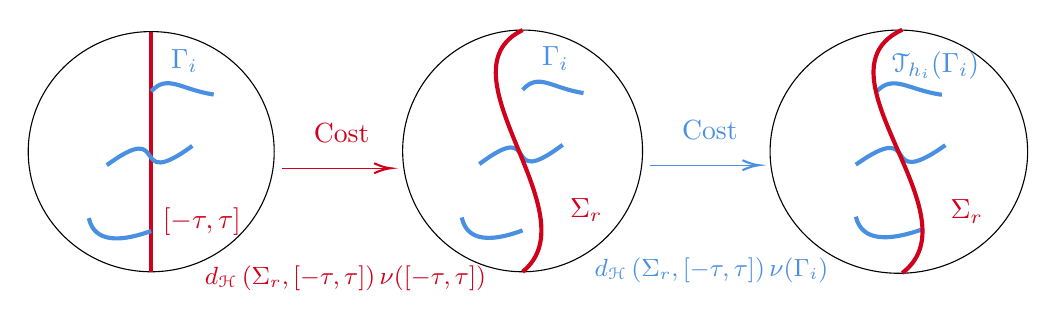
\begin{tikzpicture}[x=0.55pt,y=0.55pt,yscale=-1,xscale=1]
\centering

\draw (1.6,80.3) .. controls (1.6,36.72) and (37.78,1.4) .. (82.4,1.4) .. controls (127.02,1.4) and (163.2,36.72) .. (163.2,80.3) .. controls (163.2,123.88) and (127.02,159.2) .. (82.4,159.2) .. controls (37.78,159.2) and (1.6,123.88) .. (1.6,80.3) -- cycle ;
\draw (247.6,79.8) .. controls (247.6,35.95) and (282.88,0.4) .. (326.4,0.4) .. controls (369.92,0.4) and (405.2,35.95) .. (405.2,79.8) .. controls (405.2,123.65) and (369.92,159.2) .. (326.4,159.2) .. controls (282.88,159.2) and (247.6,123.65) .. (247.6,79.8) -- cycle ;
\draw (489,80.31) .. controls (489,36.18) and (526.88,0.41) .. (573.6,0.41) .. controls (620.32,0.41) and (658.2,36.18) .. (658.2,80.31) .. controls (658.2,124.43) and (620.32,160.2) .. (573.6,160.2) .. controls (526.88,160.2) and (489,124.43) .. (489,80.31) -- cycle ;
\draw [color={rgb, 255:red, 208; green, 2; blue, 27 } ,draw opacity=1 ][line width=1.5] (82.4,1.4) -- (82.4,159.2) ;
\draw [color={rgb, 255:red, 74; green, 144; blue, 226 } ,draw opacity=1 ][line width=1.5] (53.23,89.16) .. controls (96.44,57.52) and (66.2,108.15) .. (109.41,76.5) ;
\draw [color={rgb, 255:red, 74; green, 144; blue, 226 } ,draw opacity=1 ][line width=1.5] (41.35,123.97) .. controls (43.51,132.41) and (49.99,144.01) .. (82.4,132.41) ;
\draw [color={rgb, 255:red, 74; green, 144; blue, 226 } ,draw opacity=1 ][line width=1.5] (82.4,40.64) .. controls (93.2,29.04) and (101.84,39.58) .. (123.45,42.75) ;
\draw [color={rgb, 255:red, 74; green, 144; blue, 226 } ,draw opacity=1 ][line width=1.5] (297.96,88.5) .. controls (340.1,56.66) and (310.6,107.61) .. (352.74,75.77) ;
\draw [color={rgb, 255:red, 74; green, 144; blue, 226 } ,draw opacity=1 ][line width=1.5] (286.37,123.53) .. controls (288.47,132.03) and (294.8,143.7) .. (326.4,132.03) ;
\draw [color={rgb, 255:red, 74; green, 144; blue, 226 } ,draw opacity=1 ][line width=1.5] (326.4,39.68) .. controls (336.93,28) and (345.36,38.61) .. (366.43,41.8) ;
\draw [color={rgb, 255:red, 208; green, 2; blue, 27 } ,draw opacity=1 ][line width=1.5] (326.4,0.4) .. controls (269.51,28.21) and (372.75,121.62) .. (326.4,159.2) ;
\draw [color={rgb, 255:red, 74; green, 144; blue, 226 } ,draw opacity=1 ][line width=1.5] (545.32,88.85) .. controls (590.57,56.81) and (558.9,108.08) .. (604.14,76.03) ;
\draw [color={rgb, 255:red, 74; green, 144; blue, 226 } ,draw opacity=1 ][line width=1.5] (545.32,123.03) .. controls (547.59,131.58) and (554.37,143.32) .. (588.3,131.58) ;
\draw [color={rgb, 255:red, 74; green, 144; blue, 226 } ,draw opacity=1 ][line width=1.5] (558.9,40.79) .. controls (570.21,29.04) and (579.26,39.72) .. (601.88,42.92) ;
\draw [color={rgb, 255:red, 208; green, 2; blue, 27 } ,draw opacity=1 ][line width=1.5] (575.86,0.2) .. controls (514.79,28.18) and (625.63,122.18) .. (575.86,159.99) ;
\draw [color={rgb, 255:red, 208; green, 2; blue, 27 } ,draw opacity=1 ] (168.4,91.2) -- (237.8,91.2) ;
\draw [shift={(239.8,91.2)}, rotate = 180] [color={rgb, 255:red, 208; green, 2; blue, 27 } ,draw opacity=1 ][line width=0.75] (10.93,-3.29) .. controls (6.95,-1.4) and (3.31,-0.3) .. (0,0) .. controls (3.31,0.3) and (6.95,1.4) .. (10.93,3.29) ;
\draw [color={rgb, 255:red, 74; green, 144; blue, 226 } ,draw opacity=1 ] (410.4,89.2) -- (479.8,89.2) ;
\draw [shift={(481.8,89.2)}, rotate = 180] [color={rgb, 255:red, 74; green, 144; blue, 226 } ,draw opacity=1 ][line width=0.75] (10.93,-3.29) .. controls (6.95,-1.4) and (3.31,-0.3) .. (0,0) .. controls (3.31,0.3) and (6.95,1.4) .. (10.93,3.29) ;

\draw (93.72,11.43) node [anchor=north west][inner sep=0.75pt] [font=\normalsize,color={rgb, 255:red, 74; green, 144; blue, 226 } ,opacity=1 ] {$\Gamma _{i}$};
\draw (88.29,115.11) node [anchor=north west][inner sep=0.75pt] [font=\normalsize,color={rgb, 255:red, 208; green, 2; blue, 27 } ,opacity=1 ] {$[ -\tau ,\tau ]$};
\draw (355.88,109.37) node [anchor=north west][inner sep=0.75pt] [font=\normalsize,color={rgb, 255:red, 208; green, 2; blue, 27 } ,opacity=1 ] {$\Sigma _{r}$};
\draw (337.45,9.81) node [anchor=north west][inner sep=0.75pt] [font=\normalsize,color={rgb, 255:red, 74; green, 144; blue, 226 } ,opacity=1 ] {$\Gamma _{i}$};
\draw (567.24,12.62) node [anchor=north west][inner sep=0.75pt] [font=\normalsize,color={rgb, 255:red, 74; green, 144; blue, 226 } ,opacity=1 ] {$\mathcal{T}_{h_{i}}( \Gamma _{i})$};
\draw (187.5,60.01) node [anchor=north west][inner sep=0.75pt] [color={rgb, 255:red, 208; green, 2; blue, 27 } ,opacity=1 ] [align=left] {Cost};
\draw (116,153.8) node [anchor=north west][inner sep=0.75pt] [font=\small,color={rgb, 255:red, 208; green, 2; blue, 27 } ,opacity=1 ] {$\distH\left(\Sigma_{r} ,[ -\tau ,\tau ]\right) \nu ([ -\tau ,\tau ])$};
\draw (372,148.4) node [anchor=north west][inner sep=0.75pt] [font=\small,color={rgb, 255:red, 74; green, 144; blue, 226 } ,opacity=1 ] {$\distH\left(\Sigma_{r} ,[ -\tau ,\tau ]\right) \nu ( \Gamma _{i})$};
\draw (429.5,58.01) node [anchor=north west][inner sep=0.75pt] [color={rgb, 255:red, 74; green, 144; blue, 226 } ,opacity=1 ] [align=left] {Cost};
\draw (605.88,110.37) node [anchor=north west][inner sep=0.75pt] [font=\normalsize,color={rgb, 255:red, 208; green, 2; blue, 27 } ,opacity=1 ] {$\Sigma _{r}$};
\end{tikzpicture}
}
\caption{Transportation argument for the construction of a recovery sequence in the $\Gamma$ convergence of $(F_r)_{r>0}$. Both operations have a transportation cost of the order $\distH\left(\Sigma_r ,[ -\tau ,\tau ]\right)$, and hence converge to $0$.}\label{figure.gamma_convergence}
\end{figure}

\begin{theorem}\label{theorem.Gamma_convergence}
The family of functionals ${\left(F_r\right)}_{r > 0}$ $\Gamma$-converges to $F$ as $r\to 0^+$, in~the narrow topology.
\end{theorem}

\begin{proof}

$\Gamma$-liminf: we consider an infinitesimal sequence $(r_n)_{n \in \mathbb{N}}$ such that ${(\nu_{n}')}_{n \in \mathbb{N}}$ converges to $\nu'$ in the narrow
sense in $\overline{B_1(0)}$, and that $\liminf_{n \to \infty} F_{r_n}(\nu_n') < \infty$ for all $n \in \mathbb{N}$, otherwise there is nothing to prove.

First we look at the first marginals in the definition of $F_{r_n}$. From~\eqref{blowup_measures_sigma} we know that $\bar \sigma_{\delta, r_n}\xrightharpoonup[n \to \infty]{\star} \bar\sigma_{\delta}$.
By the lower semi-continuity of the Wasserstein distance with respect to the narrow convergence,
if we prove that $F(\nu') < \infty$, that is, if the limit satisfies the constraints in the definition of $F$, we~will have
\[
F(\nu') \le \liminf_{n \to \infty} F_{r_n}(\nu_n').
\]

As $\alpha \nu_n' \ge \cH^1\mres \left(\Gamma_{n}\setminus\Sigma_{r_n}\right)$ for some $\Gamma_n \subset \overline{B_1(0)}$ such that $r_n^{-1}(\Sigma-y_0)\cup \Gamma_n \in \mathcal{A}$, Blaschke's theorem~\cite[Th.\,6.1]{ambrosio2000functions}
and Lemma~\ref{lemma.blowup_domain_measure} imply that, up to a subsequence, $\Gamma_n \xrightarrow[n \to \infty]{\distH} \Gamma$ for some closed set $\Gamma \subset \overline{ B_1(0)}$ and $r_n^{-1}(\Sigma-y_0)\,{\xrightarrow[n \to \infty]{K}}\, \RR\tau$. Hence,
\[
\Xi_n
\eqdef
\Bigl(
\frac{\Sigma - y_0}{r_n}
\Bigr)
\cup \Gamma_n
\xrightarrow[n \to \infty]{\ts K}
\Xi
\eqdef
\RR\tau \cup \Gamma.
\]

Let us check that $\Xi$ is connected (which is not immediate since the Kuratowski limit of connected sets is not necessarily connected).
Assume by contradiction that there are two disjoint open sets $U,V \subset \RR^d$ such that $U\cap \Xi$ and $V\cap \Xi$ form a partition of $\Xi$. Since $\RR\tau \subset \Xi$ is connected, it is contained in either $U$ or $V$ (say, $U$). As a result, $V\cap \Xi\subset \Gamma \subset \overline{B_1(0)}$ is bounded, and possibly replacing $V$ with $V\cap B_2(0)$, we~may assume that $V$ is bounded too, so~that $\partial V$ is compact.
Since $\Xi\subset V\cap (\RR^d\setminus \overline{V})$, we~note that $\partial V \cap \Xi=\emptyset$, and we deduce that $\min_{x\in \partial V} \dist(x,\Xi)>0$.

Now, the Kuratowski convergence of $\Xi_n$ towards $\Xi$ implies that, for all $n$ large enough, $\Xi_n$ intersects both $V$ and $U\subset \RR^d\setminus \overline{V}$, hence, by the connectedness of $\Xi_n$, there exists $x_n\in \Xi_n \cap \partial V$.
But the Kuratowski convergence also implies that $\dist(\cdot,\Xi_n) \xrightarrow[]{} \dist(\cdot,\Xi)$ locally uniformly (hence uniformly on $\partial V$), which contradicts that $\min_{x\in \partial V} \dist(x,\Xi)>0$. As a result, $\Xi$ is connected.

The fact that $\supp\nu' \subset [-\tau, \tau]\cup \Gamma$ comes from the weak convergence of~$\nu_{n}'$ to~$\nu'$. As this convergence takes place in a compact set it also holds that $\nu'(\overline{B_1(0)}) = \lim_{n \to \infty} \nu_{n}'(\overline{B_1(0)}) = 2\theta_\delta(y_0)$ since $\theta_\delta(y_0)$ is the density of $\nu_\delta$ at $y_0$.

It only remains to verify the density constraints, $\alpha \nu' \ge \mathcal{H}^1\mres \left(\Gamma\setminus [-\tau,\tau]\right)$. We~cannot apply \Golab's theorem to $\nu_n'$ since, although $\alpha\nu_n' \ge \cH^1\mres \left( \Gamma_n\setminus \Sigma_{r_n}\right)$, we~do not have an upper bound on the number of connected components of $\Gamma_n\setminus \Sigma_{r_n}$. What we do know is that the sequence $\Xi_n = r_n^{-1}(\Sigma - y_0) \cup \Gamma_n$ satisfies the assumptions of Theorem \ref{theorem.Golab_localversion},
so we apply it to the measures $\cH^1\mres\Xi_n$ instead, remembering that
\begin{equation*}
\mathcal{H}^1\mres
\Bigl(
\frac{\Sigma - y_0}{r_n}
\Bigr)
+
\alpha\nu_n'
\ge
\mathcal{H}^1\mres
\Bigl(
\frac{\Sigma - y_0}{r_n}\cup\Gamma_n
\Bigl).
\end{equation*}
The left-hand side converges in the local weak-$\star$ sense to
$\cH^1\mres \RR\tau + \alpha\nu'$. The right-hand side
(which is bounded by the left-hand side)
converges in the same sense, up to a subsequence. We~let
$\lambda$ denote a limit and Theorem~\ref{theorem.Golab_localversion} implies that $\lambda \ge \cH^1\mres (\RR\tau\cup \Gamma)$, which gives
$
\cH^1\mres \RR\tau + \alpha\nu' \ge \cH^1\mres (\RR\tau\cup \Gamma),
$
and thus
\[
\alpha\nu' \ge \cH^1\mres(\Gamma\setminus [-\tau,\tau]).
\]

\par $\Gamma$-limsup: Let $(r_{n})_{n\in\mathbb{N}}$ be an infinitesimal sequence. By Lemma~\ref{lemma.blowup_domain_measure}, we~know that $(\Sigma-y_0)/r_{n}$ converges in the Kuratowski sense towards $\RR\tau$, and $\Sigma_{r_n}\eqdef (\Sigma-\nobreak y_0)/r_{n}\cap\nobreak\overline{B_1(0)}$ converges towards $[-\tau,\tau]$ for the Hausdorff distance.

The strategy to prove the limsup is illustrated in Figure~\ref{figure.gamma_convergence},
and roughly explained as follows. We~concatenate three steps. First we renormalize $\nu'$ to satisfy the mass constraint in $F_{r_{n}}$. But this normalization may break the condition $\alpha \nu_n'\ge \cH^1\mres \left(\Gamma\setminus [-\tau,\tau]\right)$, so~we slightly shrink the support to satisfy this constraint again. We~also need the measure $\nu_{n}'$ to be supported on some connected set $\Sigma_{r_{n}}\cup \Gamma_{n}$, hence we move the mass of $\nu'$ from $[-\tau,\tau]$ to $\Sigma_{r_n}$ by projection, and we translate the mass of each connected component of the (shrunk) $\Gamma\setminus [-\tau,\tau]$ so that it is connected to $\Sigma_{r_n}$. Eventually, by doing so, some parts of the support may get out of $\overline{B_1(0)}$, so~we project the residual mass onto $\overline{B_1(0)}$.

To be more precise, we~first address the case $\theta_\delta(y_0)=0$. As $F(\nu')<+\infty$ if and only if $\nu'=0$, we~need only prove the result for $\nu'=0$. Let $P_n$ be any measurable selection of the projection onto ${\Sigma_{r_n}}$, and define $\nu_n'\eqdef {P_n}_{\sharp} \bar \sigma_{\delta, r_n}$. With $\Gamma=\emptyset$, and since $\abs{x-P_n(x)}\le \delta^{-1}$ for all $x\in \supp \bar \sigma_{\delta,r_n}$, we~observe that:
\[
F_{r_n}(\nu'_n)\le W_p^p(\bar \sigma_{\delta, r_n},\nu_n')\le \delta^{-p} \frac{\nu_\delta(B_{r_n})}{r_n} \xrightarrow[n\to +\infty]{} 0 = F(\nu').
\]
Moreover, as $\nu'_n \xrightharpoonup[n \to +\infty]{} \nu'$ in the narrow topology, we~have built a recovery sequence for $\nu'$.

Now, we~deal with the case $\theta_{\delta}(y_0)>0$. Let $\nu'$ such that $F(\nu') < +\infty$, and let $\Gamma$ be a set as in~\eqref{Gamma_limitF}. Observe that $[-\tau,\tau]\cup \Gamma$ is connected, being the projection of $\RR\tau\cup \Gamma$ onto $\overline{B_1(0)}$, and since it has finite $\cH^1$ measure, it is arcwise connected, by~\cite[Prop.\,30.1, Cor.\,30.2]{david2006singular}. As a result, $\RR\tau\cup\Gamma$ is arcwise connected too.

Let $(C_{i})_{i\in I}$ denote the arcwise connected components of $\Gamma\setminus (\RR\tau)$. For each $i \in I$, as the set $\RR\tau\cup \Gamma$ is arcwise connected, one may check that there exists some $z_i\in [-\tau,\tau]$ such that $\{z_{i}\}\cup C_{i}$ is arcwise connected. As a result, the set $C_{i} \subset \RR^{d}\setminus(\RR\tau)$ cannot consist of one single point, and $\cH^1(C_i)>0$. Therefore, the index set $I$ is at most countable.

Let us construct a recovery sequence $(\nu_n')_{n\in \mathbb{N}}$. By the Kuratowski (even Hausdorff) convergence of $\Sigma_{r_{n}}$
towards $[-\tau,\tau]$, for each $i\in I$, there exists a sequence $(z_{n,i})_{n\in \mathbb{N}}$ such that $z_{n,i}\in \Sigma_{r_{n}}$ for each $n\in \mathbb{N}$, and $z_{n,i}\to z_i$. We~then define:
\begin{equation*}
a_n\eqdef \frac{\nu_{\delta}(B_{r_n})}{2r_n\theta_{\delta}(y_0)},
\quad\mbox{and}\quad
s_n\eqdef \max(1,a_{n}^{-1}),
\end{equation*}
noting that $a_n\to 1$ and $s_n\to 1$, and we introduce the map $T_n$,
\[
T_n(y)
\eqdef
\begin{cases}
P_n(y/s_{n}),& \text{ if $y \in [-\tau, \tau]$,} \\
(y-z_{i})/s_n+z_{n,i},& \text{ if $y \in C_i$},
\end{cases}
\]
where, as before, $P_n$ is some measurable selection of the projection onto ${\Sigma_{r_n}}$. The map $T_n$ shrinks each connected component $C_i$ and translates it to the corresponding $z_{n,i} \in \Sigma_{r_n}$ so as to ensure connectedness (see below). Letting $P_B$ denote the projection onto the unit ball $\overline{B_1(0)}$, we~eventually define
\[
\nu_n'\eqdef (P_B\circ T_n)_{\sharp}(a_n\nu').
\]

Let us check that $\nu_n'$ converges to $\nu'$ in the narrow topology. We~note that for $y\in [-\tau,\tau]$,
\[
|y/s_{n} - P_n(y/s_{n})| = \dist\left(y/s_{n}, \Sigma_{r_n}\right) \le \distH\left([-\tau, \tau], \Sigma_{r_n}\right)\xrightarrow[n\to +\infty]{} 0,
\]
so that $T_{n}(y)\to y$, and for $y\in C_{i}$,
\[
\abs{y-T_{n}(y)}\le \abs{y}(1-1/s_{n}) + \abs{z_i/s_n-z_{n,i}}\xrightarrow[n\to +\infty]{} 0.
\]
As a result, for $y\in [-\tau,\tau]\cup \Gamma$, $T_n(y)\to y$, and eventually $P_B\circ T_n(y)\to y$.
By the dominated convergence theorem, we~get that for any $\phi\in C_b(\RR^d)$,

\[
\int\phi\dd \nu_n'
=
a_n\int_{[-\tau,\tau]\cup \Gamma}\phi\left(P_B(T_n(y))\right)\dd \nu'(y)
\xrightarrow[n\to +\infty]{}
\int_{[-\tau,\tau]\cup \Gamma}\phi\left(y\right)\dd \nu'(y)
\]
so that $\nu_n'\xrightharpoonup[n\to +\infty]{}\nu'$ in the narrow topology.

Let us now check the constraints in $F_{r_n}$. From the properties of image measures, we~see that $\supp \nu_n'\subset \overline{B_{1}(0)}$, and that $\nu_n'(\overline{B_{1}(0)})=\nu_n'(\RR^d)=a_n\nu'(\RR^{d})= \nu_{\delta}(B_{r_n})/r_n$, so~that $\nu_n'$ has the mass prescribed by $F_{r_n}$. Consider the set
\begin{equation}\label{eq.defgamman}
\Gamma_n\eqdef
\bigcup_{i\in I} \Gamma_{n,i}
\quad
\mbox{where }
\Gamma_{n,i}\eqdef \overline{(P_B\circ T_{n})(C_{i})}.
\end{equation}

In addition, the mass of $\nu_n'$ is concentrated in $\Sigma_{r_n}\cup \Gamma_n$, and we prove below that satisfies all the constraints in $F_{r_{n}}$.

First let us show that $r_n^{-1}(\Sigma -\nobreak y_0) \cup\nobreak \Gamma_n$ is connected. For each $i\in I$, as the set $\{z_{i}\}\cup C_{i}$ is arcwise connected, so~is its image by the map $y\mto (y-z_{i})/s_n+z_{n,i}$, which is equal to $\{z_{n,i}\}\cup T_n(C_i)$. As a result $\{z_{n,i}\}\cup \overline{P_B\circ T_n(C_i)} = \{z_{n,i}\}\cup \Gamma_{n,i}$ is connected, as well as $r_n^{-1}(\Sigma -\nobreak y_0) \cup\nobreak \Gamma_n$.

Let us show that $r_n^{-1}(\Sigma -\nobreak y_0) \cup\nobreak \Gamma_n$ is closed. If $I$ is finite, then, by~\eqref{eq.defgamman}, $r_n^{-1}(\Sigma -\nobreak y_0) \cup\nobreak \Gamma_n$ is closed as the finite union of closed sets.
Otherwise, $I$ is countable, and from~\cite[Lem.\,2.6]{paolini2013existence}, we~have
\[
\cH^1(\Gamma_{n,i})
=
\cH^1(P_B\circ T_n(C_i))
\le
\cH^1(T_n(C_i))
=
s_n^{-1} \cH^1(C_i)
\xrightarrow[i \to \infty]{} 0.
\]
Let ${\left(x_k\right)}_{k \in \mathbb{N}}$ be a sequence contained in $r_n^{-1}(\Sigma - y_0) \cup \Gamma_n$, such that $x_k \to x$. If there is an infinite amount of terms of this sequence in either $r_n^{-1}(\Sigma -\nobreak y_0)$ or any of the~$\Gamma_{n,i}$, since these sets are closed, then $x \in r_n^{-1}(\Sigma -\nobreak y_0) \cup\nobreak \Gamma_n$. Otherwise, we~can find a sub-sequence $x_{k'} \in \Gamma_{n, i_{k'}}$, so~that
\[
\dist\Bigl(
x, \frac{\Sigma - y_0}{r_n}
\Bigr)
=
\lim_{k' \to \infty}
\dist \Bigl(
x_{k'}, \frac{\Sigma - y_0}{r_n}
\Bigr)
\le
\lim_{k' \to \infty} \cH^1(\Gamma_{n,i_{k'}}) = 0,
\]
and we conclude that $r_n^{-1}(\Sigma -\nobreak y_0) \cup\nobreak \Gamma_n$ is closed.

To show it satisfies the density constraints, take any non-negative $\phi\in C_b(\RR^d)$,
\begin{align*}
\alpha\int\phi\dd \nu_n'
&= \alpha a_n\int_{[-\tau,\tau]\cup \Gamma}\phi\left(P_B(T_n(y))\right)\dd \nu'(y)\\
&\ge \alpha a_n\sum_{i\in I}\int_{C_{i}}\phi\left(P_B(T_n(y))\right)\dd \nu'(y)\\
&\ge a_n\sum_{i\in I}\int_{C_{i}}\phi\left(P_B((y-z_{i})/s_{n}+z_{n,i})\right)\dd \cH^{1}(y)\\
&= a_n s_{n}\sum_{i\in I}\int_{\Gamma_{n,i}}\phi\left(P_B(y')\right)\dd \cH^{1}(y')\\
&
\ge \int_{\Gamma_{n}} \phi \dd \cH^{1}.
\end{align*}
It follows that $\alpha \nu_n'\geq \cH^1\mres \Gamma_{n}$ and we conclude that $F_{r_n}(\nu_n) < \infty$, for all $n \in \mathbb{N}$.

By the continuity of the Wasserstein distance with
respect to the narrow convergence (provided the measures are supported in some common compact set), we~have that:
\[
F_{r_n}(\nu_n') \xrightarrow[n \to \infty]{} F(\nu').
\]
The $\Gamma$-convergence follows.
\end{proof}

Now that we have characterized the limit problem, we~show that the optimal transportation is given by projections as the blow-up family.

\begin{lemma}\label{lemma.brenier_map_blowup_family}
If $\theta_\delta(y_0)>0$, the optimal transport plan between the measure $\sigma_{\delta}$, defined in~\eqref{blowup_measures_sigma}, and $\bar \nu = \theta_\delta(y_0)\cH^1\mres [-\tau, \tau]$, defined in~\eqref{blowup_measures_nu}, is unique and given by the projection map $\Pi_{[-\tau, \tau]}$.
\end{lemma}

\begin{proof}
Consider a family $\bar \gamma_r$ of optimal transport plans from $\bar \sigma_{\delta , r}$ to $\bar \nu_{\delta ,r}$. Up to a subsequence it converges to some $\bar \gamma$, which, by the stability of optimal transport plans, also transports $\sigma_{\delta}$ to $\bar \nu$ optimally. Since $\bar \sigma_{\delta , r}, \bar \nu_{\delta ,r}$ are generated by the pushforward of $\nuexc\mres B_r(y_0)$ by $\Phi^{y_0, r}$, from Lemma~\ref{lemma.minimal_distance2Sigma} we know that
\[
\supp \bar \gamma_r \subset \text{graph}(\Pi_{\Sigma_r}).
\]

Let us show that $\supp \bar \gamma \subset \text{graph}\left(\Pi_{[-\tau, \tau]}\right)$. Indeed if $(x,p) \in \supp \bar \gamma$, there is an open ball $B$ centered at $(x,p)$ such that
\[
0 < \bar \gamma(B) \le \liminf_{r \to 0} \bar\gamma_r(B).
\]
In particular, we~can find $\supp \bar \gamma_r \ni (x_r, p_r) \xrightarrow[r \to 0]{} (x,p)$. So it holds that
\[
|x - p|
=
\lim_{r \to 0}
|x_r - p_r|
=
\lim_{r \to 0}
\dist\left(x_r, \Sigma_r\right)
=
\dist(x, [-\tau, \tau]),
\]
where the last equality comes from the uniform convergence of the distance functions, recalling from Lemma~\ref{lemma.blowup_domain_measure} that $\Sigma_r \xrightarrow[r \to 0]{\distH} [-\tau, \tau]$.

Now we show that this property is true for any other optimal plan. Consider $\gamma$ transporting $\sigma_{\delta}$ to $\bar \nu$ optimally, then by the optimality of $\bar \gamma$ it holds that
\begin{align*}
\int_{\RR^d} (\dist(x, [-\tau, \tau]))^p\dd \sigma_{\delta}
&=
\int |x - y|^p\dd \bar\gamma
= \int |x - y|^p\dd \gamma\\
&\ge
\int (\dist(x, [-\tau, \tau]))^p \dd \gamma
=
\int_{\RR^d} \dist(x, [-\tau, \tau])^p\dd \sigma_{\delta}.
\end{align*}
Since $|x - y| - \dist(x,[-\tau, \tau]) \ge 0 $ for $\gamma$-a.e.\ $(x,y)$ and the inequality above must be an equality, we~must have $\supp \gamma \subset \text{graph}\left(\Pi_{[-\tau, \tau]}\right)$ for any optimal $\gamma$. In particular, as $\Pi_{[-\tau, \tau]}$ is uni-valued, it means that the optimal transport plan is unique and given by the projection map.
\end{proof}

\subsection{Competitor for the limit problem and existence for~\eqref{problem.shape_optimization}}

Given $y_0\in \Sigma$ such that \eqref{y0fixed_for_blowup} holds, it follows from Theorem~\ref{theorem.Gamma_convergence} that:
\[
\bar \nu_{\delta} \eqdef \theta_\delta(y_0)\cH^1\mres [-\tau, \tau]
\in
\argmin F,
\]
where $F$ is defined in~\eqref{Gamma_limitF}.
In addition, Lemma~\ref{lemma.brenier_map_blowup_family} shows that if $\theta_\delta(y_0)>0$, the optimal transportation of $\bar \sigma_{\delta}$ to $\bar \nu_{\delta}$ is given by the orthogonal projection. We~show that in this case, we~can lower the energy by projecting part of the mass to a (closer) horizontal line as in Figure~\ref{figure.better_competitor}.
This contradicts the existence of rectifiability points of~$\Sigma$ such that $\theta_\delta(y_0) > 0$ so that $\nu_\delta \equiv 0$, and shows the following lemma:

\begin{figure}[t]

\tikzset{every picture/.style={line width=0.75pt}}
\begin{tikzpicture}[x=0.75pt,y=0.75pt,yscale=-1,xscale=1]
\draw [color={rgb, 255:red, 74; green, 144; blue, 226 } ,draw opacity=1 ] (192.68,133.07) -- (261.24,133.07) -- (296.03,132.58) ;
\draw [fill={rgb, 255:red, 208; green, 2; blue, 27 } ,fill opacity=1 ] (194.54,1.89) -- (194.54,68.13) ;
\draw (194.54,195.75) -- (194.54,261.99) ;
\draw [color={rgb, 255:red, 208; green, 2; blue, 27 } ,draw opacity=1 ] [dash pattern={on 0.84pt off 2.51pt}] (194.54,68.13) -- (194.54,173.94) -- (194.54,195.75) ;
\draw [color={rgb, 255:red, 208; green, 2; blue, 27 } ,draw opacity=1 ] [dash pattern={on 0.84pt off 2.51pt}] (507.66,90.76) -- (196.2,90.76) ;
\draw [shift={(194.2,90.76)}, rotate = 360] [fill={rgb, 255:red, 208; green, 2; blue, 27 } ,fill opacity=1 ][line width=0.08] [draw opacity=0] (12,-3) -- (0,0) -- (12,3) -- cycle ;
\draw [color={rgb, 255:red, 74; green, 144; blue, 226 } ,draw opacity=1 ] [dash pattern={on 4.5pt off 4.5pt}] (194.2,90.76) -- (259.55,132) ;
\draw [shift={(261.24,133.07)}, rotate = 212.25] [fill={rgb, 255:red, 74; green, 144; blue, 226 } ,fill opacity=1 ][line width=0.08] [draw opacity=0] (12,-3) -- (0,0) -- (12,3) -- cycle ;
\draw [color={rgb, 255:red, 74; green, 144; blue, 226 } ,draw opacity=1 ] [dash pattern={on 4.5pt off 4.5pt}] (194.54,173.94) -- (259.53,134.11) ;
\draw [shift={(261.24,133.07)}, rotate = 148.5] [fill={rgb, 255:red, 74; green, 144; blue, 226 } ,fill opacity=1 ][line width=0.08] [draw opacity=0] (12,-3) -- (0,0) -- (12,3) -- cycle ;
\draw [color={rgb, 255:red, 208; green, 2; blue, 27 } ,draw opacity=1 ] [dash pattern={on 0.84pt off 2.51pt}] (508,173.94) -- (196.54,173.94) ;
\draw [shift={(194.54,173.94)}, rotate = 360] [fill={rgb, 255:red, 208; green, 2; blue, 27 } ,fill opacity=1 ][line width=0.08] [draw opacity=0] (12,-3) -- (0,0) -- (12,3) -- cycle ;
\draw [fill={rgb, 255:red, 208; green, 2; blue, 27 } ,fill opacity=1 ] [dash pattern={on 4.5pt off 4.5pt}] (387.29,1.89) -- (387.48,261.22) ;
\draw [color={rgb, 255:red, 0; green, 0; blue, 0 } ][dash pattern={on 4.5pt off 4.5pt}] (197.2,269.8) -- (386.2,269.8) ;
\draw [shift={(388.2,269.8)}, rotate = 180] [color={rgb, 255:red, 0; green, 0; blue, 0 } ][line width=0.75] (10.93,-3.29) .. controls (6.95,-1.4) and (3.31,-0.3) .. (0,0) .. controls (3.31,0.3) and (6.95,1.4) .. (10.93,3.29) ;
\draw [shift={(195.2,269.8)}, rotate = 0] [color={rgb, 255:red, 0; green, 0; blue, 0 } ][line width=0.75] (10.93,-3.29) .. controls (6.95,-1.4) and (3.31,-0.3) .. (0,0) .. controls (3.31,0.3) and (6.95,1.4) .. (10.93,3.29) ;

\draw (140,7.98) node [anchor=north west][inner sep=0.75pt] [font=\footnotesize] {$[ -e_{d} ,e_{d}]$};
\draw (276.4,275.76) node [anchor=north west][inner sep=0.75pt] [color={rgb, 255:red, 0; green, 0; blue, 0 } ][font=\footnotesize] {$\delta /2$};
\draw (263.24,136.47) node [anchor=north west][inner sep=0.75pt] [font=\footnotesize,color={rgb, 255:red, 74; green, 144; blue, 226 } ,opacity=1 ] {$\ell ( \varepsilon ')$};
\draw (156.77,84.18) node [anchor=north west][inner sep=0.75pt] [font=\footnotesize,color={rgb, 255:red, 74; green, 144; blue, 226 } ,opacity=1 ] {$\overline{s} +\varepsilon '$};
\draw (157.68,165.74) node [anchor=north west][inner sep=0.75pt] [font=\footnotesize,color={rgb, 255:red, 74; green, 144; blue, 226 } ,opacity=1 ] {$\overline{s} -\varepsilon '$};
\draw (420.53,6.12) node [anchor=north west][inner sep=0.75pt] {$\supp \theta _{i}$};
\draw (181.77,126.18) node [anchor=north west][inner sep=0.75pt] [font=\footnotesize,color={rgb, 255:red, 74; green, 144; blue, 226 } ,opacity=1 ] {$\overline{s}$};
\end{tikzpicture}

\caption{Construction of a competitor for the minimization of $F$.}
\label{figure.better_competitor}
\end{figure}
\begin{lemma}\label{lemma.better_competitor}
For any $\delta > 0$, the measures $\nu_\delta$ defined in~\eqref{measure_nu_delta} vanish.
\end{lemma}

\begin{proof}
Up to a rotation, we~may assume that $\tau = e_d$, where $(e_i)_{i = 1}^d$ is a basis of~${\RR}^d$.
Since $\bar \sigma_{\delta}$ is supported on $\left\{x = (x',x_d) \in {\RR}^d : |x'|>\delta,\ |x_d|\le 1 \right\}$,
we can cover its support with finitely many sets
$(E_i)_{i=1}^N$ defined as:
\[
E_i
\eqdef
\bigl\{
x = (x',x_d) \in {\RR}^d :
\inner{\xi_i, x} > \delta/2,
\ |x_d| \le 1
\bigr\},
\]
where $\xi_i \in \mathbb{S}^{d-1} \cap [e_d]^\perp$ are ``horizontal'' unit
vectors and $N$ depends only on the dimension. We~then define a disjoint family
\[
F_1 = E_1, \quad F_{i+1} = E_{i+1}\setminus \bigcup_{j=1}^i F_j \text{ for $i\ge 1$}
\]
and decompose our measures $\bar \sigma_{\delta}$ and $\bar \nu_{\delta}$ as
\[
\bar \sigma_{\delta} = \sum_{i = 1}^N \bar \sigma_{\delta, i}, \
\bar \nu_{\delta} = \sum_{i = 1}^N \bar \nu_{\delta, i},\quad
\text{where }
\bar \sigma_{\delta, i} \eqdef \bar \sigma_{\delta} \mres F_i
\text{ and }
\bar \nu_{\delta, i} \eqdef {\proj_d}_\sharp\bar \sigma_{\delta, i},
\]
with $\proj_d : x\mto x_d e_d$ the projection onto the vertical axis.
By Radon-Be\-si\-co\-vitch's differentiation theorem, $\bar \nu_{\delta, i} = \theta_i \cH^1\mres[-e_d, e_d]$, where $\theta_i(s) = \theta_i(s e_d)\ge 0$ are such that
\[
\sum_{i = 1}^N \theta_i = \theta_\delta(y_0).
\]

Consider $\bar s\in (-1,1)$ a common Lebesgue point of all $\theta_i$,
$i=1,\dots, N$. Let $i$ be the index for which $\theta_i(\bar s)$ is maximal: then $\theta_i(\bar s) \ge \theta_\delta(y_0)/N$. Up to a change of horizontal coordinates, we~assume that $\xi_i = e_1$,
and we introduce the notation: $\RR^d \ni x = (x_1, x'', x_d)$ for $x'' \in \RR^{d-2}$.
Let now:
\begin{equation*}
C_{\varepsilon}
\eqdef
F_i \cap \bigl\{ x \in\RR^d : |x_d- \bar s|<\varepsilon \bigr\}
\subset \bigl\{
x = (x_1, x'', x_d) :
x_1 > \delta/2,
\ |x_d - \bar s| < \varepsilon
\bigr\}.
\end{equation*}
We obtain, from the fact that ${(\proj_d)}_\sharp \bar \sigma_{\delta, i} = \theta_i\cH^1\mres [-e_d,e_d]$, that
\[
\frac{\bar \sigma_{\delta, i}(C_\varepsilon)}{2\varepsilon} =
\frac{1}{2\varepsilon} \int_{\bar s-\varepsilon}^{\bar s+\varepsilon}\theta_i(t)\dd t
\xrightarrow[\varepsilon \to 0]{}
\theta \eqdef \theta_i(\bar s) \ge \frac{\theta_\delta(y_0)}{N}.
\]
Now, assume by contradiction that $\theta>0$. If $\varepsilon$ is small enough, we~have:
\begin{equation}\label{eq.condition_t}
\theta
\le
\frac{\bar \sigma_{\delta, i}(C_{\varepsilon'})}{\varepsilon'}
\le
3\theta.
\end{equation}
for all $\varepsilon'\le \varepsilon$.

Let us exploit the fact that, from Lemma~\ref{lemma.brenier_map_blowup_family}, the optimal transport is given by projections to propose a new transport map, sending the mass in $C_{\varepsilon}$ to a segment pointing towards $e_1$:
\[
T(x)
\eqdef
\begin{cases}
\ell(|x_d-\bar s|)e_1 + \bar s e_d& \text{ if $x \in C_{\varepsilon}$},\\
\proj_d(x)& \text{ otherwise,}
\end{cases}
\]
where $\ell:[0,\varepsilon] \to \RR_+$ is defined via the conservation of mass relation, for $0\le \varepsilon'\le \varepsilon$:
\begin{equation}\label{eq:conservmass}
\ell(\varepsilon') = \alpha \bar \sigma_{\delta, i}(C_{\varepsilon'}).
\end{equation}
In other words, the mass that was sent to the vertical segment $[\bar s-\varepsilon', \bar s+\varepsilon']e_d$ is now sent to the horizontal segment $\bar s e_d+[0, \ell(\varepsilon')]e_1$,
for each $\varepsilon'\in [0,\varepsilon]$.
This construction is illustrated in Figure~\ref{figure.better_competitor}.

Thanks to~\eqref{eq:conservmass}, the map $T$ sends $\bar \sigma_{\delta, i}\mres C_\varepsilon$ to
the measure $\alpha^{-1}\cH^1\mres L$
where $L\eqdef \bar s e_d+[0,\ell(\varepsilon)]e_1$,
hence, the transported measure $T_\sharp \bar \sigma_{\delta}$ satisfies the constraints in the definition~\eqref{Gamma_limitF} of the limiting functional $F$ and one has $F(T_\sharp \bar \sigma_{\delta})<+\infty$.

We shall now see that for each point $x \in C_\varepsilon$ with $x_d\neq \bar s$, it holds that
\begin{equation}\label{eq.strict_distance_inequality}
|x - \proj_d(x)|^p > |x - T(x)|^p.
\end{equation}
To show~\eqref{eq.strict_distance_inequality}, recalling the notation $x = (x_1, x'', x_d)$, it suffices that
\begin{align*}
|x - \proj_d(x)|^2 > |x- & T(x)|^2
\\
&\iff
x_1^2 + |x''|^2 >
(x_1-\ell(|x_d-\bar s|))^2+|x''|^2 + (x_d-\bar s)^2\\
&\iff
2x_1\ell(|x_d-\bar s|) > \ell(|x_d-\bar s|)^2 + (x_d-\bar s)^2.
\end{align*}
In addition to~\eqref{eq.condition_t}, we~choose $\varepsilon$ in such a way that for any $x \in C_\varepsilon$ we have
\[ \alpha\theta |x_d-\bar s|
\le
\ell(|x_d-\bar s|) = \alpha \bar \sigma_{\delta, i}(C_{|x_d-\bar s|})
\le 3\alpha\theta\varepsilon < \Bigl(1 +\frac{1}{(\alpha\theta)^2}\Bigr)^{-1}\delta
\]
and hence
\[
\ell(|x_d-\bar s|)^2+(x_d-\bar s)^2 \le
\Bigl(1 + \frac{1}{(\alpha\theta)^2} \Bigr)
\ell(|x_d-\bar s|)^2
< \delta \ell(|x_d-\bar s|)
\le 2x_1 \ell(|x_d-\bar s|),
\]
for all $x \in C_{\varepsilon}$, with $x_d \neq \bar s$, so~that~\eqref{eq.strict_distance_inequality} holds.
Since $\theta=\theta_i(\bar s)>0$, it follows that
\[
F(T_\sharp \bar \sigma_{\delta})=
W_p^p(\bar \sigma_{\delta} , T_\sharp\bar \sigma_{\delta})
<
W_p^p(\bar \sigma_{\delta}, \bar \nu_{\delta})
=
F(\bar \nu_{\delta}).
\]
This contradicts the fact that $\theta_\delta(y_0) \cH^1\mres [-e_d, e_d]$ is a minimizer of $F$, showing that we must have $\theta=\theta_i(\bar s)=0$ and, in turn, $\theta_\delta(y_0)=0$.
As this holds for $\cH^1$-a.e.~point $y_0 \in \Sigma$, we~deduce that $\nu_\delta \equiv 0$.
\end{proof}

The previous lemma, combined with the characterization of solutions, as in~\eqref{nuexc.further_decomposition},
\[
\nu = \alpha^{-1}\cH^1\mres \Sigma + \sup_{\delta > 0}\nu_\delta + \rhoexc\mres \Sigma,
\]
proves the following result, showing in particular point \eqref{theorem.the_big_one2} of Theorem~\ref{theorem.the_big_one}.

\begin{theorem}\label{theorem.inR2_density_is_1}
Let $\rho_0 \in \mathcal{P}_p(\RR^d)$ and suppose that the parameter $\Lambda < \Lambda_\star$. Then the solution to the relaxed problem~\eqref{problem.shape_optimization_relaxed} is of the form
\[
\nu =
\mathcal{L}(\nu)^{-1}\cH^1\mres \Sigma
+
\rhoexc\mres \Sigma,
\]
where $\rhoexc$ was defined in \eqref{rhoexceed}.
In addition, if $\rho_0$ does not give mass to $1$-rectifiable sets, any solution of the relaxed problem~\eqref{problem.shape_optimization_relaxed} corresponds to a solution of the original shape optimization problem~\eqref{problem.shape_optimization}.
\end{theorem}

\section{Ahlfors regularity}\label{section.ahlfors_regularity}
In this section we prove that whenever the initial measure $\rho_0 \in L^{\spfrac{d}{d-1}}(\RR^d)$, the optimal solutions to the relaxed problem \eqref{problem.shape_optimization_relaxed} have an Ahlfors regular support.

\begin{definition}\label{definition.alhfords_regularity}
We say that a set $\Sigma \subset \RR^d$ is \emph{Ahlfors regular} whenever there exist $r_0>0$ and $c,C>0$ such that for $r \le r_0$ it holds that
\[
cr \le \cH^1(\Sigma \cap B_r(x)) \le Cr, \text{ for all $x \in \Sigma$.}
\]
\end{definition}

We prove in this section the following result.
\begin{theorem}\label{th:ahlfors}
If $\rho_0\in L^{\spfrac{d}{d-1}}(\RR^d)$, let $\nu$ be a solution of the relaxed problem \eqref{problem.shape_optimization_relaxed} and $\Sigma$ its support. Then $\Sigma$ is Ahlfors-regular: there exist $\bar r_0>0$ and $\bar C>0$ such that, for all $\bar x \in \Sigma$ and $r \le \bar r_0$,
\[
r \le \cH^1(\Sigma \cap B_r(\bar x)) \le \bar C r.
\]
Moreover, $\bar r_0$ depends only on $d,p,\rho_0$ and $\alpha \eqdef \mathcal{L}(\nu)$, while $\bar C$ depends only on~$d$~and~$p$.
\end{theorem}
The lower bound (with $c=1$ and $r_0=\diam\Sigma$) follows directly from the connectedness of $\Sigma$. The upper bound will follow as a corollary of
Lemma~\ref{lemma.ahlfors} below. Let us describe the strategy for proving this estimate. We~point out that the construction in this section,
although different, follows similar steps as
the proof of Ahlfors' regularity in~\cite[Lem.\,6.1, Th.\,6.4]{paolini2004qualitative}.

The idea is similar to
proving the $L^\infty$ bound on the excess measure: if in a small ball
$B_r(\bar x)$ the measure $\nu$ has too much mass,
we build another ``closer'' 1D structure onto which the mass is transferred at a smaller cost.

Yet there is an additional difficulty: when replacing $\Sigma \cap B_r(\bar x)$ with
another set we must preserve the connectedness.
The proof of Theorem~\ref{theorem.solutions_are_absolutely_continuous}, required to rearrange only the excess mass
and this was not an issue. We~now need to control the number of connected components
of $\Sigma \setminus B_r(\bar x)$ and connect them back without adding
too much length.
This number of connected components is controlled by the
quantity \hbox{$\cH^0(\Sigma\cap\partial B_r(\bar x))$}, which we can control on average
by means of the \emph{generalized area formula}~\cite[Th.\,2.91]{ambrosio2000functions}: If $f:\RR^M \to \RR^N$ is a Lipschitz function and $E\subset \RR^M$ is a $k$-rectifiable set then it holds that
\begin{equation}
\label{equation.area_formula_generalized}
\int_{\RR^N} \cH^0(E \cap f^{-1}(y))\dd\cH^k(y)
=
\int_{E} J_k\dd^Ef_x \dd\cH^k(x),
\end{equation}
where $\dd^Ef_x$ is the restriction of $\nabla f(x)$ (when $f$ is smooth) to the approximate tangent space of $E$.
Hence, choosing $E = \Sigma \cap (B_{r_1}(\bar x) \setminus B_{r_2}(\bar x))$ and $f : x \mto |x - \bar x|$, we~deduce from~\eqref{equation.area_formula_generalized} that
\begin{equation}\label{equation.area_formula_generalized_inequality}
\int_{r_2}^{r_1} \cH^0(\Sigma \cap \partial B_s(\bar x))\dd s
\le
\cH^1(\Sigma \cap B_{r_1}(\bar x)) - \cH^1(\Sigma \cap B_{r_2}(\bar x)).
\end{equation}

Using this we first prove the following lemma:
\begin{lemma}\label{lemma.ahlfors}
Assume $\rho_0\in L^{\spfrac{d}{d-1}}(\RR^d)$.
There exist $\bar C(d,p)>0$ and $r_0$ depending on $\rho_0$, $\alpha$, $d$, $p$, such
that for any $C\ge \bar C$, if $r\le r_0$ and $x\in \Sigma$,
then
\[
\text{either $\cH^1(\Sigma\cap B_r(x))\le Cr$\quad or\quad $\cH^1(\Sigma\cap B_{2r}(x))\ge 10Cr$.}
\]

\end{lemma}

\begin{proof}
Let $r> 0$ and $C\ge 1$, and let $\bar x\in\Sigma$ be such that
\begin{equation}\label{eq.bounds_length}
\cH^1(\Sigma\cap B_r(\bar x))> Cr
\quad \text{ and }\quad
\cH^1(\Sigma\cap B_{2r}(\bar x))< 10Cr.
\end{equation}
We show that if $r\le r_0$ and $C\ge \bar C$, which will both be chosen later, then we can construct a better competitor to the minimizer $\nu$.

The function $f: s \mto \cH^1(\Sigma\cap B_s(\bar x))$ is nondecreasing, hence
in $BV(\RR_+)$ and satisfies, thanks to~\eqref{equation.area_formula_generalized_inequality}, that $\cH^0(\Sigma\cap \partial B_s(\bar x))\dd s\le Df$ in the sense of measures
(equivalently, $\cH^0(\Sigma\cap\partial B_s(\bar x))$ is less than, or equal to $f'(s)\dd s$, the absolutely continuous part of $Df$).

We note that
\begin{align*}
\inf_{s \in (3r/2,2r)} \left(\frac{s\cH^0\left(\Sigma\cap\partial B_s(\bar x)\right)}{\cH^1(\Sigma\cap B_{s}(\bar x))}\right)
&\le \frac{2}{r}\int_{3r/2}^{2r}\frac{s\cH^0\left(\Sigma\cap\partial B_s(\bar x)\right)}{\cH^1(\Sigma\cap B_{ s}(\bar x))} \dd s\\
&\le 4\int_{3r/2}^{2r} \frac{1}{f(s)} f'(s)\dd s \\
&\leq 4\ln \Bigl(\frac{f(2r)}{f(3r/2)}\Bigr),
\end{align*}
where we have used the classical chain rule at almost every point and~\cite[Cor.\,3.29]{ambrosio2000functions}. Since $f(2r)/f(3r/2)<(10Cr)/(Cr)=10$, we~deduce that there exists $\bar s\in (3r/2,2r)$ such that
\begin{equation}\label{eq:estimbars}
\bar\delta \bar s\cH^0(\Sigma\cap\partial B_{\bar s}(\bar x)) \le \cH^1(\Sigma\cap B_{\bar s}(\bar x)), \quad \text{where }\bar \delta \eqdef \frac{1}{4\ln 10}.
\end{equation}
Now, we~let
\begin{equation}\label{eq:M}
M= 2 \bigl( 1+10\cdot(\sfrac{40}{17})^{p-1} \bigr)
\end{equation}
(this choice will be made clear at the end of this proof) and we consider
\begin{equation}\label{eq:delta}
\delta \eqdef \frac{\bar\delta}{10M} <\bar \delta<\frac{1}{2}.
\end{equation}

We define a set $\Gamma$ as follows: we choose a finite covering of
$\partial B_1(0)$ with balls $B(x_i,\delta/2)$ centered
at points $(x_i)_{i=1}^N$ (the minimal number $N$ depends only on~$d$ and~$p$, through $\delta$).
Then, we~find a minimal tree connecting the points $(x_i)_{i=1}^N$ through geodesics on the sphere. We~add to this minimal tree the segments $[x_i,(1+\delta)x_i]$, $i=1,\dots,N$. We~call $\Gamma$ the resulting (connected) set,
whose total length $L\eqdef \cH^1(\Gamma)$ is of order at most $2N\delta$ and depends
only on $d$ and $p$.
Notice that each point of $\partial B_1$ is at distance at most $\delta$,
along the geodesic curve on the sphere, to a point of $\Gamma$, and that thanks to
the ``spikes'' $[x_i,(1+\delta) x_i]$, any point with, say, $|x|\ge 10$ is closer to
a point of $\Gamma$ than from any point in $B_1(0)$.

Now, we~define
\[
\Gamma_{\bar s} \eqdef (\bar x + \bar s \Gamma) \cup \bigcup_{x \in \Sigma \cap \partial B_{\bar s}} S_x,
\]
where $S_x$ denotes a geodesic connecting $x$ to $\bar x + \bar s \Gamma$, of
length at most $\cH^1(S_x)\le \bar s\delta$.
Since $\bar s<2r$ and $\delta<1/2$, it follows that $\Gamma_{\bar s} \subset B_{3r}(\bar x)$. We~define the competitor set as
\[
\Sigma' \eqdef \Sigma \setminus B_{\bar s}(\bar x) \cup \Gamma_{\bar s}.
\]
The addition of the geodesics $S_x$ ensures that $\Sigma'$ remains connected, and using~\eqref{eq:estimbars}, we~estimate the length of $\Gamma_{\bar s}$ as
\begin{equation}\label{eq:lengthGamma}
\begin{aligned}
\cH^1(\Gamma_{\bar s})
&\le L\bar s + \delta\bar s\cH^0(\Sigma\cap\partial B_{\bar s}(\bar x))
\le 2Lr + \tfrac{1}{10M}\cH^1(\Sigma\cap B_{\bar s}(\bar x))\\
&< (2L + \sfrac{C}{M})r,
\end{aligned}
\end{equation}
where we have used~\eqref{eq.bounds_length} in the last estimate.
Now we define a new competitor $\nu'$ whose support is $\Sigma'$. If $\gamma$ denotes an optimal transport plan from $\rho_0$ to $\nu$, given $s >0$ let
\[
\rho_{s} \eqdef {\pi_{0}}_\sharp\left(\gamma \mres(\RR^d\times B_{s})\right)
\]
denote the portion of the measure $\rho_0$ which is transported to the ball $B_{s}$. In particular, the above length estimates imply that
\begin{equation}\label{eq:Lr0}
Lr
\le
\cH^1(\Gamma_{\bar s})
<
(2L+\sfrac{C}{M})r
\le
(2\sfrac{L}{C}+\sfrac{1}{M})\alpha\nu(B_r)
\le
\alpha \rho_r(\RR^d)\leq \alpha \rho_{\bar s}(\RR^d),
\end{equation}
where $\alpha\eqdef\cL(\nu)$, and using that $M\ge 2$ (see~\eqref{eq:M}) and assuming $\bar C\ge 4L$ (which we recall depends
only on $d$ and $p$).
But, if $r$ is small enough (not depending on $\bar x$, by~uniform equi-integrability
of $\rho_0^{d/(d-1)}$) Hölder's inequality implies that
\begin{equation}\label{eq:Lr}
\alpha \rho_{\bar s}(B_{10r}(\bar x))
\le
\alpha\|\rho_0\|_{L^{\spfrac{d}{d-1}}(B_{10r}(\bar x))}
|B_{10r}(\bar x)|^{\sfrac{1}{d}} < Lr.
\end{equation}
We fix $r_0>0$, which depends only on the dimension (through $L$), the integrability of $\rho_0$, and $\alpha$, such that the above inequality holds for $r\le r_0$.

Equations~\eqref{eq:Lr0}--\eqref{eq:Lr} show that for $r$ small enough, part of the mass transported to $\nu \mres B_{\bar s}$ must come from outside of the ball $B_{10r}$. In particular, since $t \mto \rho_{\bar s}(B_t(\bar x))$ is continuous, there is $R > 10r$ such that
\begin{equation}\label{equation.mass_inNout_BR}
\rho_{\bar s}(B_R(\bar x)) = \alpha^{-1}\cH^1(\Gamma_{\bar s}).
\end{equation}

To form the new competitor we proceed as follows: the mass sent to $\Sigma\setminus B_{\bar s}$ remains untouched, the mass $\rho_{\bar s}\mres B_R$ previously used to form $\nu\mres B_{\bar s}$ is transported to $\alpha^{-1}\cH^1\mres \Gamma_{\bar s}$ and the remaining mass is projected onto $\Gamma_{\bar s}$.

So, letting $\tilde \gamma$ an optimal transport plan between $\rho_{\bar s}\mres B_R$ and $\alpha^{-1}\cH^1\mres \Gamma_{\bar s}$, we~define the plan
\[
\gamma' =
\gamma\mres \RR^d\times B_{\bar s}(\bar x)^c
+
\tilde \gamma\mres B_R\times\RR^d
+
(\text{id}, \pi_{\Gamma_{\bar s}})_\sharp(\rho_{\bar s}\mres B_R^c),
\]
and the new competitor $\nu'$ as its second marginal. By construction, $\alpha\nu' \ge \cH^1\mres \Sigma'$ so that $\mathcal{L}(\nu') \le \mathcal{L}(\nu)$. We~now estimate the gain in terms of transportation cost.
\begin{itemize}
\item For $(x,y)\in B_R\times B_{\bar s}$ and for any $y' \in \Gamma_{\bar s}\subset B_{3r}$, as $\bar s\le 2r$ and $10r < R$, the convexity of $t \mto t^p$ yields
\begin{align*}
|x - y'|^p
&\le
\left(|x - y| + 5r\right)^p
\le
|x - y|^p
+
5rp
\left(|x - y|+5r\right)^{p-1} \\
&\le
|x - y|^p
+
5rp {{\left(2R\right)^{p-1}}}.
\end{align*}
Hence integrating with respect to the transport plans we get
\[
\int_{B_R\times\Gamma_{\bar s}}|x - y'|^p \dd \tilde \gamma
\le
\int_{B_R\times B_{\bar s}}|x - y|^p \dd \gamma
+
5rp
\left({2R}\right)^{p-1}\rho_{\bar s}(B_R),
\]
(this can be checked by disintegration with respect to their common first marginal, which is the measure $\rho_{\bar s}\mres B_R$).
\item
Similarly, for $x \in B_R^c$ and $y \in B_{\bar s}\setminus B_r$ the addition of the spikes ensures that
\[
|x - \pi_{\Gamma_{\bar s}}(x)| \le |x - y|.
\]
However if $x \in B_R^c$ and $y \in B_r$ it holds that
\[
|x - \pi_{\Gamma_{\bar s}}(x)| \le |x - y| - \frac{r}{2}
\text{ and }
|x - y| \ge R - r,
\]
so that once again using the convexity of $t\mto t^p$ we have
\begin{align*}
|x - \pi_{\Gamma_{\bar s}}(x)|^p
&\le
\left(|x - y| -\frac{r}{2}\right)^p
\le
|x - y|^p
-
p\frac{r}{2}
\left(|x - y|-\frac{r}{2}\right)^{p-1}\\
&\le
|x - y|^p
-
p\frac{r}{2}
\Bigl(\frac{17}{20}R\Bigr)^{p-1}.
\end{align*}
So, decomposing the integration for the points going to $B_r$ and to $B_{\bar s}\setminus B_r$, this time the transportation cost can be bound by:
\begin{align*}
\int_{B_R^c}
|x - \pi_{\Gamma_{\bar s}}(x)|^p \dd \rho_{\bar s}
&=
\int_{B_R^c}
|x - \pi_{\Gamma_{\bar s}}(x)|^p \dd (\rho_{\bar s} -\rho_{r})
+
\int_{B_R^c}
|x - \pi_{\Gamma_{\bar s}}(x)|^p \dd \rho_{r}\\
&\le
\int_{B_R^c\times B_{\bar r}}|x - y|^p \dd \gamma
-
p\frac{r}{2}
\Bigl(\frac{17}{20}R\Bigr)^{p-1}\rho_r(B_R^c).
\end{align*}
\end{itemize}

We get:
\begin{align*}
W_p^p(\rho_0, \nu')
&\le
W_p^p(\rho_0, \nu)
+
5rp
\left(2R\right)^{p-1}\rho_{\bar s}\left(B_R\right)
-
p\,\frac{r}{2}
\Bigl(\frac{17}{20}R\Bigr)^{p-1}\rho_r(B_R^c).
\end{align*}
As $\mathcal{L}(\nu') \le \mathcal{L}(\nu)$, the optimality of $\nu$ gives that $W_p^p(\rho_0, \nu) \le W_p^p(\rho_0, \nu')$, which, along with the previous estimates, implies
\[
0 \le
5\cdot
2^{p-1}\rho_{\bar s}\left(B_R\right)
-
\frac{1}{2}
\left(\sfrac{17}{20}\right)^{p-1}\rho_r\left(B_R^c\right)
\iff
\rho_r\left(B_R^c\right)\le 10\cdot \left(\sfrac{40}{17}\right)^{p-1}
\rho_{\bar s}(B_R).
\]
On the other hand, since
\begin{equation*}
\rho_{r}\left(B_R(\bar x)^c\right) = \nu(B_r(\bar x))- \rho_r(B_R(\bar x)) \ge \alpha^{-1}Cr - \rho_r(B_R(\bar x))
\ge \alpha^{-1}Cr - \rho_{\bar s}(B_R(\bar x)),
\end{equation*}
and recalling~\eqref{eq:lengthGamma} and~\eqref{equation.mass_inNout_BR}, we~deduce:
\[
C
\le \bigl( 1+10\cdot(\sfrac{40}{17})^{p-1} \bigr)(2L+\sfrac{C}{M}).
\]
We conclude that with the choice~\eqref{eq:M} of $M$,
one has $C\le 2M L$, which depends only on $p$ and $d$ and a contradiction follows
if we choose $\bar C=1+2M L$.
\end{proof}

\begin{proof}[Proof of Theorem~\ref{th:ahlfors}]
Consider $\bar C$, $r_0$ from Lemma~\ref{lemma.ahlfors}. Fix $x\in \Sigma$ and assume
there is $r\in (0,r_0)$ such that $\cH^1(\Sigma\cap B_r(x)) > \bar Cr$. Then the thesis of the lemma applies and it must hold that $\cH^1(\Sigma\cap B_{2r}(x)) \ge 10\bar Cr$. By induction, we~find that for $k\ge 1$, one of the following holds:
\begin{itemize}
\item either $2^k r > r_0$;
\item or we apply the lemma again (with $C'=5^k\bar C$ and $r'=2^kr$), using that
\[
\cH^1(\Sigma\cap B_{2^{k}r}(x)) > 5^{k}\bar C(2^k r),
\]
and we get
\[
\cH^1(\Sigma\cap B_{2^{k+1}r}(x)) > 5^{k+1}\bar C(2^{k+1}r).
\]
\end{itemize}

Let $k\ge 1$ be the first integer such that $2^k r> r_0$, so~that $2^{k-1}r\le r_0$
and
\[
5^{k}\bar C(2^{k}r) < \cH^1(\Sigma\cap B_{2^{k}r}(x)).
\]
Hence, $r_0 < 2^kr \le 5^{-k}\bar C^{-1}\cH^1(\Sigma)$ and it holds that $k\le k_0\eqdef \log_5 (\cH^1(\Sigma)/\bar C r_0)$,
and
\[
r > r_0 2^{-k} \ge \bar r_0 \eqdef r_0 \cdot 2^{-k_0}.
\]
This shows that, if $r \le r_0$ is such that $\cH^1(\Sigma\cap B_r(x)) > \bar Cr$, then $r>\bar r_0$. As a result, for every $r\le \bar r_0$ and every $x\in\Sigma$, we~have $\cH^1(\Sigma\cap B_r(x))\le \bar Cr$.
\end{proof}

\begin{remark} It is interesting to observe here that the regularity constant
$\bar C$ depends only on $d$ and $p$, while the scale $\bar r_0$ at which the Ahlfors-regularity
holds gets smaller as $\rho_0$ gets more singular or when $\alpha$ (or $\cH^1(\Sigma)$) increases (which is when $\Lambda$ decreases).
\end{remark}

\section{Conclusion}\label{section.conclusion}
In this paper we have proposed a new variational problem, which serves as a method for approximating a probability measure with a measure uniformly distributed over a one-dimensional continuum.
In order to prove existence, we~have passed through a relaxed problem and the definition of a new functional on the space of probability measures, the length functional, that generalizes the notion of length of the support of a measure. As a tool for our analysis we have also generalized \Golab's theorem to the case of a sequence of possibly unbounded sets converging in the Kuratowski sense. We~then have shown that solutions of the relaxed
problems are, in fact, solutions to the original one whenever the original measure does not give mass to 1-rectifiable sets of $\RR^d$. We~also have proved an elementary regularity properties of the
optimal sets, in the form of an Ahlfors regularity estimate.

There are still many open questions left, such as:
\begin{itemize}
\item Does the support of minimizers have loops or are they trees?
\item What is the regularity of the optimal $\Sigma$? Can we adapt the theory in~\cite{morgan1994m} and conclude they are locally $C^{1,\alpha}$ curves?
\item If $\nu_\Lambda$ is a solution to \eqref{problem.shape_optimization_relaxed}, what is the rate of convergence of $\nu_\Lambda \xrightharpoonup[\Lambda \to 0]{\star} \rho_0$?
\item The blow-up analysis in Section \ref{section.blowup} is very similar to the arguments in~\cite{santambrogio2005blow} for the blow-up of average distance minimizers. However, the argument is applied to the excess measure and not to the entire solution. Can we use similar tools to study the blow-ups of the optimal networks in our problem as well?
\item What are the Euler-Lagrange equations of \eqref{problem.shape_optimization_relaxed}?
\item Could we find (efficient) numerical algorithms to solve this problem?
\end{itemize}
Some progress has been made on a few of these questions: for instance in~\cite{MachadoThesis},
it~is proved in a simplified setting (when $\rho_0$ is a finite sum
of Dirac masses) that the solution is supported on a tree; in~\cite{MachadoPhaseField},
a phase-field approach is suggested to approximate Problem~\eqref{problem.shape_optimization}, which could
lead to (still complicated) numerical methods and simulations.

\appendix

\section{Localized variational problem}\label{appendix.localized_variational_problem}
In this section, we~prove Lemma \ref{lemma.auxiliary_problem}, which states that the optimality of $\nu$ implies that the exceeding measure $\nuexc$, or a slight modification of it, must satisfy a localized optimization problem. Before proceeding we review the notation introduced in the statement of the lemma. Given an optimal transportation plan $\gamma$ between $\rho_0$ and the minimizer $\nu$, we~recall the definition of $\gammaexc$ in \eqref{gammaexceed} and we fix a general Borel set $\mathcal{S} = \mathcal{S}_0 \times \mathcal{S}_1$ to define
\[
\gamma_{\mathcal{S}} \eqdef \gammaexc \mres \mathcal{S}_0\times\mathcal{S}_1
\]
along with its marginals
\[
\rho_{\mathcal{S}} \eqdef {\pi_{0}}_\sharp\gamma_\mathcal{S}
\quad \nu_{\mathcal{S}} \eqdef {\pi_{1}}_\sharp\gamma_{\mathcal{S}},
\]

\begin{proof}[Proof of Lemma \ref{lemma.auxiliary_problem}]
First, we~fix some arbitrary $\Gamma$ such that $\Sigma \cup \Gamma \in \mathcal{A}$. We~consider measures $\nu' \in \mathcal{M}_+(\Sigma\cup \Gamma)$ such that $\nu'(\RR^d) = \nu_{\mathcal{S}}(\RR^d)$ and $\nu' \ge \alpha^{-1}\mathcal{H}^1\mres (\Gamma\setminus \Sigma)$, and we build competitors to $\nu$ of the form $\nu - \nu_{\mathcal{S}} + \nu'$. Such measures are supported over $\Sigma \cup \Gamma \in \mathcal{A}$ and
\begin{align*}
\nu - \nu_{\mathcal{S}} + \nu'
&=
\nuH + (\nuexc - \nu_{\mathcal{S}}) + \nu'\\
&\ge
\alpha^{-1}\cH^1\mres \Sigma + \alpha^{-1}\cH^1\mres (\Gamma\setminus \Sigma)
\ge \alpha^{-1}\cH^1\mres (\Sigma \cup \Gamma),
\end{align*}
so that $\cL(\nu - \nu_{\mathcal{S}} + \nu') \le \alpha =\cL(\nu)$. By optimality of $\nu$, we~deduce that
\begin{equation*}
W_p^p(\rho_0, \nu) \le W_p^p(\rho_0, \nu - \nu_{\mathcal{S}} + \nu').
\end{equation*}

Given any transport plan $\gamma'$ from
$\rho_{\mathcal{S}}$ to $\nu'$, $\gamma-\gamma_{\mathcal{S}}+\gamma'$
is a transport plan from $\rho_0$ to $\nu - \nu_{\mathcal{S}} + \nu'$
and it follows, from the optimality of $\nu$ and $\gamma$:
\[
\int |x-y|^p d(\gamma-\gamma_{\mathcal S}) + \int |x-y|^p d\gamma_{\mathcal S} = \int |x-y|^p d\gamma
\le
\int |x-y|^p d(\gamma-\gamma_{\mathcal S}) + \int |x-y|^p d\gamma',
\]
so that:
\begin{equation}\label{eq:optlocalized}
\int |x-y|^p d\gamma_{\mathcal S}\le \int |x-y|^p d\gamma'.
\end{equation}
Observe that in case $\nu'=\nu_{\mathcal{S}}$ (and $\Gamma=\emptyset$),
we find that
$\gamma_{\mathcal{S}}$ is an optimal plan.
In~particular the left-hand side of this equation
is $W_p^p(\rho_{\mathcal{S}}, \nu_{\mathcal{S}})$.
Since the same argument applies to $\gamma-\gamma_{\mathcal{S}}$, we~observe
that:
\begin{equation}\label{rhoexc_decomposition_finer}
W_p^p(\rho_0, \nu)
=
W_p^p\left(\rho_0 - \rho_{\mathcal{S}}, \nu -\nu_{\mathcal{S}}\right)
+ W_p^p(\rho_{\mathcal{S}},\nu_{\mathcal{S}}).
\end{equation}

Considering an optimal transport plan $\gamma'$ in
\eqref{eq:optlocalized}, we~get in addition that $W_p^p\left(\rho_{\mathcal{S}}, \nu_{\mathcal{S}}\right) \le W_p^p\left(\rho_{\mathcal{S}}, \nu'\right)$
for all the admissible variations $\nu'$ of the excess measure.

As $\gamma_{\mathcal{S}}$ is an optimal transportation plan between $\rho_{\mathcal{S}}$ and $\nu_{\mathcal{S}}$, from~\cite[Th.\,5.27]{santambrogio2015optimal} one can define a constant speed geodesic between such measures as
\begin{equation*}
\sigma_{\mathcal{S},t} \eqdef {\pi_{(1-t)}}_\sharp\gamma_{\mathcal{S}}, \quad\text{where } \pi_t(x,y) \eqdef (1-t)x + ty.
\end{equation*}

Hence for any variation $\nu'$, admissible in the sense of the previous problem, and for any $t \in [0,1]$, it holds that
\begin{align*}
W_p\left(\rho_{\mathcal{S}}, \sigma_{\mathcal{S},t}\right) + W_p\left(\sigma_{\mathcal{S},t}, \nu_{\mathcal{S}}\right)
&=
W_p\left(\rho_{\mathcal{S}}, \nu_{\mathcal{S}}\right)
\le W_p\left(\rho_{\mathcal{S}}, \nu'\right)\\
&\le W_p\left(\rho_{\mathcal{S}}, \sigma_{\mathcal{S},t}\right) + W_p(\sigma_{\mathcal{S},t}, \nu'),
\end{align*}
where the equality comes from general properties of constant speed geodesics in metric spaces, while the inequalities come from the minimality of $\nu_{\mathcal{S}}$ and the triangle inequality, respectively. We~conclude that in fact, the measure $\nu_{\mathcal{S}}$ also minimizes the Wasserstein distance to any measure $\sigma_{\mathcal{S},t}$ along the geodesic.
\end{proof}

\section{Kuratowski convergence and \Golab's theorem}\label{appendix.kuratowski_convergence}
In this appendix we give a proof of Lemma \ref{lemma.localized_Kuratowski}. We~then give a simple proof
of the local version of \Golab's, Theorem~\ref{theorem.Golab_localversion}. We~use the notation $B_R=\{x: |x|<R\}$ and $\oB_R = \{x:|x|\le R\}$.

\begin{proof}[Proof of Lemma~\ref{lemma.localized_Kuratowski}]
Notice that, up to a translation, it suffices to prove the result for $x_0 = 0$. We~can also assume that $C\neq\emptyset$, otherwise
for any $R>0$, $C_n\cap B_R=\emptyset$ for $n$ large enough and the result holds.
Defining $R_0=\inf\{R>0: C\cap \oB_R\neq\emptyset\}$, we~have that if $R<R_0$,
one has $C_n\cap \oB_{R}=\emptyset$ for $n$ large enough
and the Hausdorff limit is empty, as expected.

Now we take $R\ge R_0$ and consider a subsequence $\left(C_{n_k}\right)_{k \in \mathbb{N}}$ and a closed set $C^R$ such that
\[
C_{n_k}\cap \oB_R \xrightarrow[n \to \infty]{\ts\distH} C^R.
\]
Since $C_{n_k}\cap\oB_R\subset C_{n_k}$, it holds that $C^R\subset C$.
On the other hand, given $x\in C \cap B_R$, if there exists $x_n\in C_n \cap \oB_R$
with $x_n\to x$, then $x\in C^R$.
Therefore
\[
\overline{C\cap B_R}\subset C^R\subset C\cap\oB_R
\]
and to finish the proof it suffices to show that there is a countable set $I\subset [R_0,+\infty)$ such that
if $R\not\in I$, $R>R_0$, then $C\cap\oB_R =
\overline{C\cap B_R}$.

Let $\xi\in \partial B_1$ and consider the function
$R\mto \dist(R\xi,C\cap \oB_R)$. If $R>R'\ge R_0$, it~holds that
\[
\dist(R\xi,C\cap \oB_R)
\le \dist(R'\xi,C\cap \oB_{R'})+R-R'.
\]
Indeed, let $x_{R'}$ be the point minimizing the distance from $R'\xi$ to $C\cap \oB_{R'}$, then
\begin{align*}
\dist(R\xi, C\cap \oB_R)
&\le
d(R\xi, x_{R'})
\le
d(R\xi, R'\xi) + d(R'\xi, x_{R'}) \\
&=
\dist(R'\xi, C\cap \oB_{R'}) + R - R'.
\end{align*}

Hence the function
$
\varphi_\xi : R \mto \dist(R\xi,C\cap \oB_R)-R,
$
is nonincreasing in $[R_0,+\infty)$ and in particular it has at
most a countable number of discontinuity points. In addition, given $\xi,\xi'\in\partial B_1$, it holds that
\begin{align*}
\left|
\varphi_\xi(R) - \varphi_{\xi'}(R)
\right|
&=
\Bigl|
\inf_{x \in \oB_R} d(x, R\xi) - \inf_{x \in \oB_R} d(x, R\xi')
\Bigr|\\
&\le
\sup_{x \in \oB_R}
\left|
d(x, R\xi) - d(x, R\xi')
\right|
\le R|\xi - \xi'|.
\end{align*}
Therefore if $R$ is a point of discontinuity for $\varphi_\xi$, then
for all $\xi'$ in a neighborhood of~$\xi$, $R$ is a point
of discontinuity for $\varphi_{\xi'}$.

Let $(\xi_n)_{n \in \mathbb{N}}$ be a dense sequence in $\partial B_1$.
For each $n$ we can find a countable subset $I_n\subset [R_0,+\infty)$, such that $\varphi_{\xi_n}$
is continuous at any $R\in (R_0,+\infty)\setminus I_n$.
Finally, we~define the countable set $I$ as
$
I= \bigcup_{n\in \mathbb{N}} I_n.
$

If $R\not\in I$, then either $R<R_0$ and
$C\cap\oB_R=\overline{C\cap B_R}=\emptyset$, or
$R>R_0$. In that case, for any $\xi\in\partial B_1$,
$\varphi_\xi$ is continuous. Otherwise, there would be some $\xi_n$,
close enough to $\xi$, such that $\varphi_{\xi_n}$ is discontinuous,
a contradiction. In particular, whenever $x = R\xi \in C$ the continuity of $\varphi_\xi$ implies that
\[
\lim_{R'\uparrow R}\dist(R'\xi,C\cap \oB_{R'})=0.
\]
Hence take $R_n \uparrow R$, set $\varepsilon_n \eqdef \dist(R_n\xi,C\cap \oB_{R_n})$ and let $x_n \in C\cap \oB_{R_n}$ be a vector attaining this distance. As $x_n \in C \cap B_R$ and $|x - x_n| \le \varepsilon_n + R - R_n$, $x_n$ converges to~$x$, and $x\in \overline{C\cap B_R}$. It follows that $(C\cap\oB_R)\setminus
\overline{C\cap B_R}=\emptyset$, completing the proof.
\end{proof}

\begin{proof}[Proof of Theorem~\ref{theorem.Golab_localversion}]
We will show that $\mu(\Sigma \cap B_r(y_0)) \ge \cH^1(\Sigma \cap B_r(y_0))$ for $\cH^1$\nobreakdash-a.e.\ $y_0\in \Sigma$ and for $r>0$ small enough. This implies that $\Theta_1(\mu, y_0) \ge 1$, and the result follows by integrating. Assume that $\Sigma$ is not a singleton, otherwise there is nothing to prove. Since a compact and connected set with finite length is path-wise connected, see~\cite[Prop.\,30.1 \& Cor.\,30.2]{david2006singular} and~\cite[Th.\,4.4]{alberti2017structure}, for any $y_0 \in \Sigma$, for $r>0$ small enough $\Sigma \cap B_r^c(y_0) \neq \emptyset$ and there is a path connecting $y_0$ to the boundary $\partial B_r(y_0)$ of length at least $r$. From the Kuratowski convergence, for $n$ large enough, each set $\Sigma_n$ has a point inside and another outside the ball $\overline{B_r(y_0)}$.

We start by fixing some $0< \delta < r$ and looking at the smaller ball $B_{r-\delta}(y_0)$. Consider the following class
\[
\mathcal{A}_n
\eqdef
\bigl\{
\gamma \text{ connected component of $\Sigma_n\cap \overline{B_r(y_0)}$ which intersects $B_{r-\delta}(y_0)$}
\bigr\}.
\]
Each $\gamma \in \mathcal{A}_n$ must be such that $\cH^1(\gamma) \ge \delta$. Indeed, as for each $n \in \mathbb{N}$ there is a point in $\Sigma_n\cap B_r(y_0)^c$ and another in $\gamma \cap \partial B_{r-\delta}(y_0)$, the connectivity implies $\gamma$ is contained in an arc joining these two points, but then it must have length at least $\delta$, as it is the smallest distance between the two balls. So define
\[
\tilde\Sigma_n \eqdef
\bigcup_{\gamma \in \mathcal{A}_n}
\gamma,
\]
which is a bounded sequence of closed sets, but not necessarily connected. However this sequence has a uniformly bounded number of connected components since
\[
\delta\sharp \mathcal{A}_n
\le
\sum_{\gamma \in \mathcal{A}_n} \cH^1(\gamma)
\le \cH^1(\Sigma_n \cap B_R(x_0)), \text{ hence }
\sharp \mathcal{A}_n
\le \sup_{n \in \mathbb{N}} \frac{\cH^1(\Sigma_n\cap B_R(y_0))}{\delta}
< +\infty,
\]
for $R>0$ large enough.

As $\tilde \Sigma_n$ is a bounded sequence, by Blaschke's theorem we can assume up to an extraction that $\tilde \Sigma_n \xrightarrow[n \to \infty]{\distH} \tilde \Sigma$. In fact, for a.e.\ $0 < \delta < r$, using Lemma \ref{lemma.localized_Kuratowski}, it holds that
\begin{equation}\label{identity}
\tilde \Sigma\cap \overline{B_{r-\delta}(y_0)} = \overline{\Sigma\cap B_{r-\delta}(y_0)},
\end{equation}
since by the construction, $\tilde \Sigma_n\cap \overline{B_{r-\delta}(y_0)} = \Sigma_n\cap \overline{B_{r-\delta}(y_0)}$ and choosing $\delta$ such that $\Sigma_n\cap \overline{B_{r-\delta}(y_0)} \xrightarrow[n \to \infty]{K} \overline{\Sigma\cap B_{r-\delta}(y_0)}$.

This way, we~can apply the global version of \Golab's theorem with a uniformly bounded number of connected components to the sequence $\tilde \Sigma_n \cap B_{r - \delta}(y_0)$ so that we write
\begin{align*}
\mu\bigl(\overline{B_r(y_0)}\bigr)
&\ge
\limsup_{n \to \infty} \cH^1\left(\Sigma_n \cap B_r(y_0)\right)
\ge
\limsup_{n \to \infty} \cH^1(\tilde \Sigma_n)\\
&\ge
\liminf_{n \to \infty} \cH^1(\tilde \Sigma_n\cap B_{r-\delta})\\
&\ge
\cH^1(\tilde \Sigma\cap B_{r-\delta}(y_0))
= \cH^1\bigl(\overline{\Sigma\cap B_{r-\delta}(y_0)}\bigr)\\
&\ge
\cH^1(\Sigma\cap B_{r-\delta}(y_0)),
\end{align*}
where the first inequality is due to the local weak-$\star$ convergence of the measures and the forth is given by \Golab's theorem. But as this estimate is true for any $\delta > 0$, it must hold that $\mu\left(\overline{B_r(y_0)}\right) \ge \cH^1\left(\Sigma\cap B_{r}(y_0)\right)$ for any $y_0 \in \Sigma$ and $r > 0$. To extend this to open balls as well we use the following estimates
\begin{equation*}
\mu(B_r)
=
\lim_{n \to \infty} \mu\left(\overline{B_{r - 1/n}}\right)
\ge
\lim_{n \to \infty} \mathcal{H}^1\left(\Sigma\cap B_{r - 1/n}\right)
= \mathcal{H}^1(\Sigma\cap B_r).\qedhere
\end{equation*}
\end{proof}

\pagebreak[2]

% End literal retained input author-body.tex

\begin{thebibliography}{99}
\bibitem{alberti2017structure} G. Alberti \& M. Ottolini - “On the structure of continua with finite length and Gołąb’s semicontinuity theorem” , Nonlinear Anal. 153 (2017), p. 35-55
\bibitem{ambrosio2021lectures} L. Ambrosio, E. Brué \& D. Semola - Lectures on optimal transport , Unitext , vol. 130 , Springer, Cham, 2021
\bibitem{ambrosio2000functions} L. Ambrosio, N. Fusco \& D. Pallara - Functions of bounded variation and free discontinuity problems , Oxford Math. Monographs , The Clarendon Press, Oxford University Press, New York, 2000
\bibitem{ambrosio2008gradient} L. Ambrosio, N. Gigli \& G. Savaré - Gradient flows in metric spaces and in the space of probability measures , Lectures in Math. ETH Zürich , Birkhäuser Verlag, Basel, 2008
\bibitem{ambrosio2004topics} L. Ambrosio \& P. Tilli - Topics on analysis in metric spaces , Oxford Lecture Series in Math. and its Appl. , vol. 25 , Oxford University Press, Oxford, 2004
\bibitem{braides_gamma-convergence_2002} A. Braides - $\Gamma $-convergence for beginners , Oxford Lecture Series in Math. and its Appl. , vol. 22 , Oxford University Press, Oxford, 2002
\bibitem{buttazzo2003optimal} G. Buttazzo \& E. Stepanov - “Optimal transportation networks as free Dirichlet regions for the Monge-Kantorovich problem” , Ann. Scuola Norm. Sup. Pisa Cl. Sci. (5) 2 (2003) no. 4, p. 631-678
\bibitem{chauffert2017projection} N. Chauffert, P. Ciuciu, J. Kahn \& P. Weiss - “A projection method on measures sets” , Constr. Approx. 45 (2017) no. 1, p. 83-111
\bibitem{dal_maso_introduction_1993} G. Dal Maso - An introduction to $\Gamma $-convergence , Progress in Nonlinear Differential Equations and their Appl. , vol. 8 , Birkhäuser Boston, Inc., Boston, MA, 1993
\bibitem{david2006singular} G. David - Singular sets of minimizers for the Mumford-Shah functional , Progress in Math. , vol. 233 , Birkhäuser Verlag, Basel, 2005
\bibitem{delellis2006lecture} C. De Lellis - Rectifiable sets, densities and tangent measures , Zurich Lectures in Advanced Math. , European Mathematical Society, Zürich, 2008
\bibitem{delattre2020principal} S. Delattre \& A. Fischer - “On principal curves with a length constraint” , Ann. Inst. H. Poincaré Sect. B (N.S.) 56 (2020) no. 3, p. 2108-2140
\bibitem{ehler2021curve} M. Ehler, M. Gräf, S. Neumayer \& G. Steidl - “Curve based approximation of measures on manifolds by discrepancy minimization” , Found. Comput. Math. 21 (2021) no. 6, p. 1595-1642
\bibitem{federer2014geometric} H. Federer - Geometric measure theory , Grundlehren Math. Wissen. , vol. 153 , Springer-Verlag New York, Inc., New York, 1969
\bibitem{Golab} S. Gołąb - “Sur quelques points de la théorie de la longueur” , Ann. Soc. Math. Polon. Ser. I Comment. Math. Prace Mat. VII (1929), p. 227-241
\bibitem{hastie1989principal} T. Hastie \& W. Stuetzle - “Principal curves” , J. Amer. Statist. Assoc. 84 (1989) no. 406, p. 502-516
\bibitem{kegl2000learning} B. Kégl, A. Krzyzak, T. Linder \& K. Zeger - “Learning and design of principal curves” , IEEE Transactions on Pattern Analysis and Machine Intelligence 22 (2000) no. 3, p. 281-297
\bibitem{lebrat2019optimal} L. Lebrat, F. de Gournay, J. Kahn \& P. Weiss - “Optimal transport approximation of 2-dimensional measures” , SIAM J. Imaging Sci. 12 (2019) no. 2, p. 762-787
\bibitem{lemenant2010presentation} A. Lemenant - “A presentation of the average distance minimizing problem” , Zap. Nauchn. Sem. S.-Peterburg. Otdel. Mat. Inst. Steklov. (POMI) 390 (2011), p. 117-146
\bibitem{lu2016average} X. Y. Lu \& D. Slepčev - “Average-distance problem for parameterized curves” , ESAIM Control Optim. Calc. Var. 22 (2016) no. 2, p. 404-416
\bibitem{MachadoThesis} J. M. Machado - Optimization in spaces of measures: Optimal transport, geometric structures and game theory , Ph. D. Thesis, École Doctorale SDOSE - PSL, 2024
\bibitem{MachadoPhaseField} J. M. Machado - “Phase-field approximation for 1-dimensional shape optimization problems” , 2024
\bibitem{maggi2012sets} F. Maggi - Sets of finite perimeter and geometric variational problems. An introduction to geometric measure theory , Cambridge Studies in Advanced Math. , vol. 135 , Cambridge University Press, Cambridge, 2012
\bibitem{morel2012variational} J.-M. Morel \& S. Solimini - Variational methods in image segmentation. With seven image processing experiments , Progress in Nonlinear Differential Equations and their Appl. , vol. 14 , Birkhäuser Boston, Inc., Boston, MA, 1995
\bibitem{morgan1994m} F. Morgan - “$({\mathbf{M}},\epsilon ,\delta )$-minimal curve regularity” , Proc. Amer. Math. Soc. 120 (1994) no. 3, p. 677-686
\bibitem{neumayer2021optimal} S. Neumayer \& G. Steidl - “From optimal transport to discrepancy” , in Handbook of mathematical models and algorithms in computer vision and imaging—mathematical imaging and vision , Springer, Cham, 2023, p. 1791-1826
\bibitem{paolini2004qualitative} E. Paolini \& E. Stepanov - “Qualitative properties of maximum distance minimizers and average distance minimizers in ${\mathbb{R}}^n$” , J. Math. Sci. 122 (2004) no. 3, p. 3290-3309
\bibitem{paolini2013existence} E. Paolini \& E. Stepanov - “Existence and regularity results for the Steiner problem” , Calc. Var. Partial Differential Equations 46 (2013) no. 3-4, p. 837-860
\bibitem{rockafellar2009variational} R. T. Rockafellar \& R. J.-B. Wets - Variational analysis , Grundlehren Math. Wissen. , vol. 317 , Springer-Verlag, Berlin, 1998
\bibitem{santambrogio2015optimal} F. Santambrogio - Optimal transport for applied mathematicians. Calculus of variations, PDEs, and modeling , Progress in Nonlinear Differential Equations and their Appl. , vol. 87 , Birkhäuser/Springer, Cham, 2015
\bibitem{santambrogio2005blow} F. Santambrogio \& P. Tilli - “Blow-up of optimal sets in the irrigation problem” , J. Geom. Anal. 15 (2005) no. 2, p. 343-362
\bibitem{villani2009optimal} C. Villani - Optimal transport. Old and new , Grundlehren Math. Wissen. , vol. 338 , Springer-Verlag, Berlin, 2009
\end{thebibliography}
\end{document}
